\chapter{\texorpdfstring{Search for new physics in $\tau^+\tau^-\tau^+\tau^-$ final states}{Search for new physics in tautautautau final states}}
\label{sec:H_A_to_4_tau_analysis}

Enhancements from $\tan\beta$ to up or down-like quark couplings to additional neutral Higgs bosons are essential for the majority of searches for extended Higgs sectors, including in the analysis detailed in Chapter~\ref{sec:bsm_H_to_tau_tau_analysis}.
However, in some \ac{2HDM}s it is the case that both up and down-like couplings to additional Higgs bosons are suppressed.
This parameter space is left relatively untouched by \say{\ac{MSSM}-like} searches.
One example of this, the type X \ac{2HDM}s where only lepton couplings are enhanced by $\tan\beta$, allows for \ac{BSM} loop contributions to \ac{SM} measurements through couplings between leptons and additional Higgs bosons.
This is particularly interesting in the context of the muon g-2 anomaly~\cite{Muong-2:2006rrc,Muong-2:2021ojo} with reasoning explained in Section~\ref{sec:gm2_anomaly}.
This chapter will detail a search for such an extended Higgs sector, that looks for a production mode that is not suppressed at high $\tan\beta$, through the process $Z^{*}\rightarrow \phi A \rightarrow 4\tau$, where in this chapter $\phi$ is defined as the additional \ac{CP}-even Higgs boson ($\Ph$ if $\Ph_{\text{obs}}=\PH$, $\PH$ if $\Ph_{\text{obs}}=\Ph$).
This search is split up into two sections:

\begin{enumerate}[i)]
  \item A model-independent search for the $Z^{*}\rightarrow \phi A \rightarrow 4\tau$ process. Both additional particles are required to have narrow width and no assumptions are made on the production cross-section via an off-shell Z boson or the branching fraction of $\phi$ and A decaying to a pair of $\tau$ leptons.
   \item A search for the type X \ac{2HDM}, motivated by the phase space for possible explanations for the muon g-2 anomaly. The $m_{A}$-$\tan\beta$ phase space for scenarios of $m_\phi$ in the alignment limit is scanned, as well as checks outside of this limit on the $\cos(\beta-\alpha)$-$\tan\beta$ for specific scenarios of both $m_\phi$ and $m_A$.
\end{enumerate}

These searches are performed with the full Run 2 dataset ($138 \sifb$) collected by the \ac{CMS} experiment. 

\section{Signal modelling}
\label{sec:4tau_signal_modelling}

Any additional Higgs boson produced in the type X \ac{2HDM} at high $\tan\beta$ will predominantly decay to $\tau$ leptons.
To probe the type X \ac{2HDM} at high $\tan\beta$, a production process that is not suppressed is required.
Reference~\cite{Jueid:2021avn} discusses that the following production modes of two additional neutral Higgs bosons are dominant to produce any of these new particles at high $\tan\beta$:
\begin{enumerate}[i)]
  \item $pp \rightarrow Z^{*} \rightarrow \phi A \rightarrow (\tau^{-}\tau^{+})(\tau^{-}\tau^{+})$
  \item $pp \rightarrow Z^{*} \rightarrow H^{+}H^{-} \rightarrow (\tau^{-}\nu)(\tau^{+}\nu)$
  \item $pp \rightarrow W^{\pm *} \rightarrow H^{\pm}A \rightarrow (\tau^{\pm}\nu)(\tau^{-}\tau^{+})$
  \item $pp \rightarrow W^{\pm *} \rightarrow H^{\pm}\phi \rightarrow (\tau^{\pm}\nu)(\tau^{-}\tau^{+})$
\end{enumerate}
As the production cross-sections of these four processes are of similar magnitudes, the search sensitivities depend on the separation of the signals from the background.
In general, the more objects you can select in the final state, the smaller the background contributions.
This is certainly true in $\tau$ enriched final states, where backgrounds can be dominated by jets misidentified as $\tauh$ objects and so every extra $\tau$ selected reduces this background.
In particular, (ii) has production cross-sections~\cite{Jueid:2021avn} far smaller than the observed limit for gluon fusion production of a single resonance shown in Figure~\ref{fig:model_independent_limits}a and it is not possible to use $\tau$ decay product and \ac{MET} alignment to separate the background, so does seem not a viable search option with the Run 2 \ac{CMS} dataset.
The increased background from fewer object selections and looser charge sum selection on (iii) and (iv), makes (i) the golden search channel for a type X \ac{2HDM}. 
A Feynman diagram for this process is shown in Figure~\ref{fig:4tau_feynamn}. \\

\begin{figure}[!hbtp]
\centering
\begin{tikzpicture}[scale=2]
  \begin{feynman}
    \vertex [label=left:$q$] (a1) at (0,-0.25);
    \vertex [label=left:$\bar{q}$] (a2) at (0,1.25);
    \vertex (b) at (0.7,0.5);
    \vertex [label=above:$Z^{*}$] (b1) at (1.05,0.5);    
    \vertex (c) at (1.4,0.5);
    \vertex [label=below:$h/H$] (d11) at (1.75,0.15);
    \vertex [label=above:$A$] (d12) at (1.75,0.85);
    \vertex (d1) at (2.1,0);
    \vertex (d2) at (2.1,1);
    \vertex [label=right:$\tau^-$] (e1) at (2.7,-0.25);
    \vertex [label=right:$\tau^+$] (e2) at (2.7,0.25);
    \vertex [label=right:$\tau^-$] (e3) at (2.7,0.75);
    \vertex [label=right:$\tau^+$] (e4) at (2.7,1.25);
    \diagram* {
      (a1) -- [fermion] (b),
      (b) -- [fermion] (a2),
      (b) -- [photon] (c),
      (c) -- [scalar] (d1),
      (c) -- [scalar] (d2),
      (d1) -- [fermion] (e1),
      (e2) -- [fermion] (d1),
      (d2) -- [fermion] (e3),
      (e4) -- [fermion] (d2),
    };
  \end{feynman}
\end{tikzpicture}
\vspace*{10mm}
\caption[Diagram of the production of two additional neutral Higgs bosons from an off-shell Z boson and their decay to $\tau$ leptons.]{Diagram of the production of two additional neutral Higgs bosons from an off-shell Z boson and their decay to $\tau$ leptons.}
\label{fig:4tau_feynamn}
\end{figure}

Signal templates for the production of this process with a mass grid for $\phi$ and A between 100 to 300 and 60 to 160 GeV respectively are generated.
These mass ranges are motivated by the results in Table~\ref{tab:gm2region}.
The samples are simulated in the five \ac{FS} at \ac{NLO} precision using the \MGvATNLO v2.6.5 event generator~\cite{Alwall:2011uj}.
Generation is performed using the parton distribution function NNPDF3.1~\cite{Ball:2014uwa,Ball:2017nwa}, where the $\tau$ lepton decay, parton showering and hadronisation are all modelled with the \PYTHIA event generator with the \ac{PU} profile matched to data~\cite{Sirunyan:2019dfx,Sjostrand:2014zea}.
The events are then passed through the \texttt{GEANT4}-based \cite{Agostinelli:2002hh} simulation of the \ac{CMS} detector and reconstructed in the same way as data.
Generator level distributions of di-$\tau$ mass distributions from the decay of $\phi$ and A are shown in Figure~\ref{fig:4tau_gen_dist}.\\

\begin{figure}[!hbtp]
\centering
    \subfloat[]{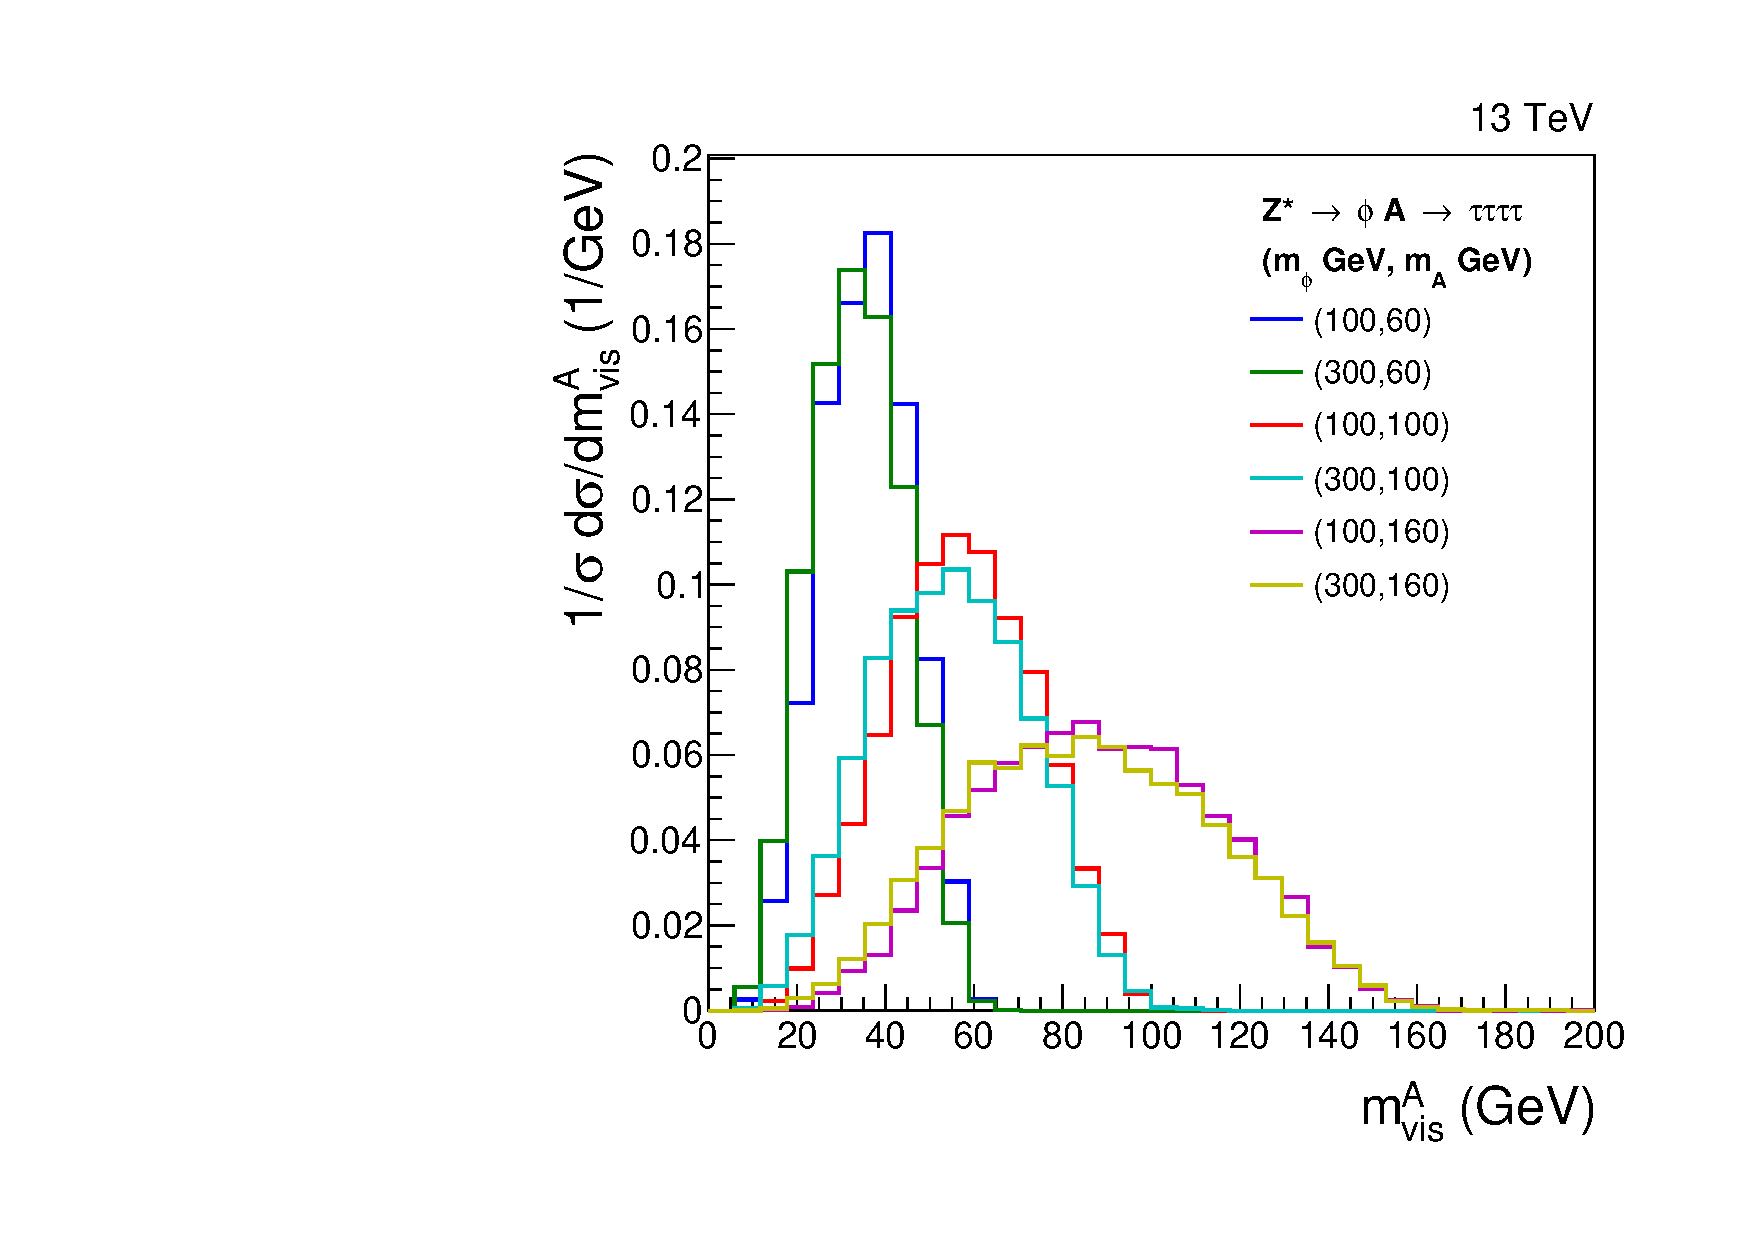
\includegraphics[width=0.49\textwidth]{Figures/mA_dist.pdf}}
    \subfloat[]{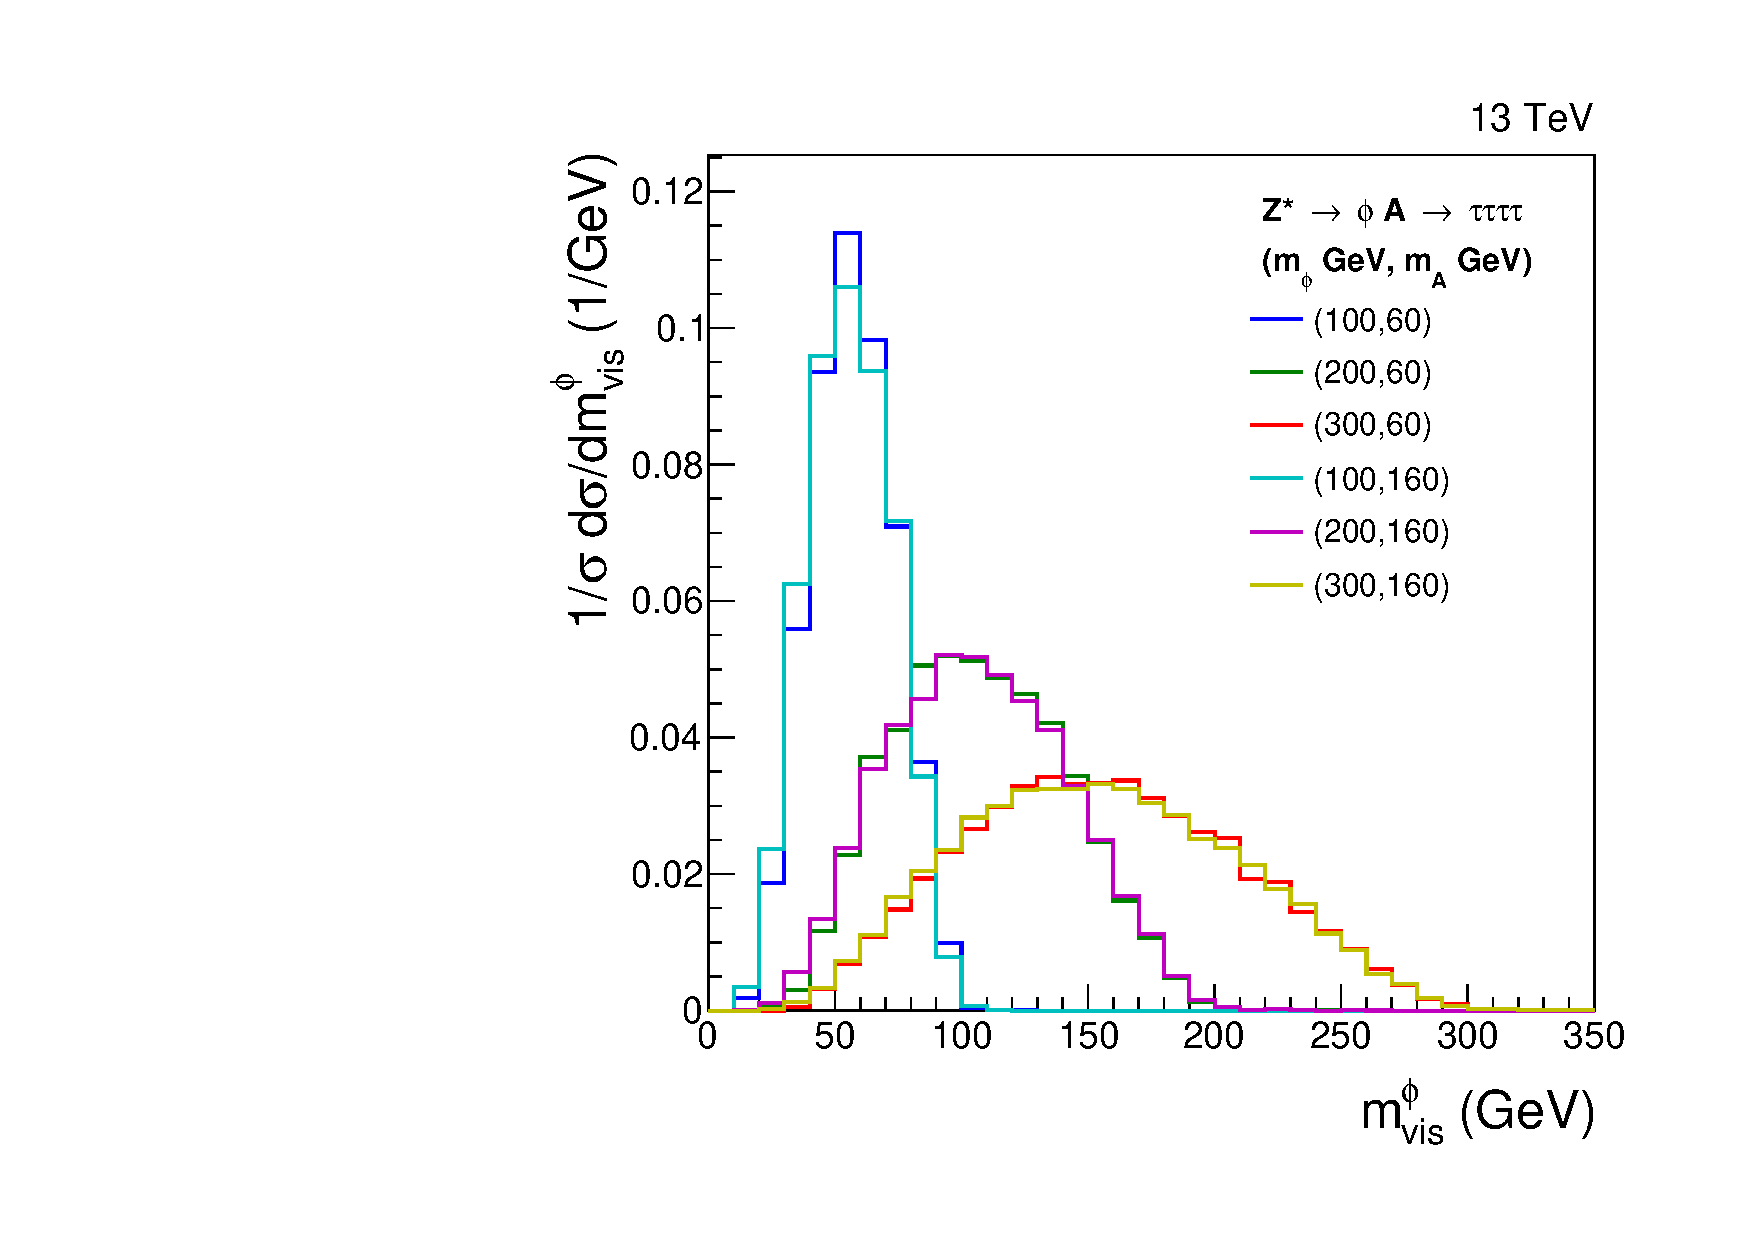
\includegraphics[width=0.49\textwidth]{Figures/mphi_dist.pdf}} 
\caption[Plots of the signal $m_{\tau\tau}$ generator level distributions of $\phi$ and A.]{Generator level distributions of the visible mass densities for A (a) and $\phi$ (b) for the signal process.}
\label{fig:4tau_gen_dist}
\end{figure}

The cross-sections in the alignment scenarios are also determined with this procedure and vary from 10 fb ($m_{A}=60$ GeV and $m_{\phi}=100$ GeV) to 650 fb ($m_{A}=160$ GeV and $m_{\phi}=300$ GeV), as shown in Figure~\ref{fig:4tau_xs}.
These are independent of $\tan\beta$, however, out of the alignment scenarios the cross-sections for H scales with $\sin^{2}(\beta-\alpha)$ and h scales with $\cos^{2}(\beta-\alpha)$. \\

\begin{figure}[!hbtp]
\centering
    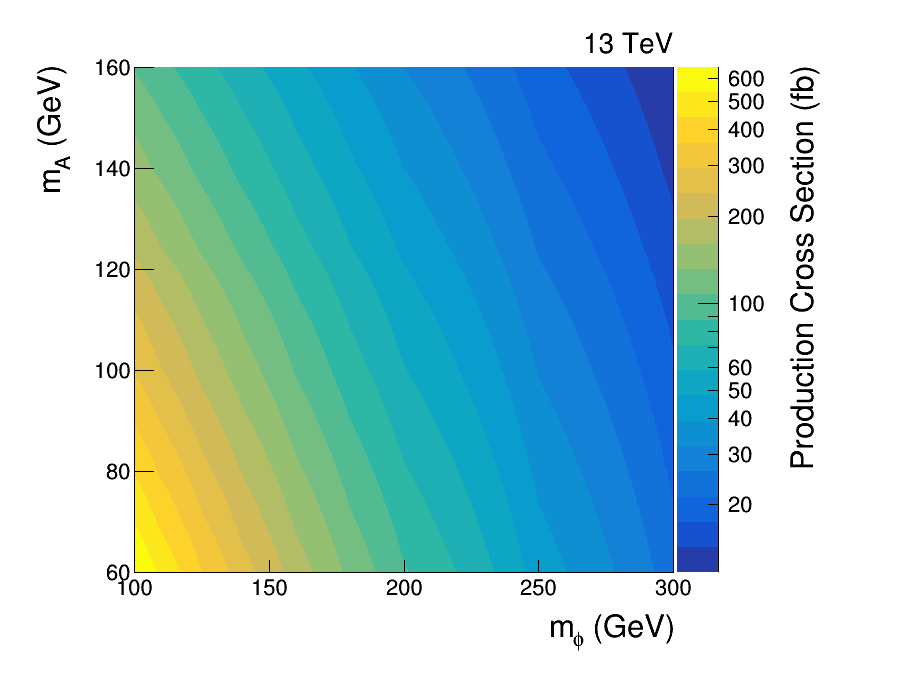
\includegraphics[width=0.8\textwidth]{Figures/cross_sections.png}
\caption[Plot of the production cross-sections for the $Z^{*} \rightarrow \phi A$ process.]{Calculated productions cross-sections for the $Z^{*} \rightarrow \phi A$ process, varying the masses of $\phi$ and A.}
\label{fig:4tau_xs}
\end{figure}

The branching fractions of $\phi$ and A to pairs of $\tau$ leptons are dependent on both $\tan\beta$ and $\beta-\alpha$.
For this analysis, the branching fractions are calculated using \textsc{2HDECAY} \cite{Krause:2018wmo}.
In the alignment scenarios, the $A\rightarrow\tau\tau$ branching fractions are approximately 1 above $\tan\beta \approx 2$, where below they sharply drop off and other processes such as $A\rightarrow b\bar{b}$ become dominant.
This is also true for $\phi\rightarrow\tau\tau$ branching fractions, except in the case where $m_\phi$ is greater than $m_A$ by more than $m_Z$, and so the $\phi\rightarrow ZA$ decay becomes kinematically feasible and can dominate at high $\tan\beta$.
Examples of this are shown in Figure~\ref{fig:4tau_br_1d}.
Out of the alignment scenario, the branching fractions of $\phi$ to $\tau$ leptons become smaller as the magnitude of the coupling of additional neutral Higgs bosons to $\tau$ leptons is reduced, whilst the $A$ branching fractions, like the couplings, are left unchanged.
An example of the $\phi$ branching fractions out of the alignment scenario is shown in Figure~\ref{fig:4tau_br_2d}.

\begin{figure}[!hbtp]
\centering
    \subfloat[]{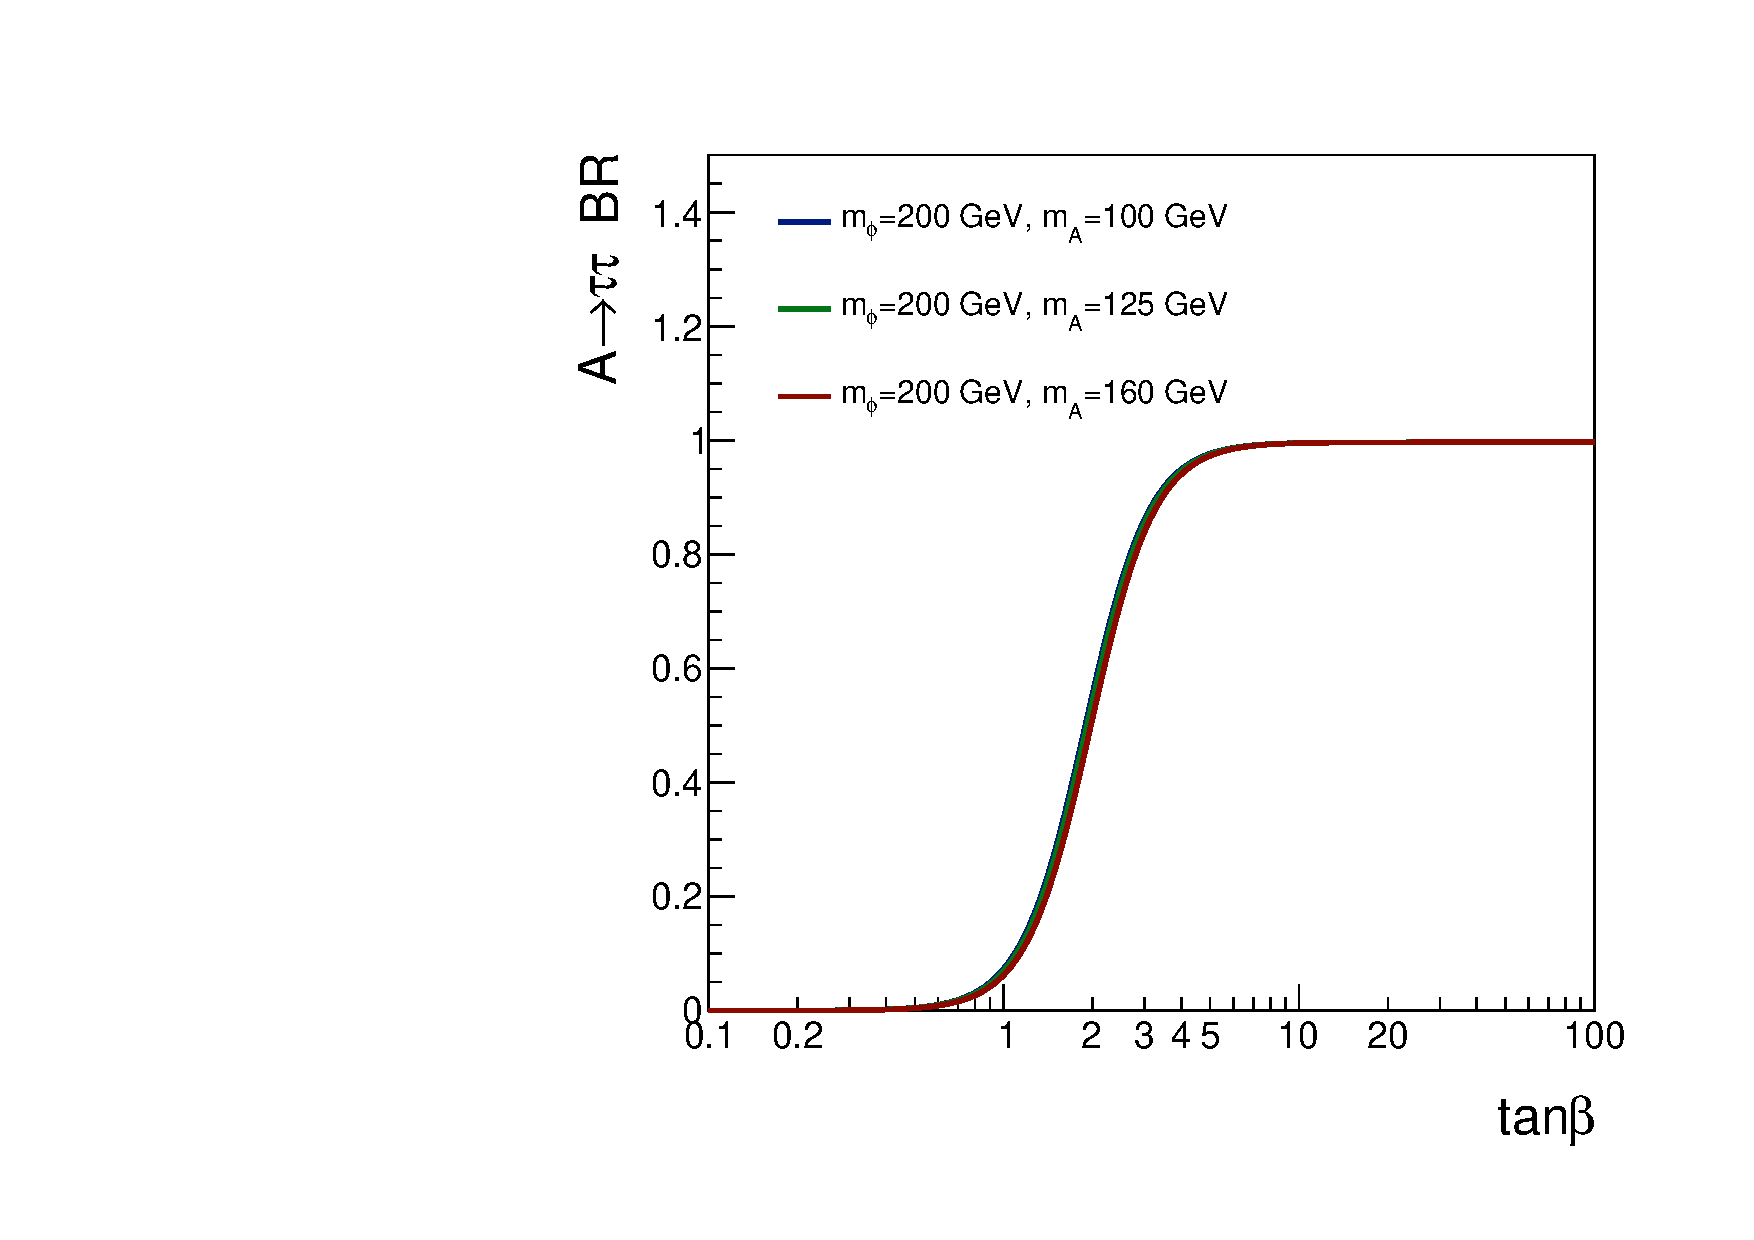
\includegraphics[width=0.49\textwidth]{Figures/A_br_plot_mphi200.pdf}}
    \subfloat[]{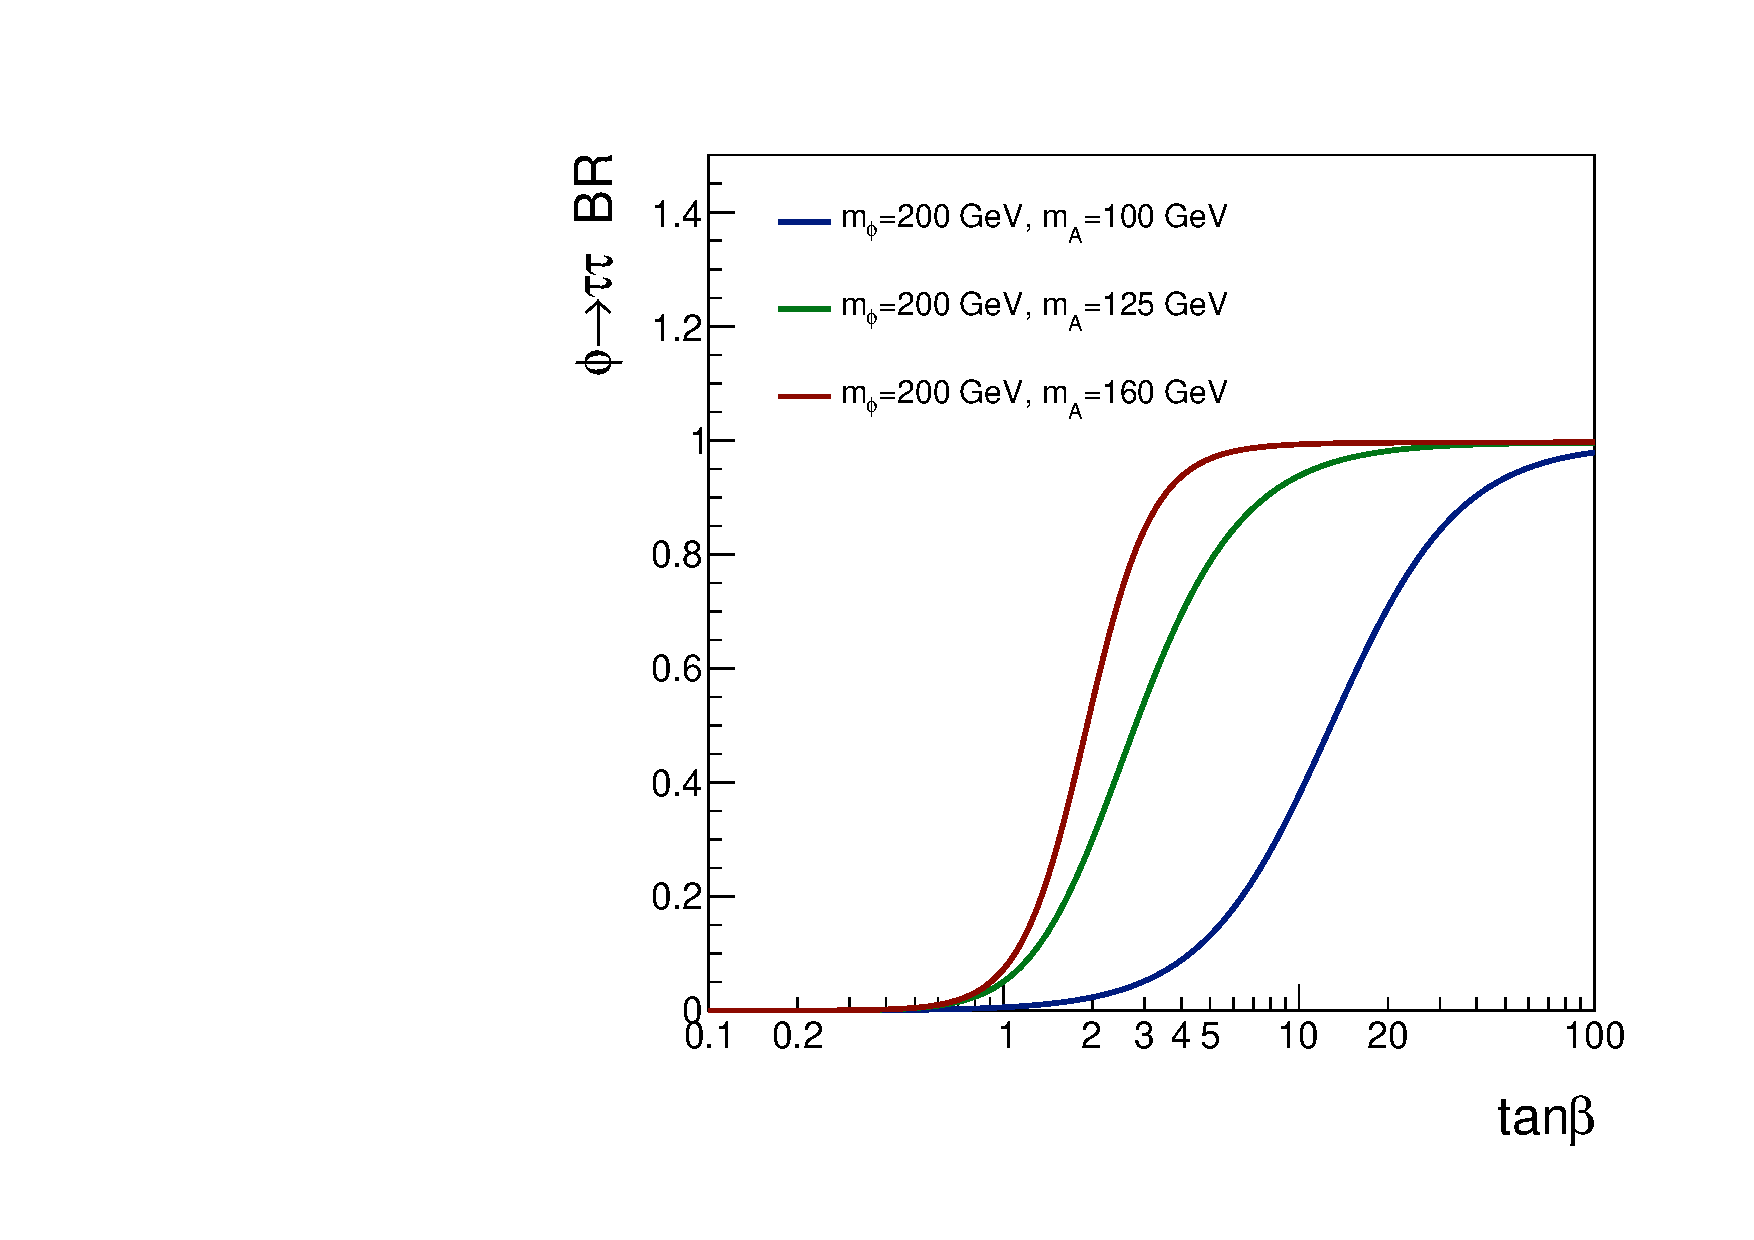
\includegraphics[width=0.49\textwidth]{Figures/phi_br_plot_mphi200.pdf}} 
\caption[Plots of the branching fractions $\phi$ and A to pairs of $\tau$ leptons in the alignment scenario.]{Calculated branching fractions of A (a) and $\phi$ (b) decaying to a pair of $\tau$ leptons for various mass scenarios.}
\label{fig:4tau_br_1d}
\end{figure}

\begin{figure}[!hbtp]
\centering
    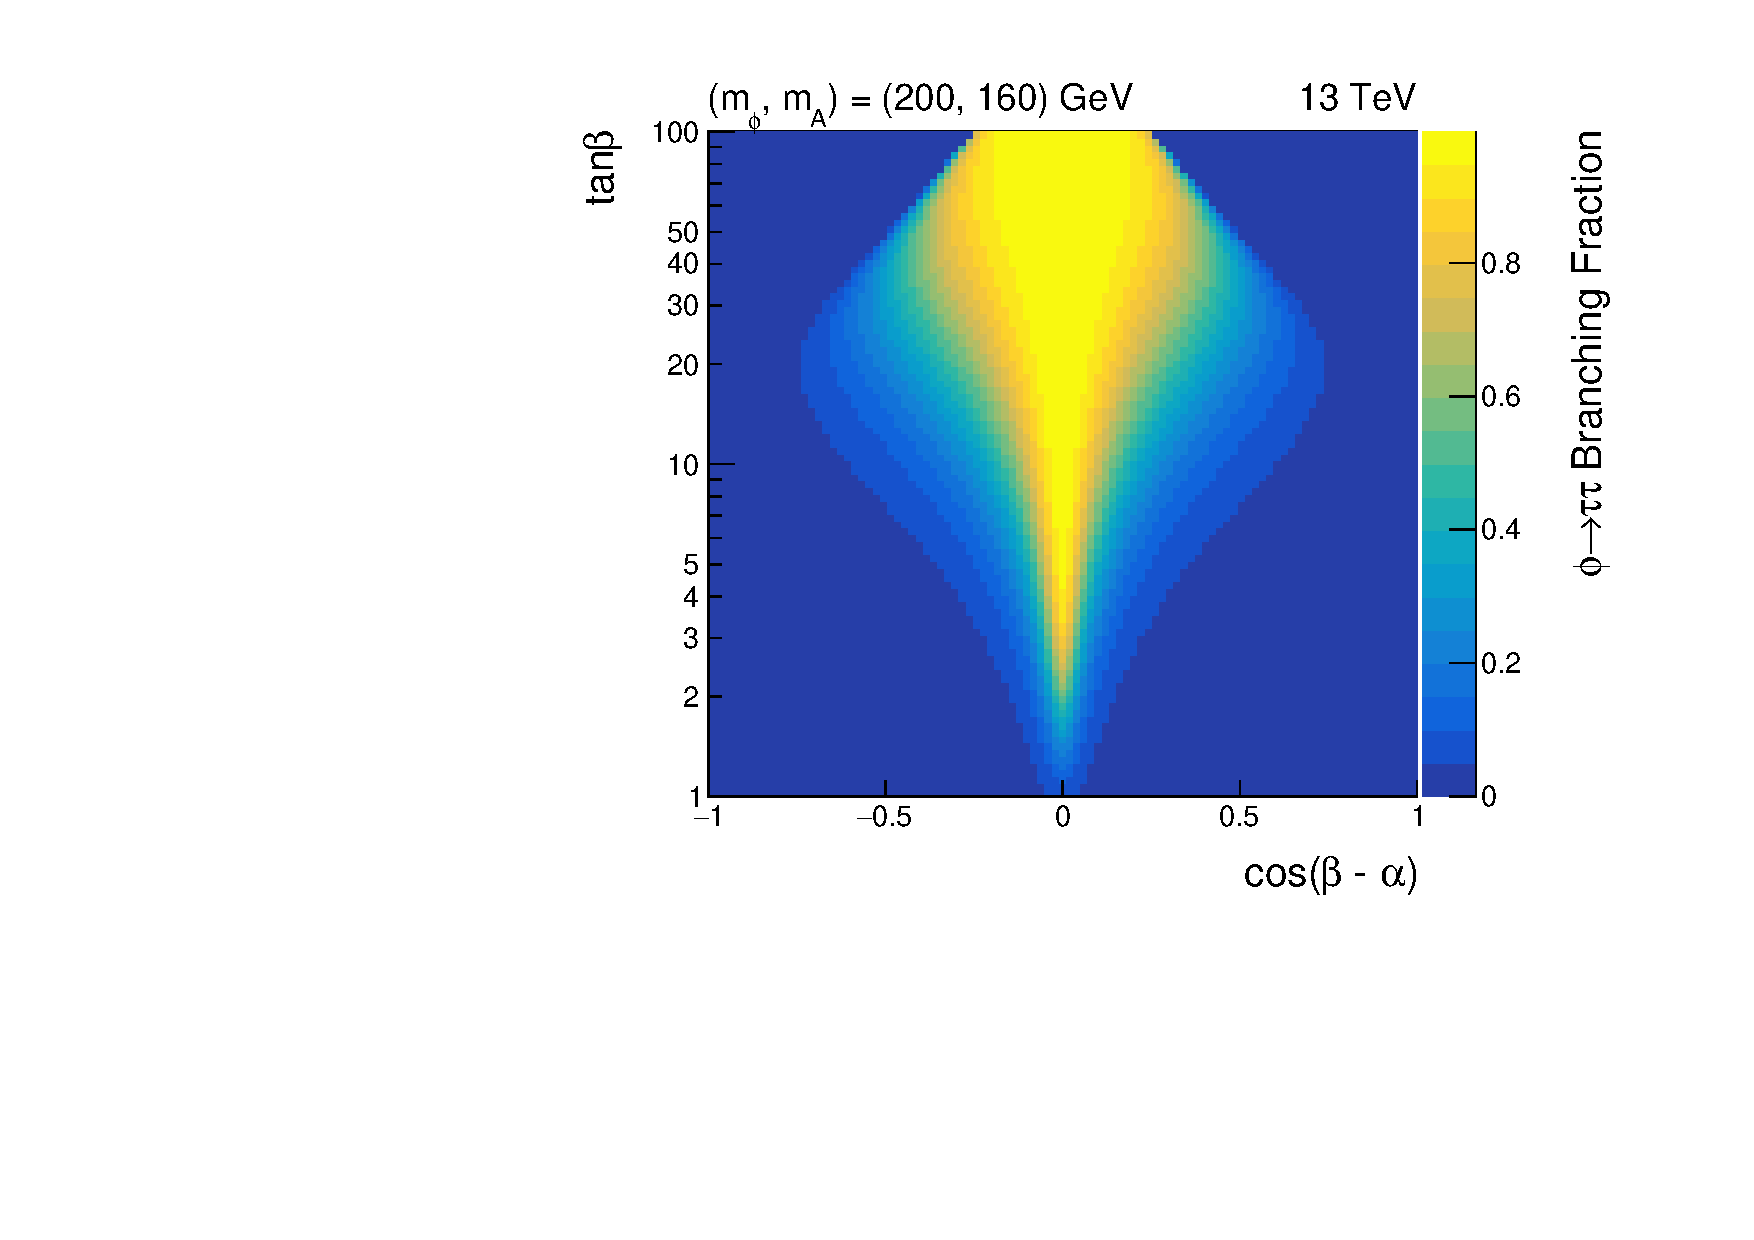
\includegraphics[width=0.7\textwidth]{Figures/phi_branching_fractions_mphi200_mA160.pdf}
\caption[Plot of the branching fractions of $\phi$ to pairs of $\tau$ leptons out of the alignment scenario.]{Calculated branching fractions in the $\cos(\beta-\alpha)$-$\tan\beta$ phase space for $\phi$ of mass 200 GeV decaying to a pair of $\tau$ leptons, in the scenario where $m_A = 160$ GeV.}
\label{fig:4tau_br_2d}
\end{figure}

\section{Event selection}

In comparison to Chapter~\ref{sec:bsm_H_to_tau_tau_analysis}, four $\tau$ leptons produce a much larger number of possible final states. 
All variations of $e$, $\mu$ and $\tau_h$ final state combinations and their branching fractions are shown in Table~\ref{tab:4tau_bf}.
Just under 90\% of the branching ratio goes to decay products containing two or more hadronic taus.
These are the main final states that are explored in this analysis. 
In addition to this, an orthogonal $\tau_h \tau_h \tau_h$ channel is added to target events where the reconstruction of the $\tau_h \tau_h \tau_h \tau_h$ channel loses a single $\tau_h$ object.
This can come about due to low triggering and identification efficiencies of $\tauh$ candidates, as well as the high $\pT$ thresholds required for both. \\
In total, the analysis consists of seven channels.

\begin{table}[!hbtp]
    \centering
    \begin{tabular}{|c|c|}
         \hline
         Channel & Branching Fraction  \\
         \hline
         \hline
         $e \tau_h \tau_h \tau_h$ & 19.4\% \\
         $\mu \tau_h \tau_h \tau_h$ & 18.9\% \\
         $\tau_h \tau_h \tau_h \tau_h$ & 17.6\% \\
         $e \mu \tau_h \tau_h$ & 15.6\% \\
         $e e \tau_h \tau_h$ & 8.0\% \\
         $\mu \mu \tau_h \tau_h$ & 7.6\% \\
         $e e \mu \tau_h$ & 4.3\% \\
         $e \mu \mu \tau_h$ & 4.2\% \\
         $e e e \tau_h$ & 1.5\% \\
         $\mu \mu \mu \tau_h$ & 1.4\% \\
         $e e e \mu$ & 1.4\% \\
         $e e \mu \mu$ & 0.6\% \\
         $e \mu \mu \mu$ & 0.4\% \\
         $e e e e$ & 0.1\% \\
         $\mu \mu \mu \mu$ & 0.1\% \\
         \hline
    \end{tabular}
    \caption[Branching fractions of four $\tau$ leptons.]{Branching fractions of four $\tau$ leptons, where e and $\mu$ represent the leptonic decay of the $\tau$ and $\tauh$ represent the hadronic decay of the $\tau$.}
    \label{tab:4tau_bf} 
\end{table}

\subsection{Trigger requirements}

Given that each final state is not exactly triggered on, there is no obvious choice for what triggers to use. 
A variety of triggers are available for individual and clusters of objects in the final state. 
The possible triggers for single objects are the single-e and single-$\mu$ triggers. 
This is not the case for the single-$\tau_h$ trigger as it has a $\pT$ threshold too high for it to be useful. 
The possible triggers for clusters of objects are the double-e, double-$\mu$, double-$\tau_h$, e-$\mu$ cross, $\mu$-$\tau_h$ cross and e-$\tau_h$ cross-triggers.
The cross-triggers and double-e/$\mu$ triggers are found to offer little improvement to the signal acceptance and so these events are not included.
Any combination of objects in the final state of a channel can be selected by these triggers and the union of events passing each iteration is taken. 
The trigger $\pT$ and $\eta$ thresholds for the remaining triggers (single-e/$\mu$ and double-$\tauh$) are equivalent to what is stated in Section~\ref{sec:trig_ditau}.

\subsection{Offline requirements}

All offline selections stated in this section are in addition to the object selection discussed in Section~\ref{sec:object_reconstruction}.
In this analysis, $\tau_h$ candidates are required to pass the \texttt{Loose} $D_{\text{jet}}^{\text{WP}}$.
The \texttt{VVLoose} $D_{e}^{\text{WP}}$ and \texttt{VLoose} $D_{\mu}^{\text{WP}}$ are used in all decay channels.
These working points are chosen to maximise the sensitivity of the analysis and looser cuts are used than in Chapter~\ref{sec:bsm_H_to_tau_tau_analysis} to ensure there are enough statistics to account for the stricter selection of more objects in the final states. \\

On top of the object selection, there are a few further selections on the total $\tau$ collection.
As the two $\tau$ pairs from the signal originate from two neutral additional Higgs bosons, the sum of charges of the fully reconstructed objects should be zero. 
This is applied in the decay channels where there are four objects. 
In the $\tau_h \tau_h \tau_h$ channel, as the assumption is that a $\tauh$ has been lost, the absolute value of the sum of the charges of the objects is required to be one.
To ensure the orthogonality between channels, a number of vetos are needed. 
Firstly, extra lepton vetos are used in all decay channels, where the absence of additional electrons and muons is required on top of those already part of the selected pair.
The kinematic, identification and isolation requirements on these extra leptons match the loosest cuts required for a nominally selected electron or muon.
Secondly, an extra $\tau_h$ veto is applied to the $\tau_h \tau_h \tau_h$ channel, to keep it orthogonal to the $\tau_h \tau_h \tau_h \tau_h$ channel.
To do this, any extra $\tau_h$ candidate passing the signal selection is vetoed.
The constraints set on the number of leptons and $\tau_h$ candidates for each channel are shown in Table~\ref{tab:leptonvetoes}. \\

\begin{table}[!hbtp]
   \centering
   \begin{tabular}{|l|c|c|c|}
   \hline
   \multicolumn{1}{|c|}{Channel} & e & $\mu$ & $\tau_h$ \\ \hline \hline
   $\tau_h \tau_h \tau_h \tau_h$ & 0 & 0     & $\geq$4        \\
   $\tau_h \tau_h \tau_h$        & 0 & 0     & 3        \\ 
   $\mu \tau_h \tau_h \tau_h$    & 0 & 1     & $\geq$3        \\
   $e \tau_h \tau_h \tau_h$      & 1 & 0     & $\geq$3        \\
   $e \mu \tau_h \tau_h$         & 1 & 1     & $\geq$2        \\
   $\mu \mu \tau_h \tau_h$       & 0 & 2     & $\geq$2        \\
   $e e \tau_h \tau_h$           & 2 & 0     & $\geq$2        \\ \hline
   \end{tabular}
   \caption[Number of objects required to be selected in each decay channel.]{Number of objects required to be selected in each decay channel.}
   \label{tab:leptonvetoes}
\end{table}

Finally, in channels containing an electron or a muon, a veto on events with one or more b-tagged jets is placed.
This is done to remove the $\ttbar$ background process in a region where little to no signal is expected.
This is not done in the fully $\tauh$ channels as the $\ttbar$ process is negligible. \\

\section{Search optimisation}

Due to the limited statistics in each decay channel, only minimal categorisation of events can be performed and the only divisions of the decay channels happen in final states with two light leptons and two $\tau_h$ candidates, where two categories are made.
These separate events where the light leptons have the same charge (\texttt{SS Leptons}) and where they have opposite charge (\texttt{OS Leptons}).
This is motivated to separate regions where specific background processes are dominant.
In particular, a large portion of the $ee\tauh\tauh$ and $\mu\mu\tauh\tauh$ channel backgrounds come from $Z\rightarrow \ell\ell$ (or $Z\rightarrow\tau\tau\rightarrow \ell\ell$) with two jets misidentified as $\tauh$ candidates, where the two light leptons are of opposite sign.
Similarly, the $e\mu\tauh\tauh$ channel contains more background events with an opposite sign electron and muon, from a Z decay via $\tau$ leptons or from the $\ttbar$ process.
There is less preference towards the light leptons being of opposite sign in the signal samples compared to in the background, and so more sensitivity to the signal is expected in the \texttt{SS Lepton} categories. 
A summary of the categorisation and b tag selection is shown in Figure~\ref{fig:4tau_categories}. \\

\begin{figure}[!hbtp]
\centering
    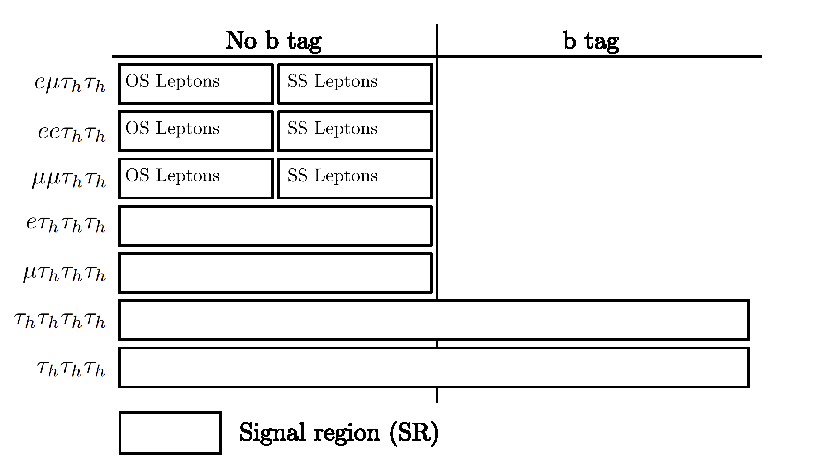
\includegraphics[width=0.85\textwidth]{Figures/event-categories_4tau.pdf}
\caption[Diagram of the categories used to extract $Z^{*}\rightarrow \phi A \rightarrow 4\tau$.]{Overview of the categories used for the extraction of the signal in the $Z^{*}\rightarrow \phi A \rightarrow 4\tau$.}
\label{fig:4tau_categories}
\end{figure}

Similarly to Section~\ref{sec:high_mass_optimisation}, events in each 10 analysis channels and categories are drawn out into a histogram based on the same discriminating variable, the total transverse mass ($m_{T}^{\text{tot
}}$).
However, as there are more objects in the final state, the definition is extended to what is shown below.
\begin{equation}
m_{T}^{\text{tot}} = \sqrt{ \sum_{i=1}^{N_\tau} m_{T}(\vec{p}_{T}^{\hspace{2pt}\tau_i},\vec{p}_{T}^{\hspace{2pt}\text{miss}})^2 + \sum_{i,j=1; i \neq j}^{N_\tau} m_{T}(\vec{p}_{T}^{\hspace{2pt}\tau_i},\vec{p}_{T}^{\hspace{2pt}\tau_j})^2 },  
\end{equation}
where $N_\tau$ is the number of objects in the final state, and $\tau_i$ refers to the visible products of the $i$th $\tau$ lepton.
This variable again provides excellent discriminating power between resonant signals compared to other non-peaking backgrounds, whilst still maintaining some separation between signal masses.
The sensitivity of this discriminating variable was tested against many others, including the visible masses of the two bosons which can be separated to $\approx 90\%$ efficiency, when the correct $\tau$ objects are selected. 
As $m_{T}^{\text{tot}}$ uses information about the whole event, in particular, the high $p_{T}$ objects and high \ac{MET} from many $\tau$ decays, a greater sensitivity to the signal is observed. \\

In this analysis, many of the histograms contain very few background events and to minimise statistical fluctuations in the background templates, histogram bins are merged based on the fractional statistical uncertainty of each bin.
This leads to many single and minimally binned channels/categories where background statistics are low but signal sensitivity is high and a few finely binned and high statistic channels/categories able to better classify the signal, if one is observed.
 
\section{Background modelling overview}

The backgrounds are split into three categories:
\begin{enumerate}[i)]
  \item Events containing only genuine $\tau$ leptons.
  \item Events with one or more jets misidentified as a $\tauh$ candidate (\jtth).
  \item Events with one or more light leptons misidentified as a $\tauh$ candidate and no \jtth objects. 
\end{enumerate}

Background contributions from (i) are mostly from gluon and quark-initiated di-Z production and are modelled using \ac{MC}.
The details and validation of this modelling are described in Section~\ref{sec:zz_modelling}.
Background (ii) accounts for a number of different processes with \jtth candidates.
Examples of this are single-Z, single-W and $\ttbar$ productions with additional jets in the events being misidentified.
This is modelled with a fake factor method, similar to what is described in Section~\ref{sec:ff}, but using \ac{ML} to improve upon the method, and discussed further in Section~\ref{sec:ml_ff}.
Contribution (iii) is small in comparison to the others and modelled with \ac{MC}.
Events with jets misidentified as light leptons and no jets misidentified as $\tauh$ candidates have been checked with \ac{MC} and deemed negligible in all channels. \\

All \ac{MC} background samples described in Section~\ref{sec:background_modelling} are modelled in the same manner.  
In addition, tri-boson samples are used that are generated using \MGvATNLO at \ac{NLO} precision~\cite{Alwall:2011uj}.
All corrections described in Section~\ref{sec:ditau_corrections} are applied to \ac{MC}, with extra corrections applied to the ZZ process, which is detailed in Section~\ref{sec:zz_modelling}.

\section{ZZ modelling}
\label{sec:zz_modelling}

The di-Z background shapes, where there are no \jtth candidates are modelled using \ac{MC}.
The cross-sections for this analysis are scaled to higher-order precisions than generated using K factors.
For quark-initiated di-Z production, \POWHEG~2.0~\cite{Nason:2004rx,Frixione:2007vw,Alioli:2010xd,Jezo:2015aia} is used to determine \ac{NNLO}/\ac{NLO} \ac{QCD} and electroweak corrections as a function of $m_{ZZ}$, which takes an average value of $\approx 1.2$.
Gluon initiated di-Z production corrections from \ac{LO} to \ac{NNLO} are derived with HNNLO v2~\cite{PhysRevLett.98.222002}, again as a function of $m_{ZZ}$.
This gives a much larger correction, equal to $\approx 2$.
The modelling is validated using a $\mu\mu\mu\mu$ final state and good agreement is observed between data and simulation.
Identical object selection is applied as stated in Section~\ref{sec:object_reconstruction}, except to ensure better statistics within the channel, the muon $\Irel$ cut is loosened to 0.35.
The charges of the muon candidates are similarly required to sum to one and no vetos on the number of b jets in the event is applied.
Plots of this are shown in Figure~\ref{fig:4tau_mmmm}. \\

\begin{figure}[!hbtp]
\centering
    \subfloat[]{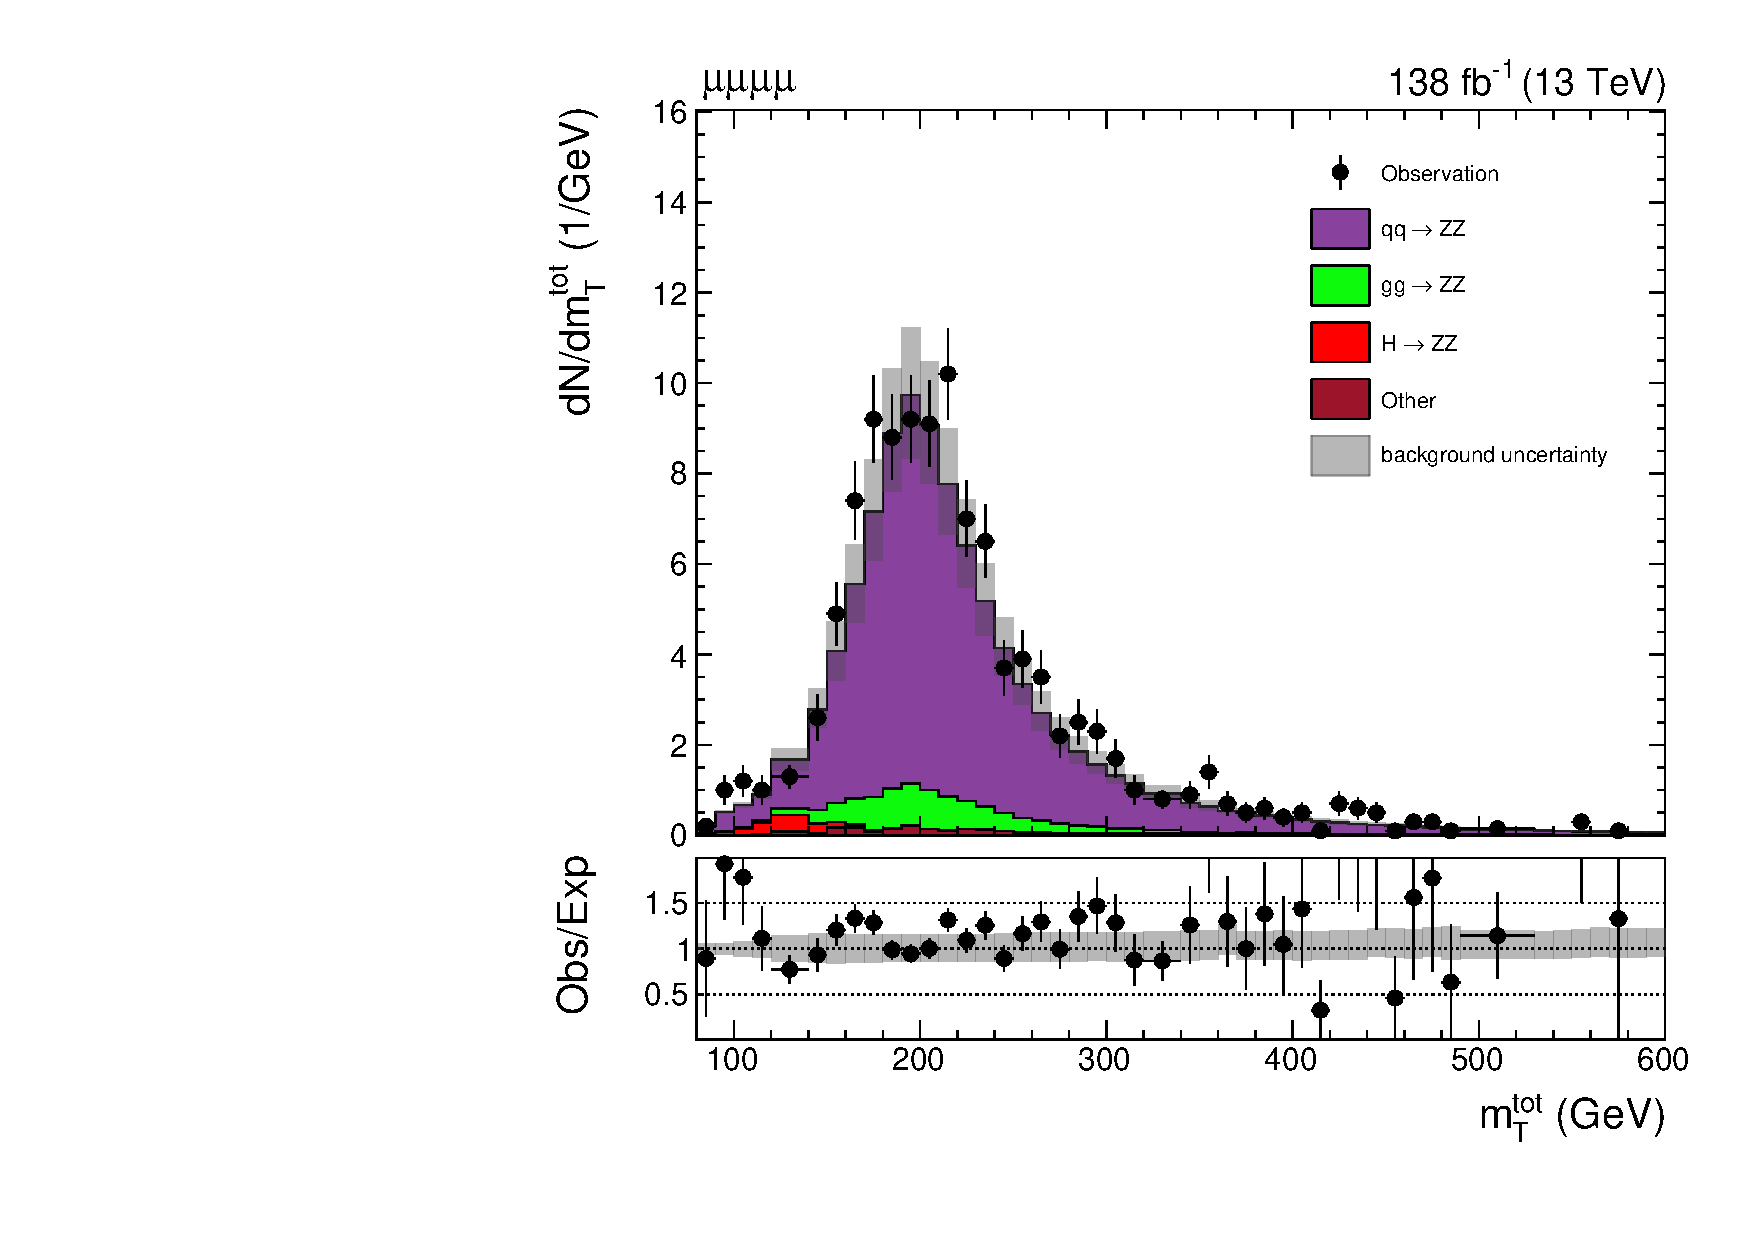
\includegraphics[width=0.49\textwidth]{Figures/mt_tot_signal_mmmm_inclusive_all.pdf}}
    \subfloat[]{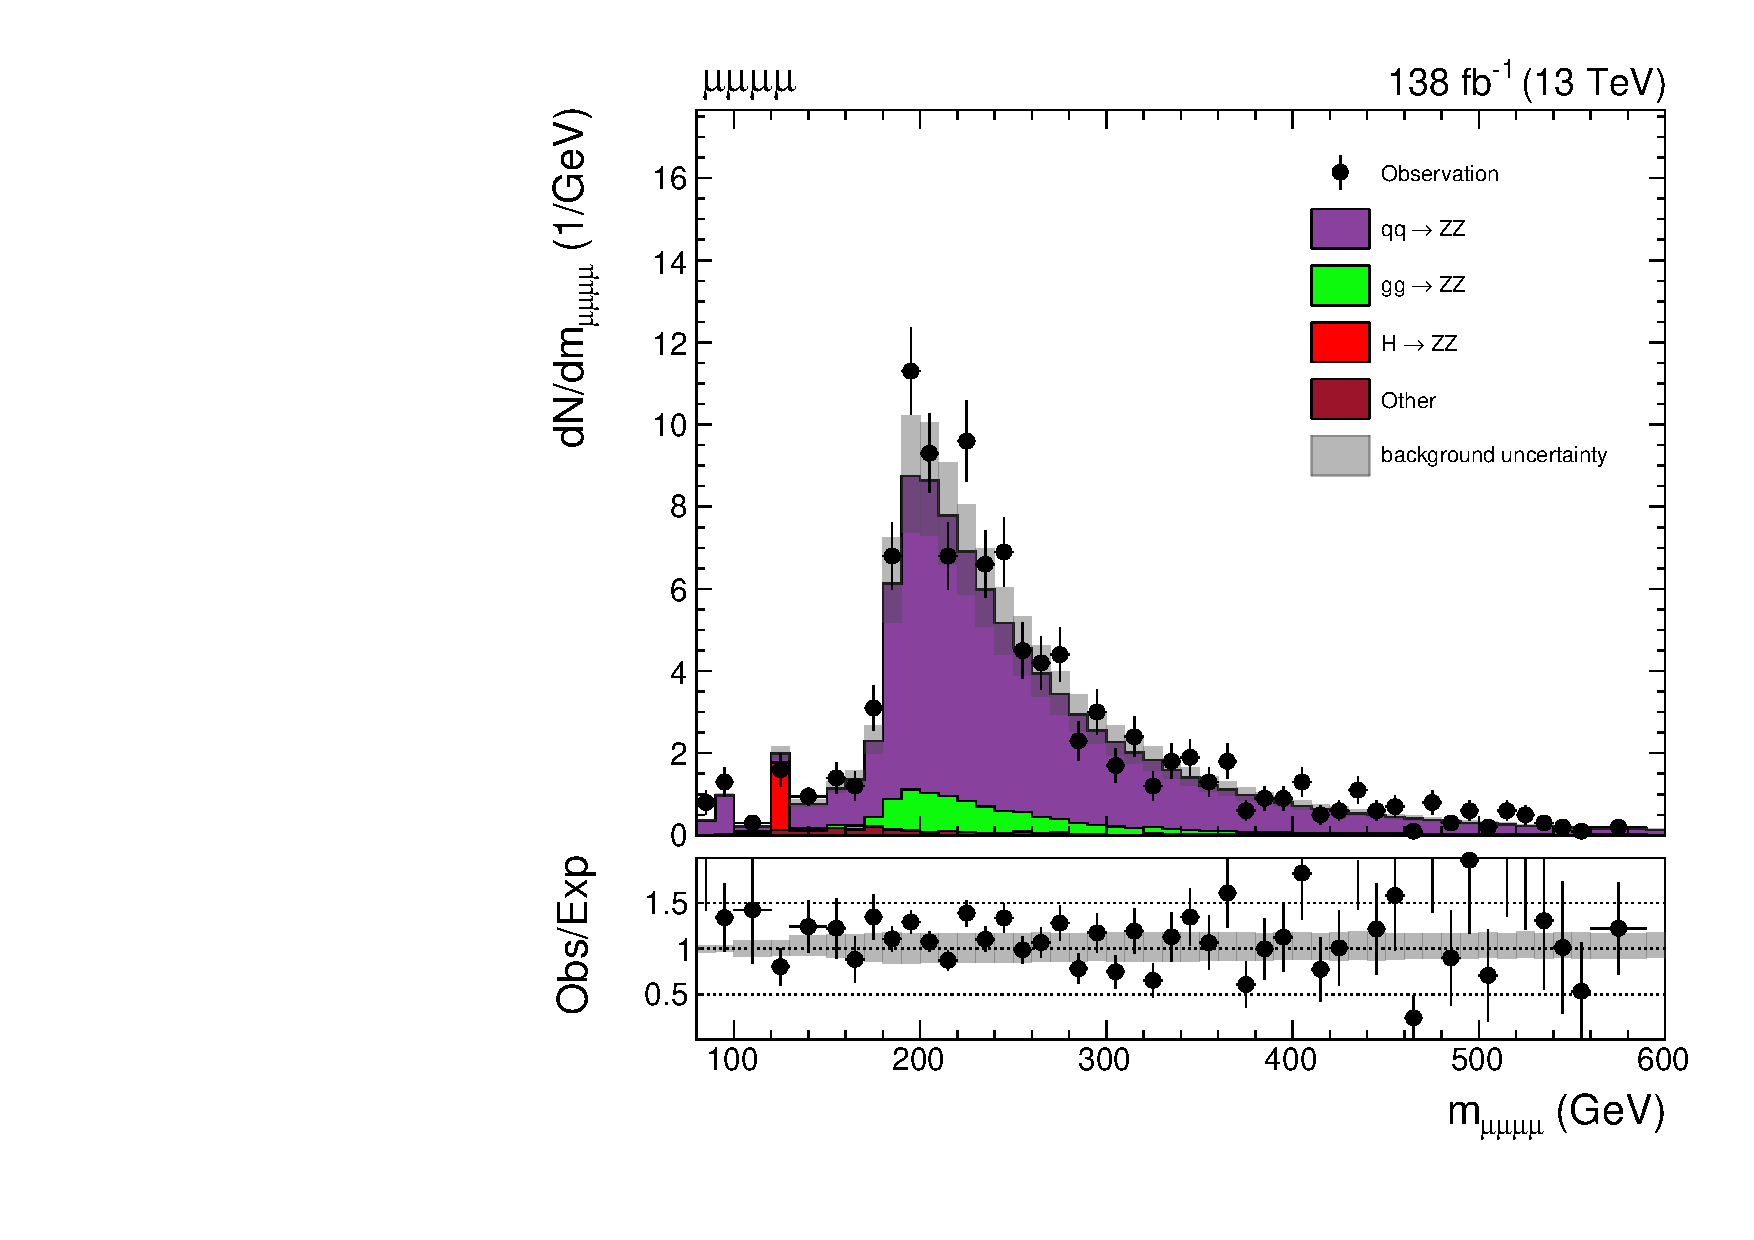
\includegraphics[width=0.49\textwidth]{Figures/mvis_1234_signal_mmmm_inclusive_all.pdf}} 
\caption[Plots of the distributions in the $\mu\mu\mu\mu$ channel.]{Distributions in the $\mu\mu\mu\mu$ channel are shown for the total transverse mass $m_{T}^{\text{tot}}$ (a), and the total mass $m_{\mu\mu\mu\mu}$ (b) variables. The solid histograms show the stacked background predictions.}
\label{fig:4tau_mmmm}
\end{figure}


\section{Machine learning fake factor method}
\label{sec:ml_ff}

The $\FF$ method, as described in Section~\ref{sec:ff}, is an algorithm used to model the \jtth backgrounds.
It uses classical reweighting techniques, such as binning the two regions and applying a fit to the ratio in a chosen parametrisation.
This method faces difficulties when approached with high dimensional dependence on parametrisation.
In this scenario, classical \say{bin and fit} methods can break down, as for every new parameter included the statistics of each fit are reduced.
A compromise must then be reached between variable dependence and fit statistics and this is the case for the $\pT^{\text{jet}}/\pT^{\tauh}$ binning described in Section~\ref{sec:ff_params}.
It is also the case, that the analysis in Chapter~\ref{sec:bsm_H_to_tau_tau_analysis} uses well-checked assumptions on, for example, the consistency of $\tauh$ decay modes from determination to signal regions, to average across the dependencies on this variable when calculating $\FF$, however, this will not always be the case.
Also binned upon in the previous search, is the process dependence of the $\FF$.
The binning used is an admission that the relevant parametrisation of the $\FF$ between processes is too complicated to model with \say{bin and fit} methods.
It can also be seen that the initial fits, do not do a good job of modelling all variables as corrections are needed. \\

There is a final problem with using a $\FF$ method as described when there are multiple $\tauh$ candidates in final states. 
In the $\tauh\tauh$ channel of the previous analysis, the $\FF$ were only calculated from the leading $\tauh$ candidate.
This was valid, as the dominant backgrounds had two \jtth candidates rather than one genuine $\tauh$ and one \jtth candidate.
However, for this search, this assumption is not valid. \\

All of these reasons motivate a more generalised and smarter method to model \jtth backgrounds, as well as the extra importance of modelling these backgrounds where there are more $\tauh$ candidates in the final state.
This is done by utilising \ac{ML} and in particular using a \ac{BDT} for the purpose of multi-dimensional reweighting. \\ 

\subsection{BDT reweighter}

Reference~\cite{Rogozhnikov:2016bdp} proposes a new method for reweighting utilising \ac{ML} techniques to solve the issues with dimensionality. 
It looks to optimise the regions that most need reweighting. 
One good way to do this is using a decision tree, as with this the data can be split into \say{leafs} by checking simple conditions.
To best choose the regions that need reweighting the algorithm looks to maximise the symmetrised $\chi^2$,

\begin{equation}
\chi^2 = \sum_{\text{leaf}} \frac{(w_{\text{leaf, 1}}-w_{\text{leaf, 2}})^2}{(w_{\text{leaf, 1}}+w_{\text{leaf, 2}})^2},
\end{equation}

where $w_{\text{leaf, 1}}$ and $w_{\text{leaf, 2}}$ are the entries weights in each leaf of the decision tree from the two datasets.
The larger the value of $\chi^2$, the more important reweighting is in this region. 
This tree is utilised many times in the reweighting algorithm, shown below:

\begin{enumerate}[i)]
\item Input training datasets 1 and 2 with a large number of variables.
\item Build a tree as stated above. If not the first loop, use newly determined weights for dataset 2.
\item Compute predictions in the leafs $r_{\text{leaf}} = \log\frac{w_{\text{leaf, 1}}}{w_{\text{leaf, 2}}}$. The logarithm is taken so weights in different trees can be summed as usually done in boosting.
\item In each leaf, dataset 2 events are weighted by $w = w \times e^{r_{\text{leaf}}}$.
\end{enumerate}

The final two steps are identical to the first approach except for the use of the logarithm for convenience using boosting. 
The major difference is how the bins used for reweighting are found, and this step is repeated multiple times. \\

\subsection{Fitting regions}

Unlike the standard $\FF$ method, statistics are not a problem using the \ac{BDT} reweighter when choosing which variables you can use to parametrise the $\FF$. 
Therefore, rather than fitting two fake factor regions separately and then a correction from the sideband to signal region to account for missing parametrisation, regions A, B and D from Figure~\ref{fig:ff_schematic} are fit simultaneously to improve statistics. 
Also, all $\tauh$ candidates are fit simultaneously as separate entries in the dataset and for each $\tauh$ in the event, the remaining $\tauh$ candidates are named the alternative $\tauh$ candidates. 
The sideband variable definitions and cuts, with respect to Figure~\ref{fig:ff_schematic}, are shown below. \\

\begin{enumerate}[i)]
   \item $ee\tauh\tauh$, $e\mu\tauh\tauh$, $\mu\mu\tauh\tauh$, $e\tauh\tauh\tauh$ and $\mu\tauh\tauh\tauh$  \\
     \indent $y_C$: The sum of $\tauh$ candidates is required to be 0. \\
     \indent $y_A$: The sum of $\tauh$ candidates is required to not be 0. \\
     \indent $x_C$: All alternative $\tau_h$ candidates pass the \texttt{Loose} $D_{\text{jet}}^{\text{WP}}$. \\
     \indent $x_D$: At least one alternative $\tau_h$ candidate fails the \texttt{Loose} $D_{\text{jet}}^{\text{WP}}$ but has $D_{\text{jet}}^{\text{score}} > 0.1$.
  \item $\tauh\tauh\tauh$ \\
     \indent $y_C$: The absolute value of the sum of $\tauh$ candidates is required to be 1. \\
     \indent $y_A$: The absolute value of the sum of $\tauh$ candidates is required to not be 1. \\
     \indent $x_C$: All alternative $\tau_h$ candidates pass the \texttt{Loose} $D_{\text{jet}}^{\text{WP}}$. \\
     \indent $x_D$: At least one alternative $\tau_h$ candidate fails the \texttt{Loose} $D_{\text{jet}}^{\text{WP}}$ but has $D_{\text{jet}}^{\text{score}} > 0.1$.
\end{enumerate}

These selections mimic what is done for the $\tauhtauh$ channel $\FF$ from Section~\ref{sec:ff_dr}, where the definitions of the alternative sideband variable are extended to more than one other $\tauh$ candidate.
The $D_{\text{jet}}^{\text{score}} > 0.1$ selection is used as the alternative $\tauh$ identification selection for this analysis and is also then extended to the alternative $\tauh$ candidates for this selection.
A cut on the score is used instead of a working point as the loosest defined working point does not provide enough statistics to ensure a good fit. \\

Extrapolating the regions used for fitting to the $\tau_h \tau_h \tau_h \tau_h$ channel, there would be some overlap in the fitting region with the $\tau_h \tau_h \tau_h$ signal region. 
As this region is expected to be sensitive to signal, this is not used to model jet $\rightarrow\tauh$ backgrounds in the $\tau_h \tau_h \tau_h \tau_h$ channel. 
Instead, the fit from the $\tau_h \tau_h \tau_h$ channel is used. 
There are a few variables that are defined differently in the fit between the two channels due to the difference between the four to three objects selected. 
Therefore, when getting $\FF$ in the $\tau_h \tau_h \tau_h \tau_h$, the lowest $D_{\text{jet}}^{\text{score}}$ unused $\tauh$ candidate is dropped and the variables are recalculated. 
This candidate is chosen to be removed to best mimic the initial selection of the $\tauh$ candidates, where they are sorted by $D_{\text{jet}}^{\text{score}}$ and the highest-scoring candidates are chosen. 
As shown later in this section, there is no major dependence on the shifted variables and any effects from this removal are covered within the uncertainty model. \\

\subsection{Variables used}

The variables used have been shown to have $\FF$ dependence previously~\cite{CMS:2020rpr,CMS:2022rbd}, and additional properties of the $\tauh$ candidate and the event. 
Also added are the variables that take you from A to C and D to C, from Figure~\ref{fig:ff_schematic}. 
As all years are fit together, to account for any differences in $\FF$ from year to year, this is also added. 
The final variable added is the $\pT$-ordered ranking of the $\tauh$ candidates in the event.
All the variables used are shown below.

\begin{enumerate}[i)]
\item The \ac{HPS} decay mode of the $\tauh$ candidate.
\item $\pT$ of the $\tauh$ candidate.
\item The ratio of the $\pT$ of the jet that seeds the \ac{HPS} reconstruction to the $\pT$ of the $\tauh$ candidate.
\item $\eta$ of the $\tauh$ candidate.
\item The charge of the $\tauh$ candidate.
\item A boolean of whether the $\tauh$ candidate passes a leg of the double-$\tauh$ trigger.
\item The total charge of the combined objects.
\item The boolean of whether $D_{\text{jet}}^{\text{WP}}$ passes to $\texttt{Loose}$ WP for the alternative $\tauh$ candidates. These are sorted by $\pT$.
\item Era of data taking.
\item $\tauh$ $\pT$ ordered event rank.
\end{enumerate}

\subsection{Machine learning subtraction method}

In the standard $\FF$ method, histograms are used to fit the $\FF$ rather than datasets. 
Using histograms, the small fraction of events which are not \jtth objects can easily be subtracted off. 
To do this, the data histogram is subtracted from by a stacked \ac{MC} background produced with generator matching ensuring the event is not a \jtth object and this produces a data-\ac{MC} hybrid histogram of predicted \jtth events.
However, subtraction is not possible with a full dataset and negative weights do not work with the \ac{BDT} reweighter. 
Therefore, the only option is to remove like-for-like events in data compared to the non \jtth generator matched \ac{MC}.
An example of this is template matching, which takes an event and can find the closest event in another dataset.
But as the fitting dataset is highly dimensional, this requires too much computation.
The solution proposed for this is to use a \ac{BDT} to reduce the dimensionality of the datasets, to effectively the one dimension of an output score of a simple binary classifier. \\

\begin{enumerate}[i)]
  \item In each channel, all \ac{MC} in the fitting region is stacked and scaled to cross-section (via weighting) and the variables used for reweighting are put into a dataset.
  \item \jtth and non \jtth objects are separated into the two classes that will be used for binary classification.
  \item To ensure unbiased training, the weights of the two categories are normalised to one another.
  \item A \ac{BDT} is then trained to separate whether the \ac{MC} is a \jtth object or not.
  \item The scores of the \ac{BDT} for how likely the entry is not a \jtth object is added to the dataset.
  \item The scores of the non \jtth candidates are drawn into a histogram with a number of bins suitable for the number of statistics and rescaled to the cross-section to best match what would be observed in data.
  \item The output score of the \ac{BDT} is added to data events
  \item Each bin of the \ac{MC} histogram is then looped through:
  \begin{itemize}
    \item Data entries with \ac{BDT} score within the range of the bin are selected.
    \item Entries within this bin are then randomly sampled and removed.
    \item This stops when the number of events removed equals the number of non \jtth objects predicted in the \ac{MC} histogram bin.
  \end{itemize}
\end{enumerate} 

This method then gives a data-\ac{MC} hybrid method to determine a dataset of predicted \jtth candidates and should give near identical results when drawing out histograms in all variables compared to subtracting off \ac{MC} non \jtth candidates from a data histogram as used in the original $\FF$ method.
It allows for non \jtth like candidates to be sampled and removed to the correct yield through all variables.
It is important to remove events throughout the \ac{MC} non jet $\rightarrow\tauh$ \ac{BDT} score histogram as if only the highest score events were removed, these events would come primarily from the tails of the distribution where it is easiest to separate. \\

An uncertainty is placed on the performance of this algorithm with respect to histogram subtraction.
This is calculated by drawing each variable used for the method into a histogram with binning chosen to ensure a sensible number of events in each bin.
An uncertainty is then derived from the difference in prediction between the histogram and \ac{BDT} subtraction. \\

To validate this method, example histograms with this uncertainty are shown for the $\mu\tauh\tauh\tauh$ pass $\tauh$ identification region in Figure~\ref{fig:4tau_ff_subtraction}, comparing the \ac{BDT} subtraction method and histogram subtraction method for a few of the fitted variables. \\

\begin{figure}[!hbtp]
\centering
    \subfloat[]{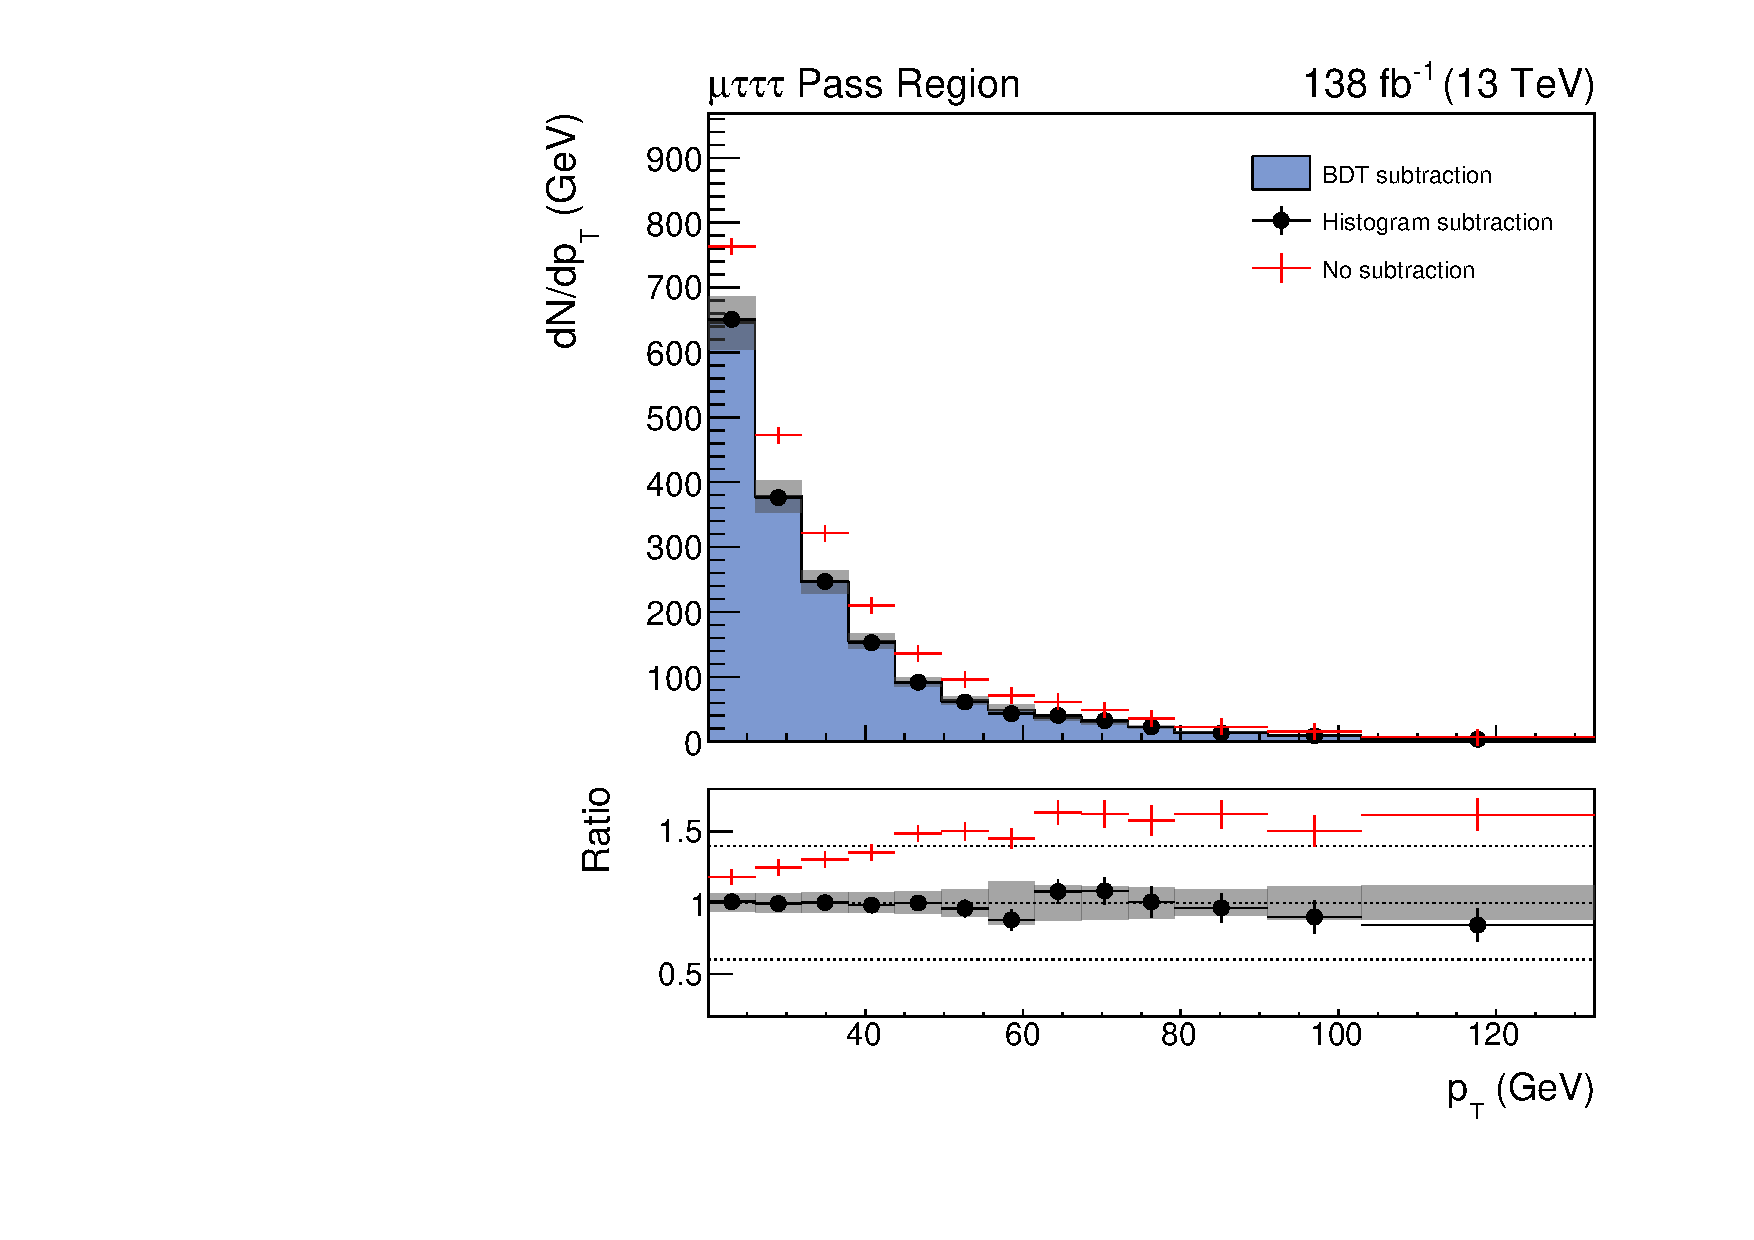
\includegraphics[width=0.45\textwidth]{Figures/subtraction_plot_pt_1_mttt_pass.pdf}}
    \subfloat[]{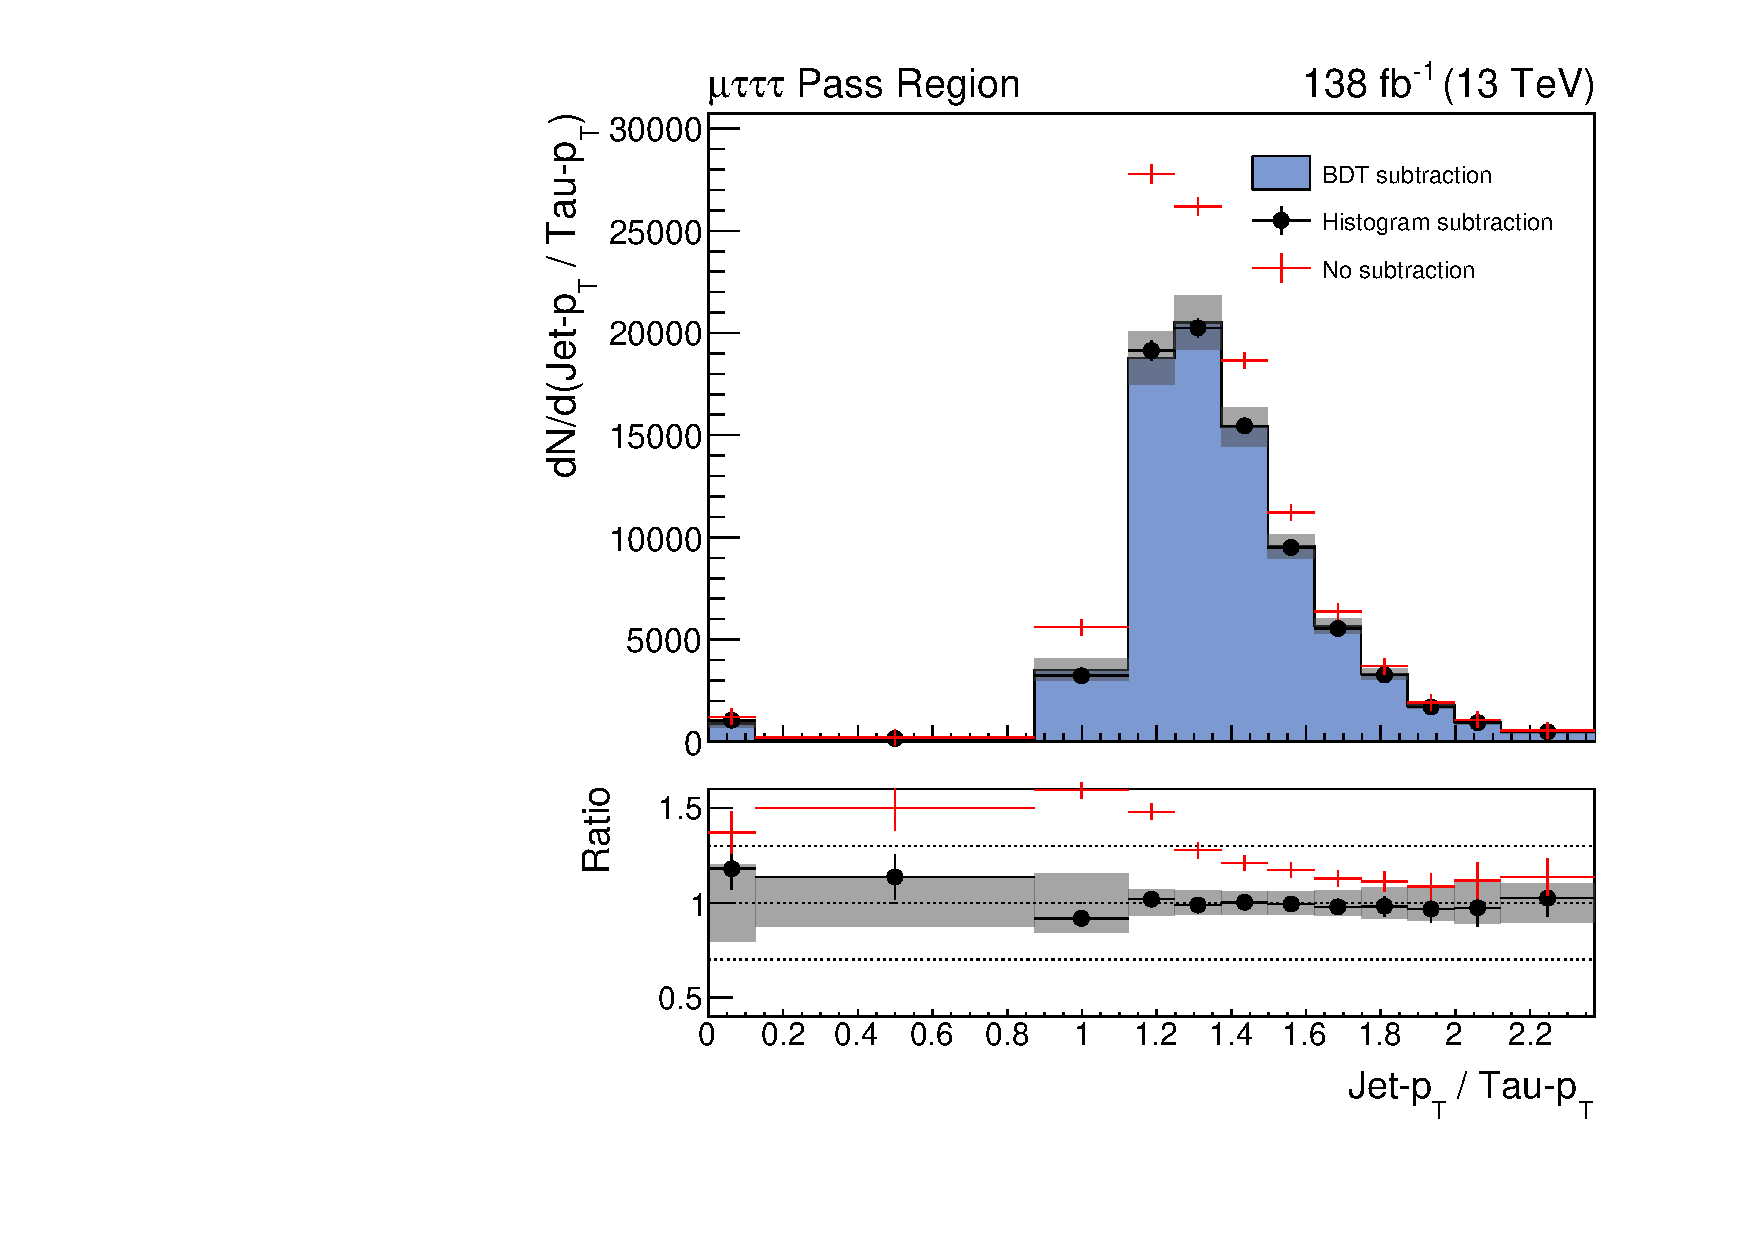
\includegraphics[width=0.45\textwidth]{Figures/subtraction_plot_jet_pt_1_divide_pt_1_mttt_pass.pdf}} \\
    \subfloat[]{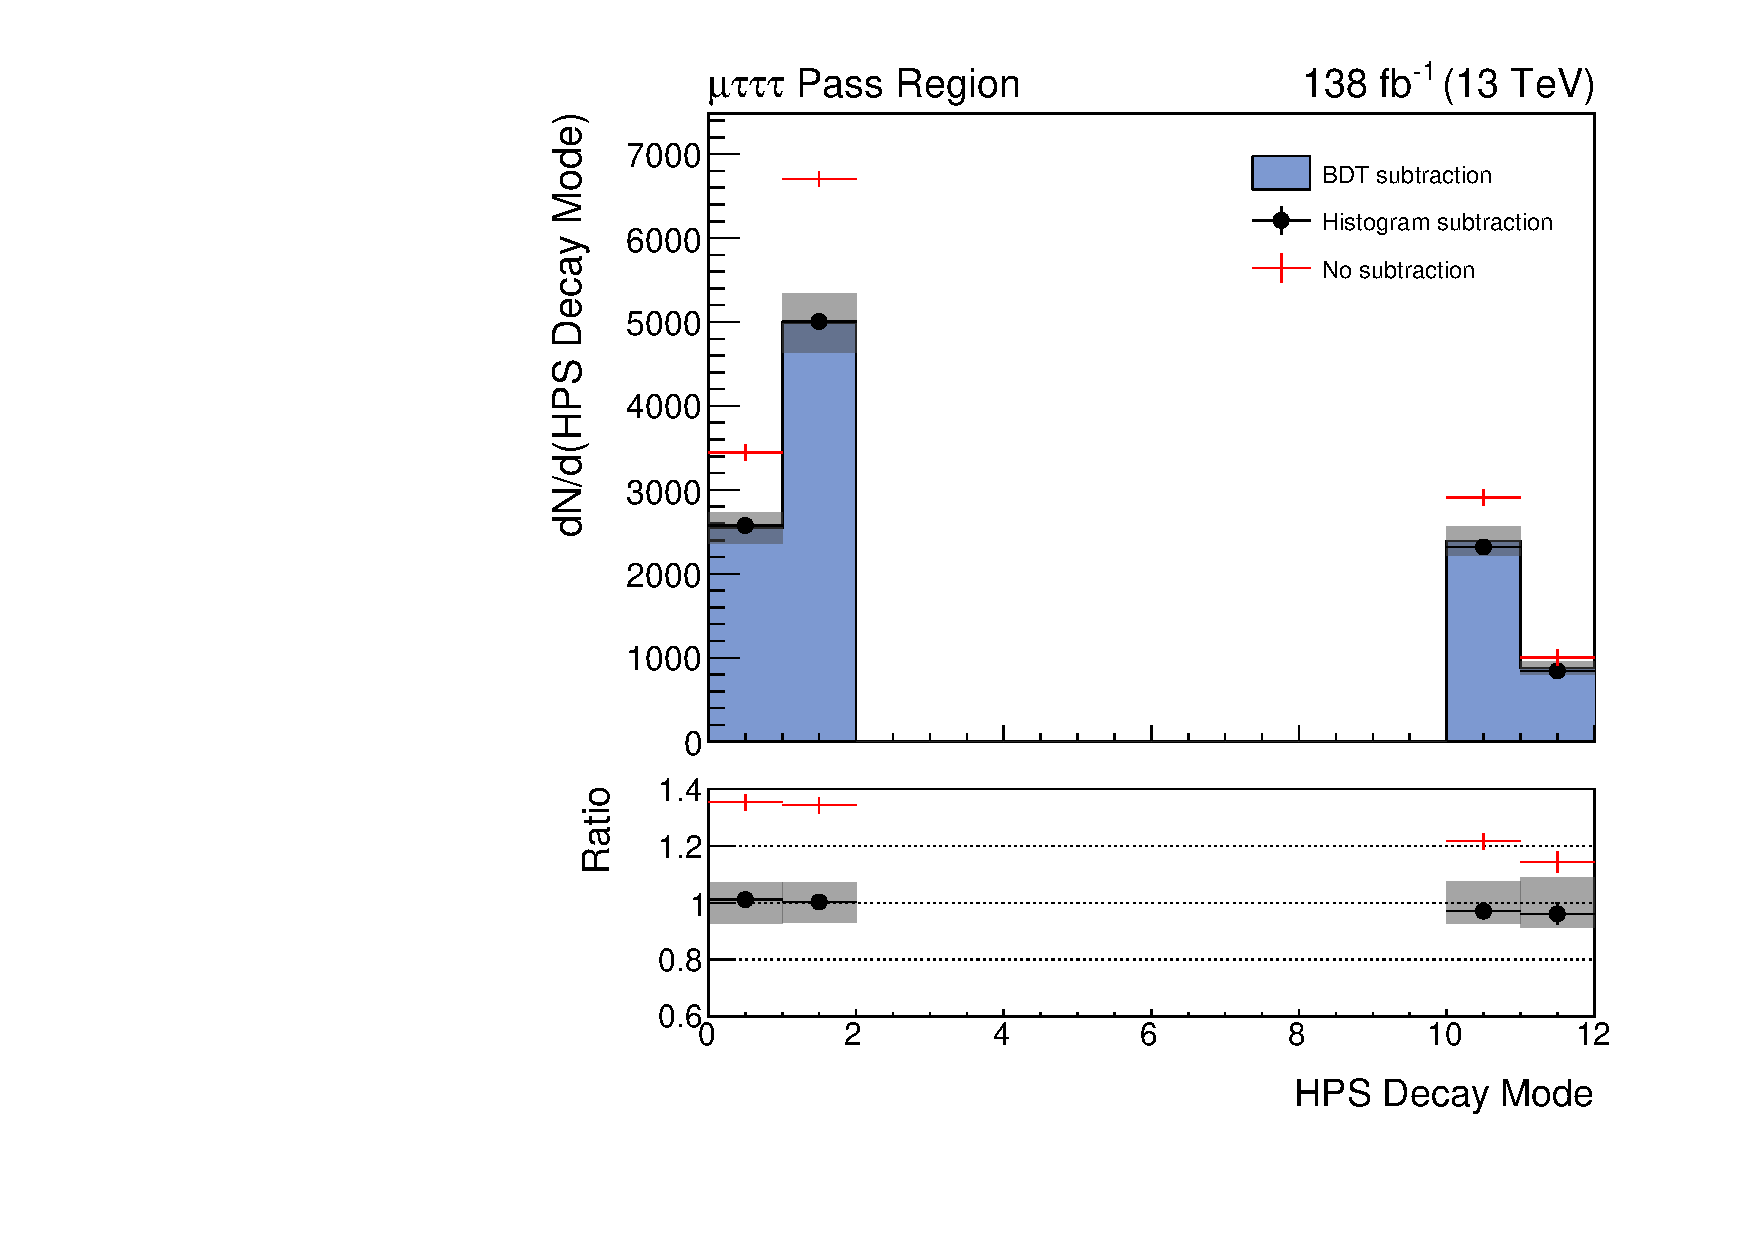
\includegraphics[width=0.45\textwidth]{Figures/subtraction_plot_tau_decay_mode_1_mttt_pass.pdf}}
    \subfloat[]{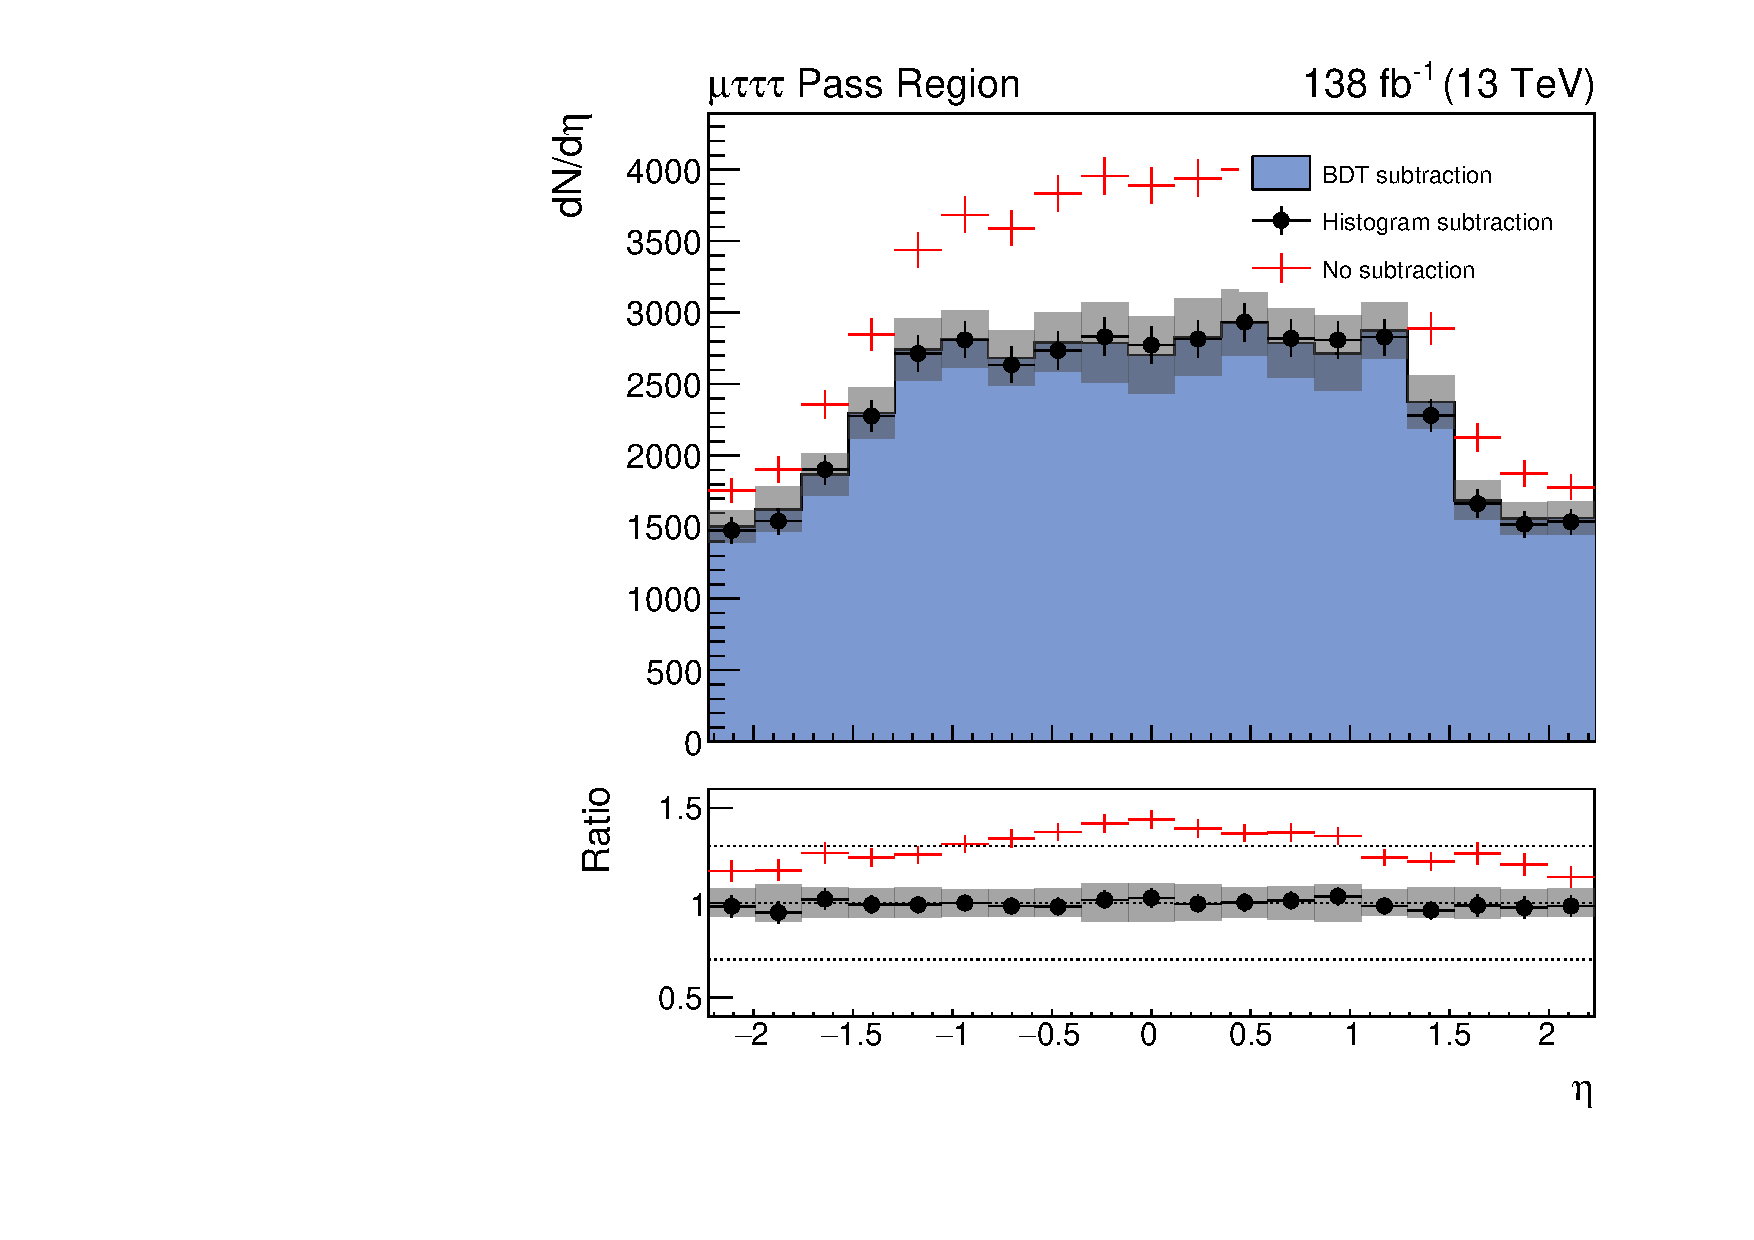
\includegraphics[width=0.45\textwidth]{Figures/subtraction_plot_eta_1_mttt_pass.pdf}}
\caption[Plots of the validation of the BDT subtraction method.]{Comparison of histograms produced via the BDT subtraction method to histogram subtraction. Also shown is the histogram produced when no subtraction is performed. The uncertainty bands contain statistical uncertainties and uncertainties from on the non-closure of the method. This shown for four of the fitted variable: $\tauh$-$\pT$, the ratio of $\tauh$-$\pT$ to jet-$\pT$, the $\tauh$ HPS decay mode and the $\tauh$-$\eta$.}
\label{fig:4tau_ff_subtraction}
\end{figure}

\subsection{Fitting}

These subtracted datasets are then randomly split 50:50 into train and test datasets and only the train dataset is fit. 
The \ac{BDT} reweighter has a number of hyperparameters and these are tuned with a scan optimising the Kolmogorov-Smirnov test~\cite{16e7f618-c06b-3d10-8705-1086b218d827} on the test dataset in each channel separately.
Final models are then produced that can optimally model \jtth candidates for all fitted variables. 
Examples of the $\FF$ derived in the $\mu\tauh\tauh\tauh$ channel are shown in Figure~\ref{fig:4tau_ff_reweights}. \\

\begin{figure}[!hbtp]
\centering
    \subfloat[]{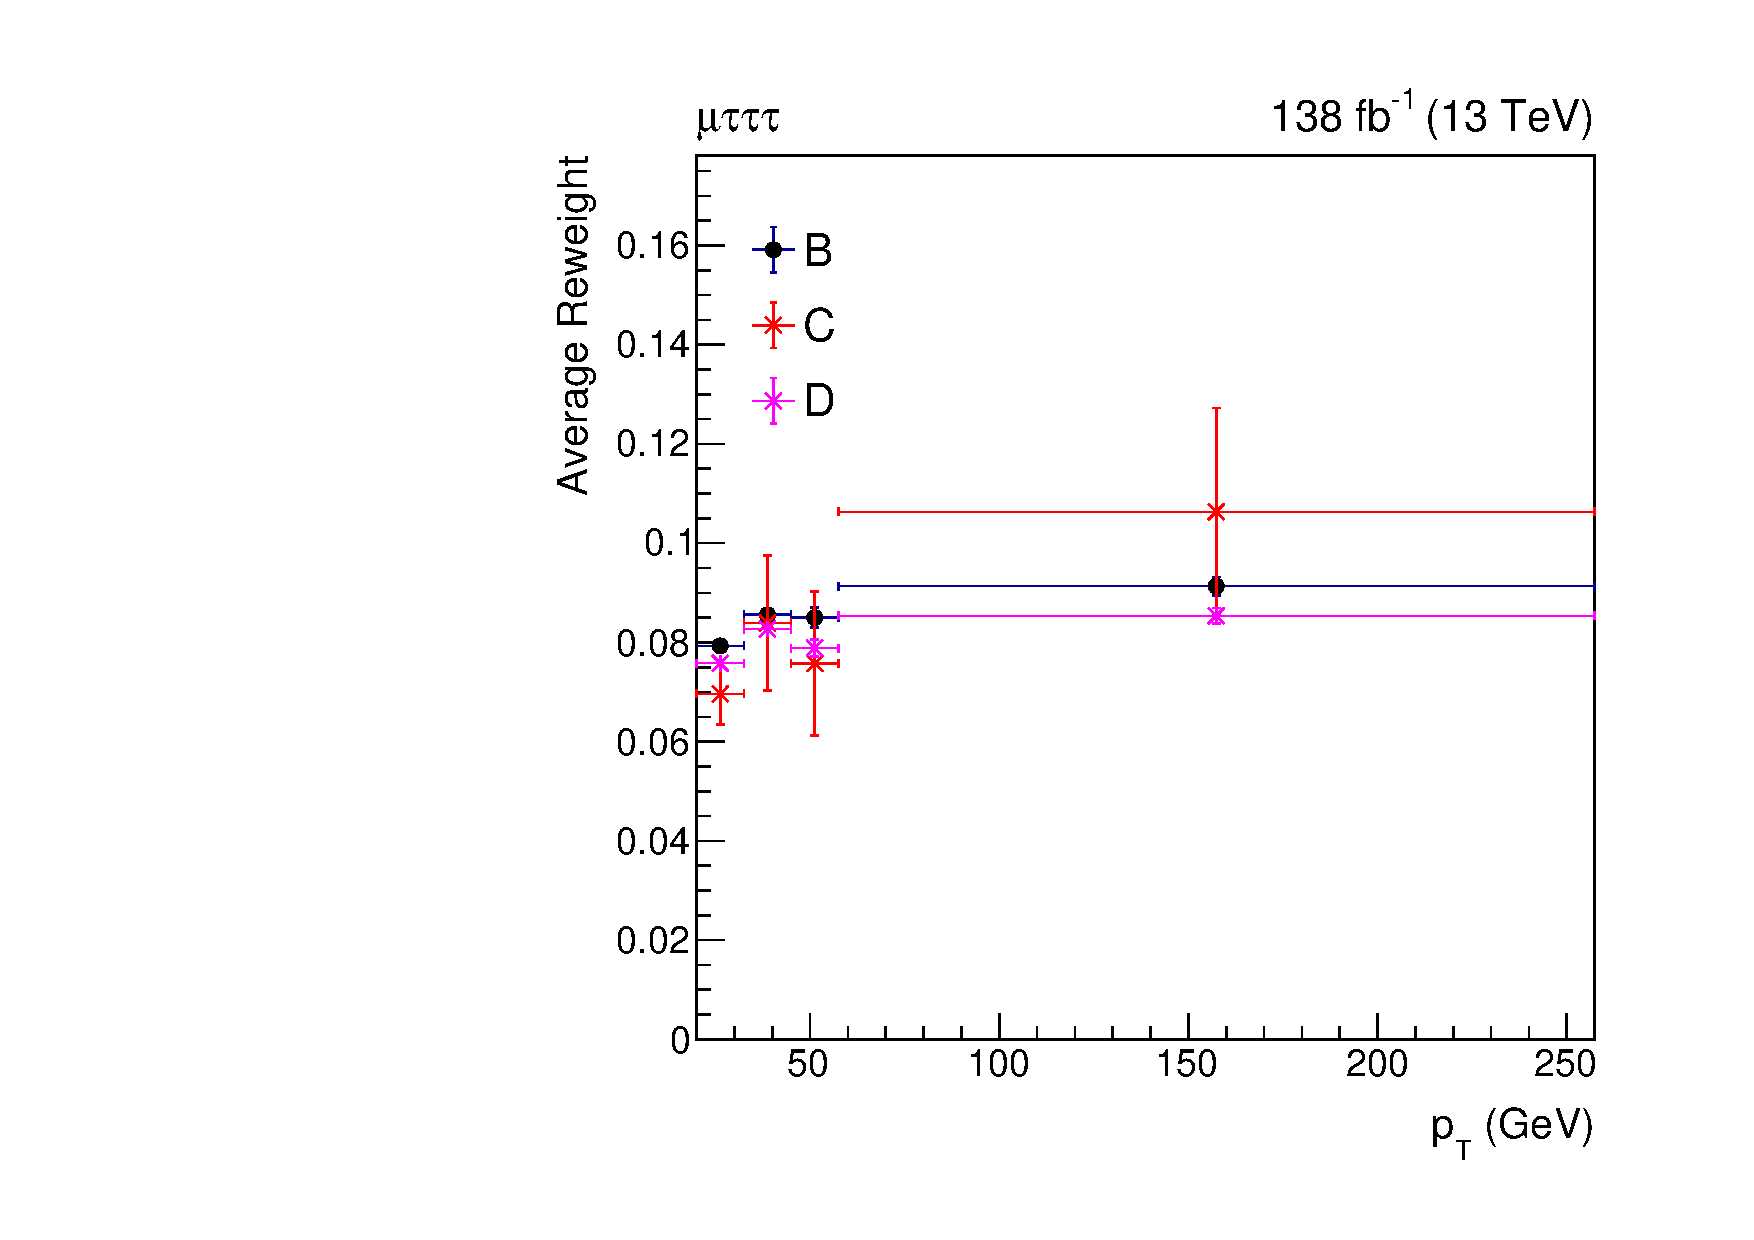
\includegraphics[width=0.45\textwidth]{Figures/reweight_ave_plot_pt_1_all_mttt_all_years.pdf}}
    \subfloat[]{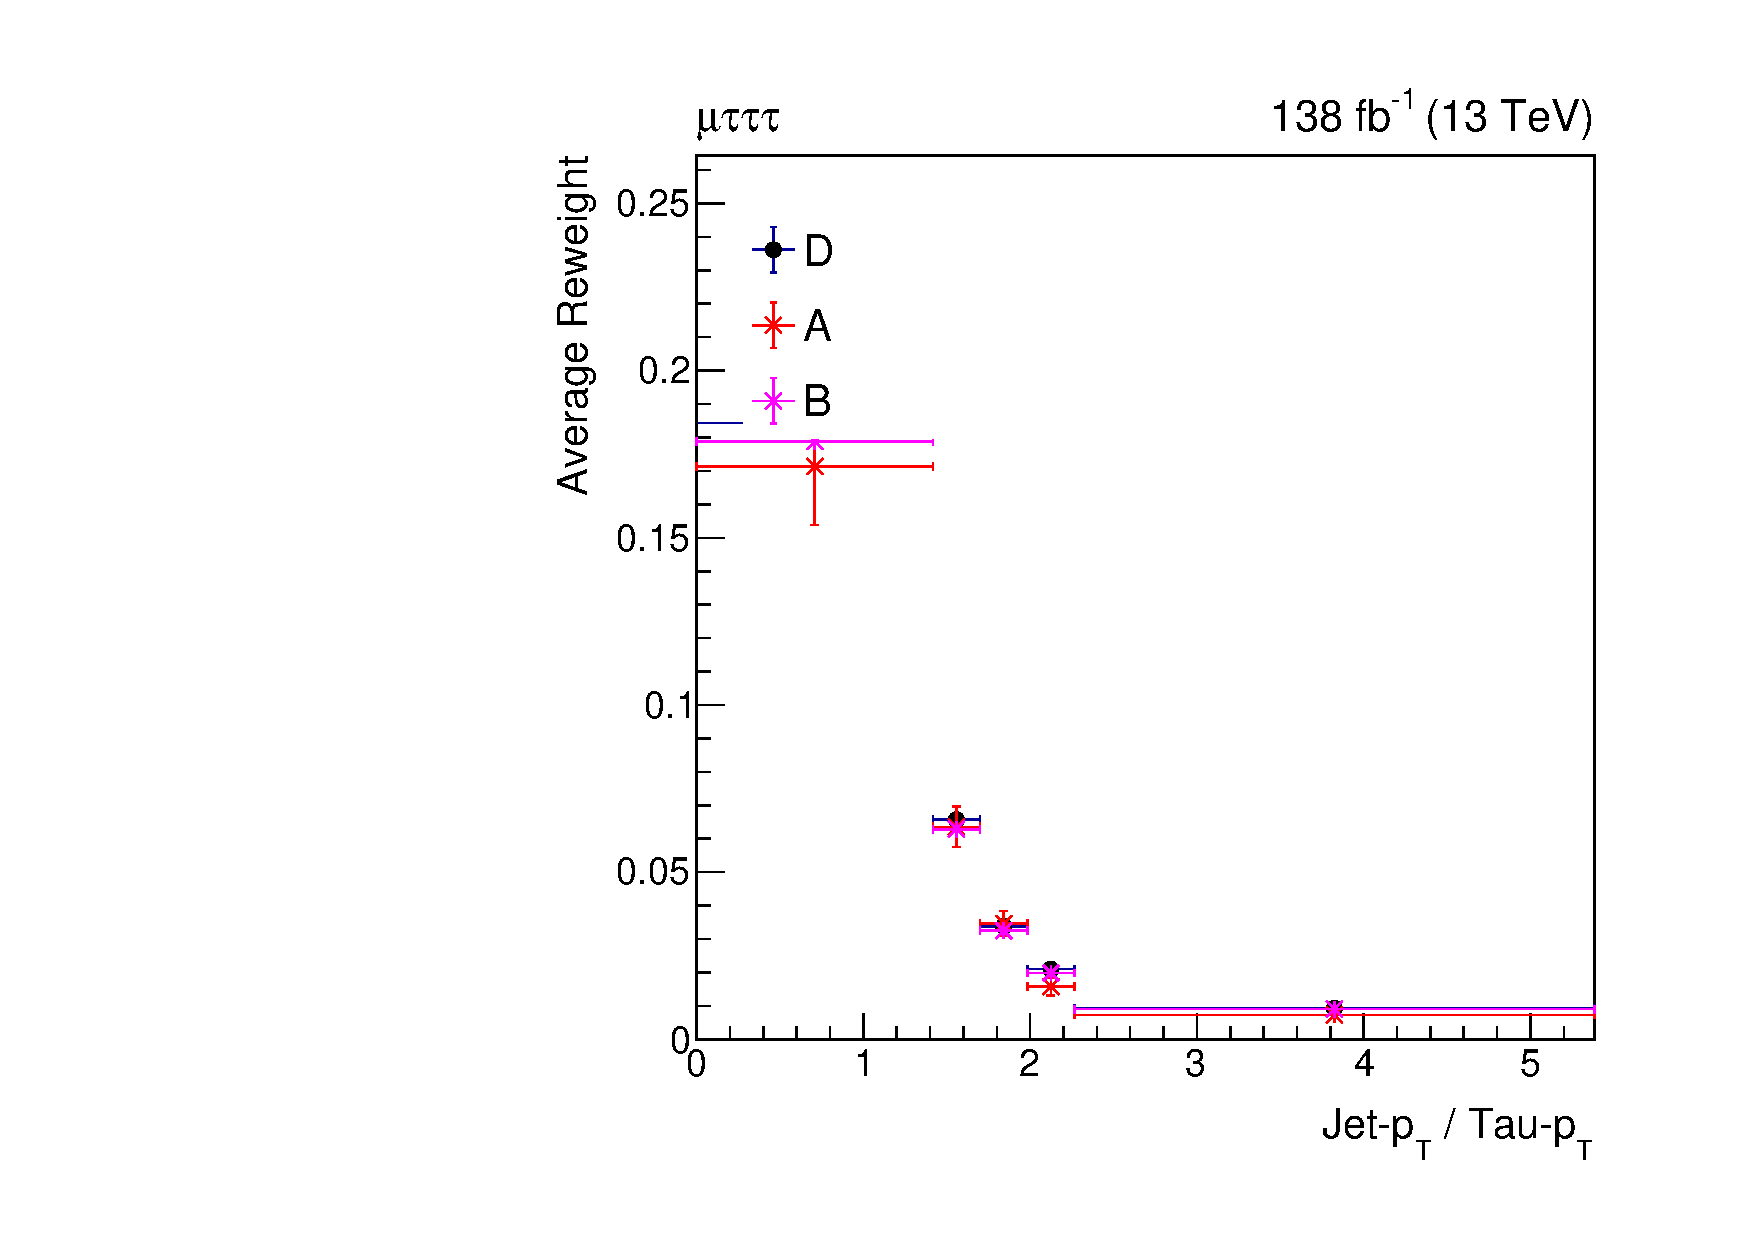
\includegraphics[width=0.45\textwidth]{Figures/reweight_ave_plot_jet_pt_1_divide_pt_1_all_mttt_all_years.pdf}} \\
    \subfloat[]{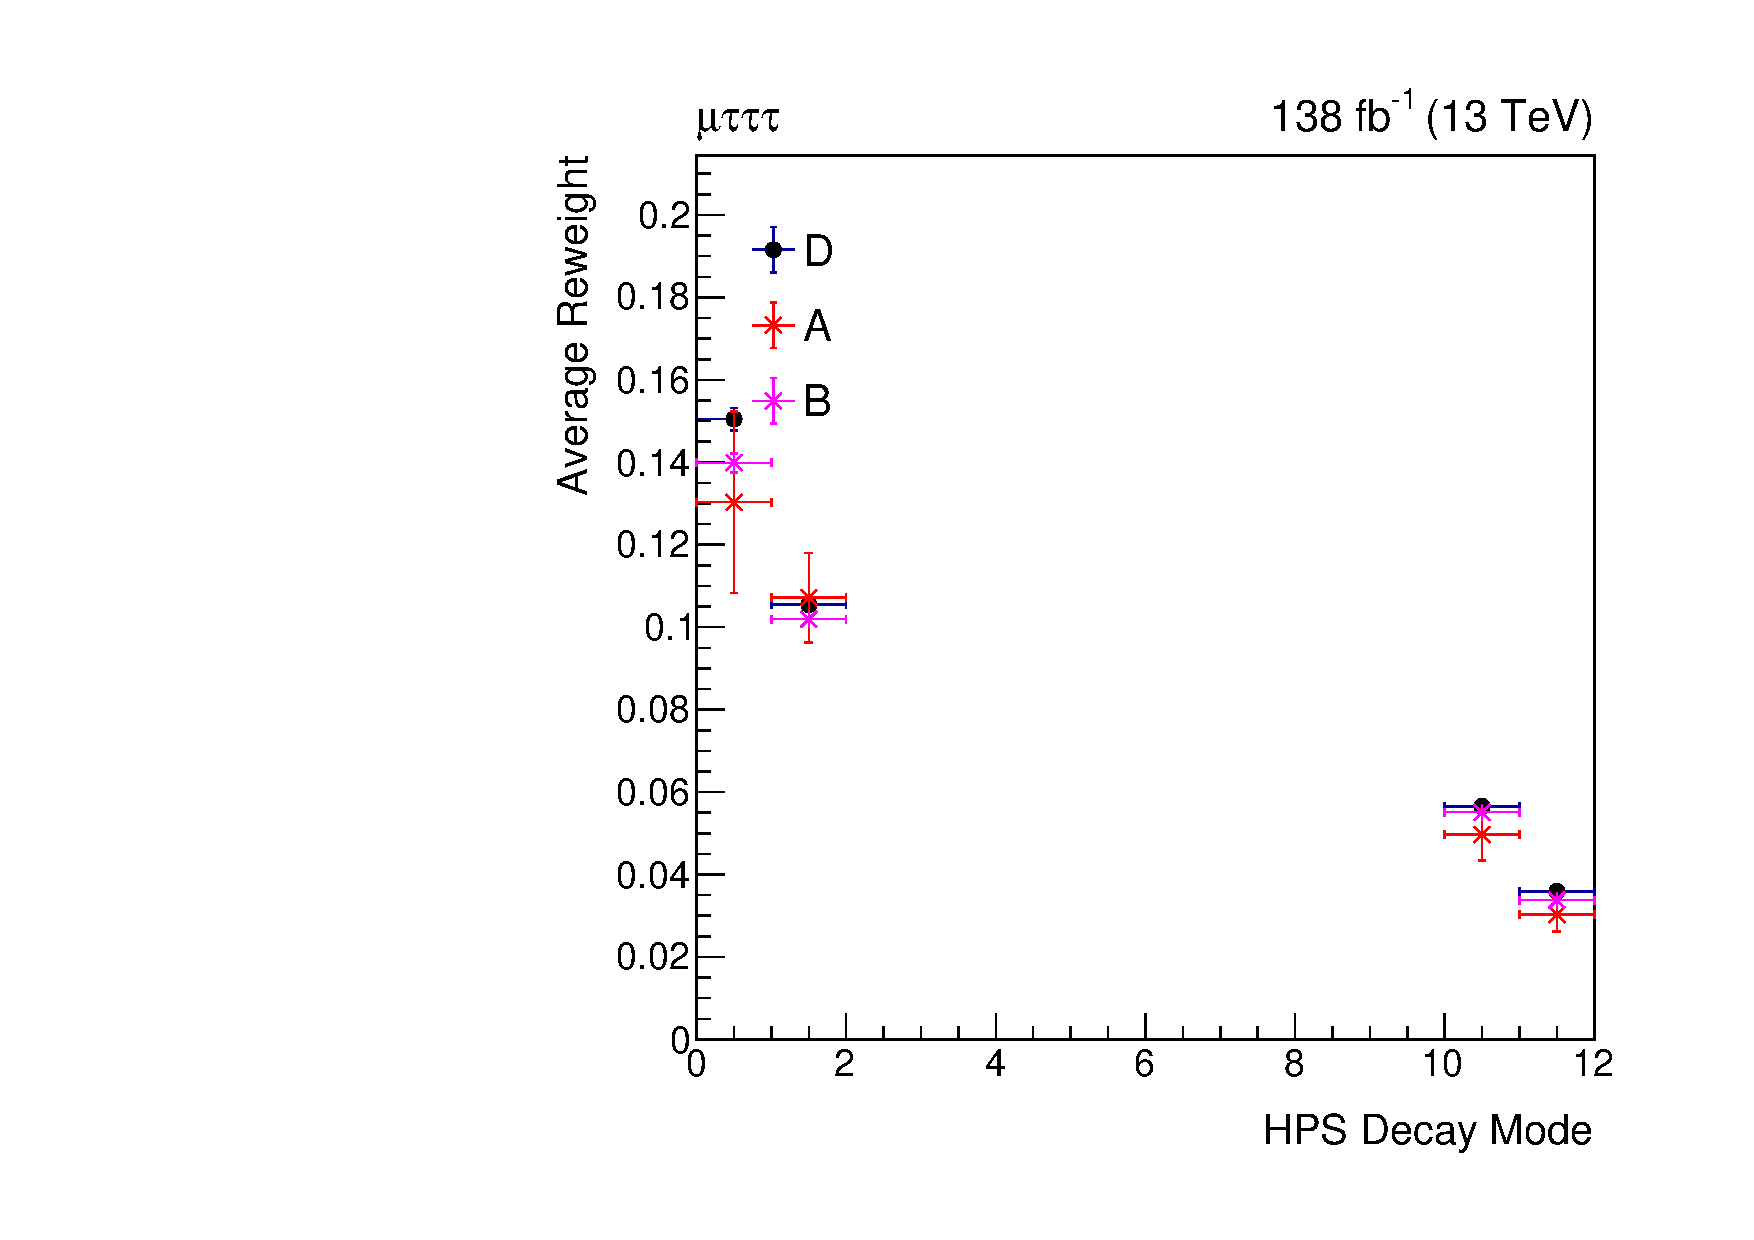
\includegraphics[width=0.45\textwidth]{Figures/reweight_ave_plot_tau_decay_mode_1_all_mttt_all_years.pdf}}
    \subfloat[]{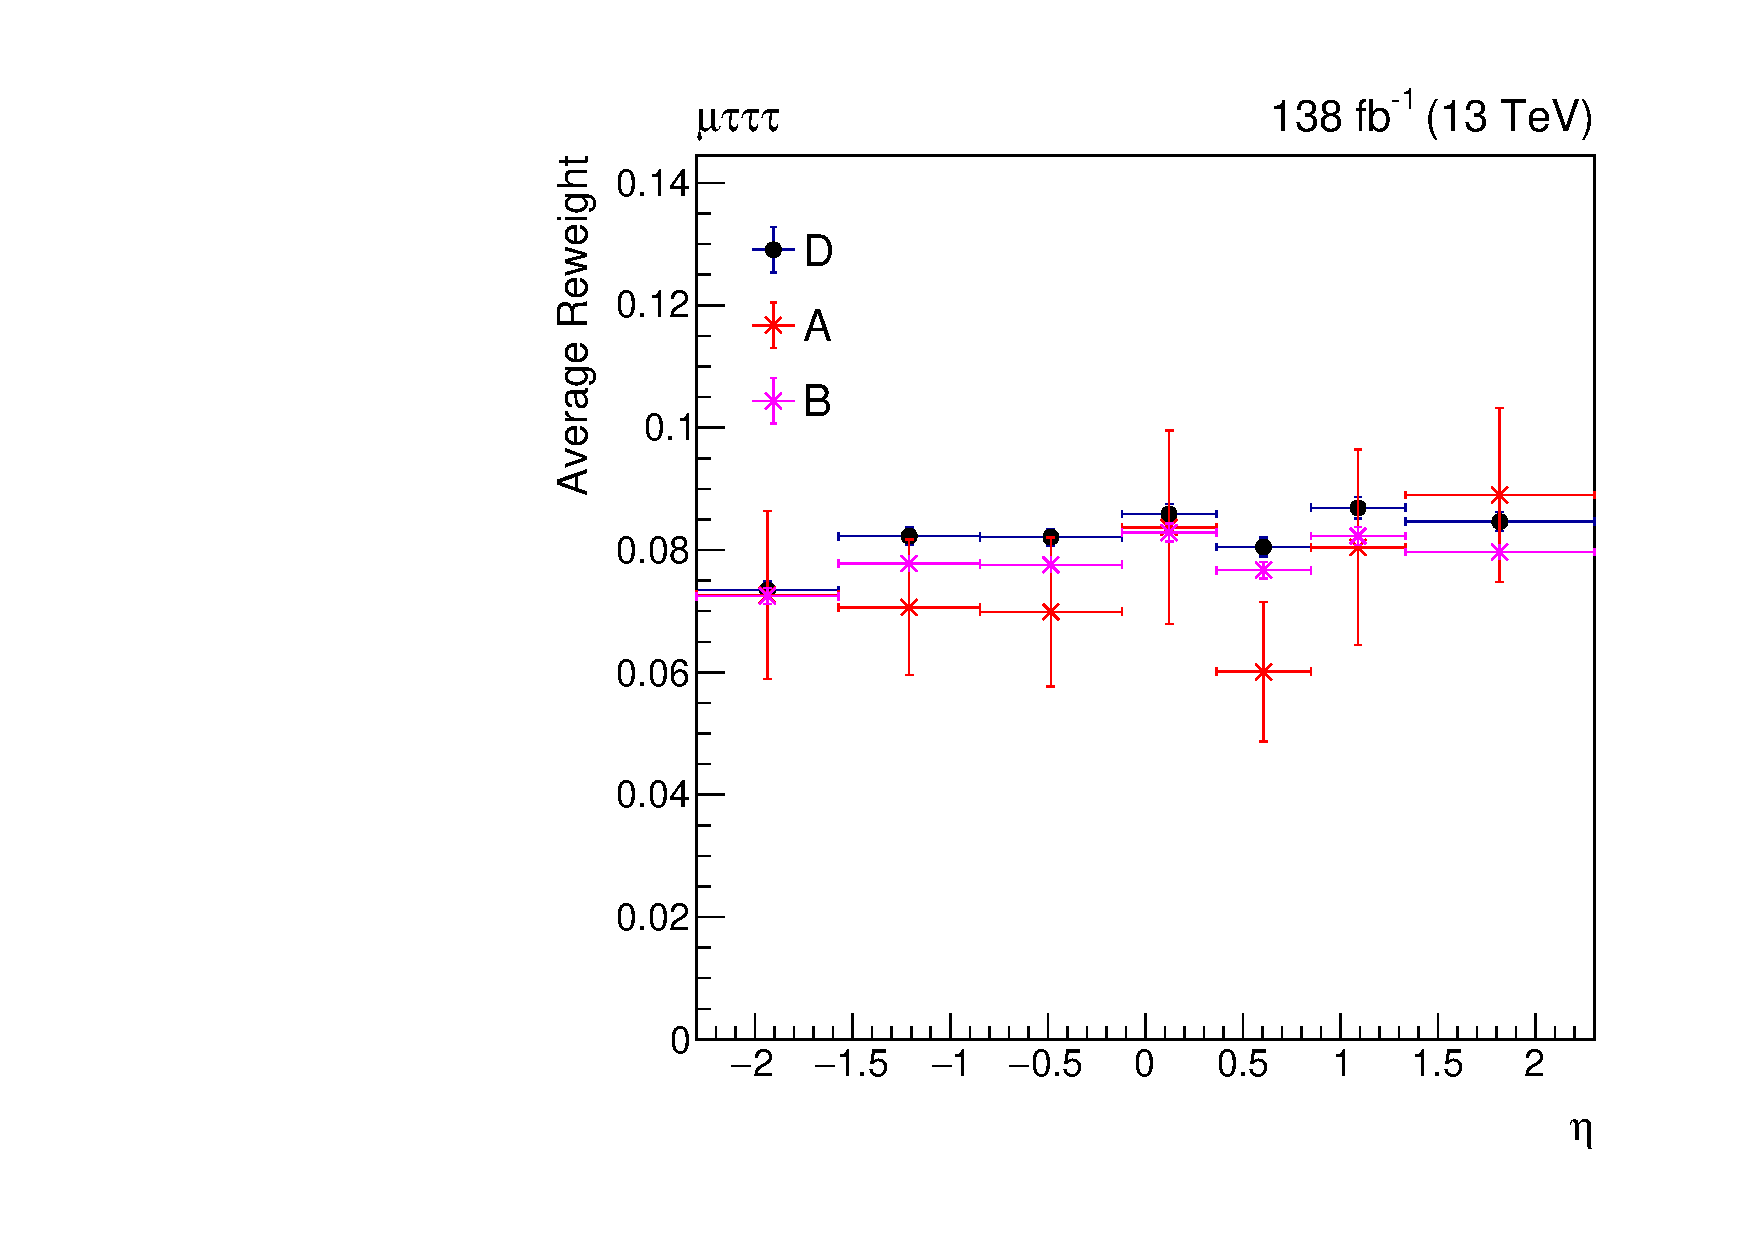
\includegraphics[width=0.45\textwidth]{Figures/reweight_ave_plot_eta_1_all_mttt_all_years.pdf}}
\caption[Plots of the average fake factors calculated.]{Average fake factors (reweights) calculated by the BDT reweighting method shown individually in regions A, B and D as defined in Figure~\ref{fig:ff_schematic}. The is shown for four of the fitted variable: $\tauh$-$\pT$, the ratio of $\tauh$-$\pT$ to jet-$\pT$, the $\tauh$ HPS decay mode and the $\tauh$-$\eta$.}
\label{fig:4tau_ff_reweights}
\end{figure}

An uncertainty is placed on the performance of this algorithm.
This is again calculated by drawing each variable into a histogram and comparing the histograms from reweighted events with the alternative $\tauh$ identification selections to the events with the nominal $\tauh$ identification in all of the fitted regions simultaneously.
Plots showing the closure of this method in the $\mu\tauh\tauh\tauh$ channel, accompanied by this uncertainty, are shown in Figure~\ref{fig:4tau_ff_closure}. \\

\begin{figure}[!hbtp]
\centering
    \subfloat[]{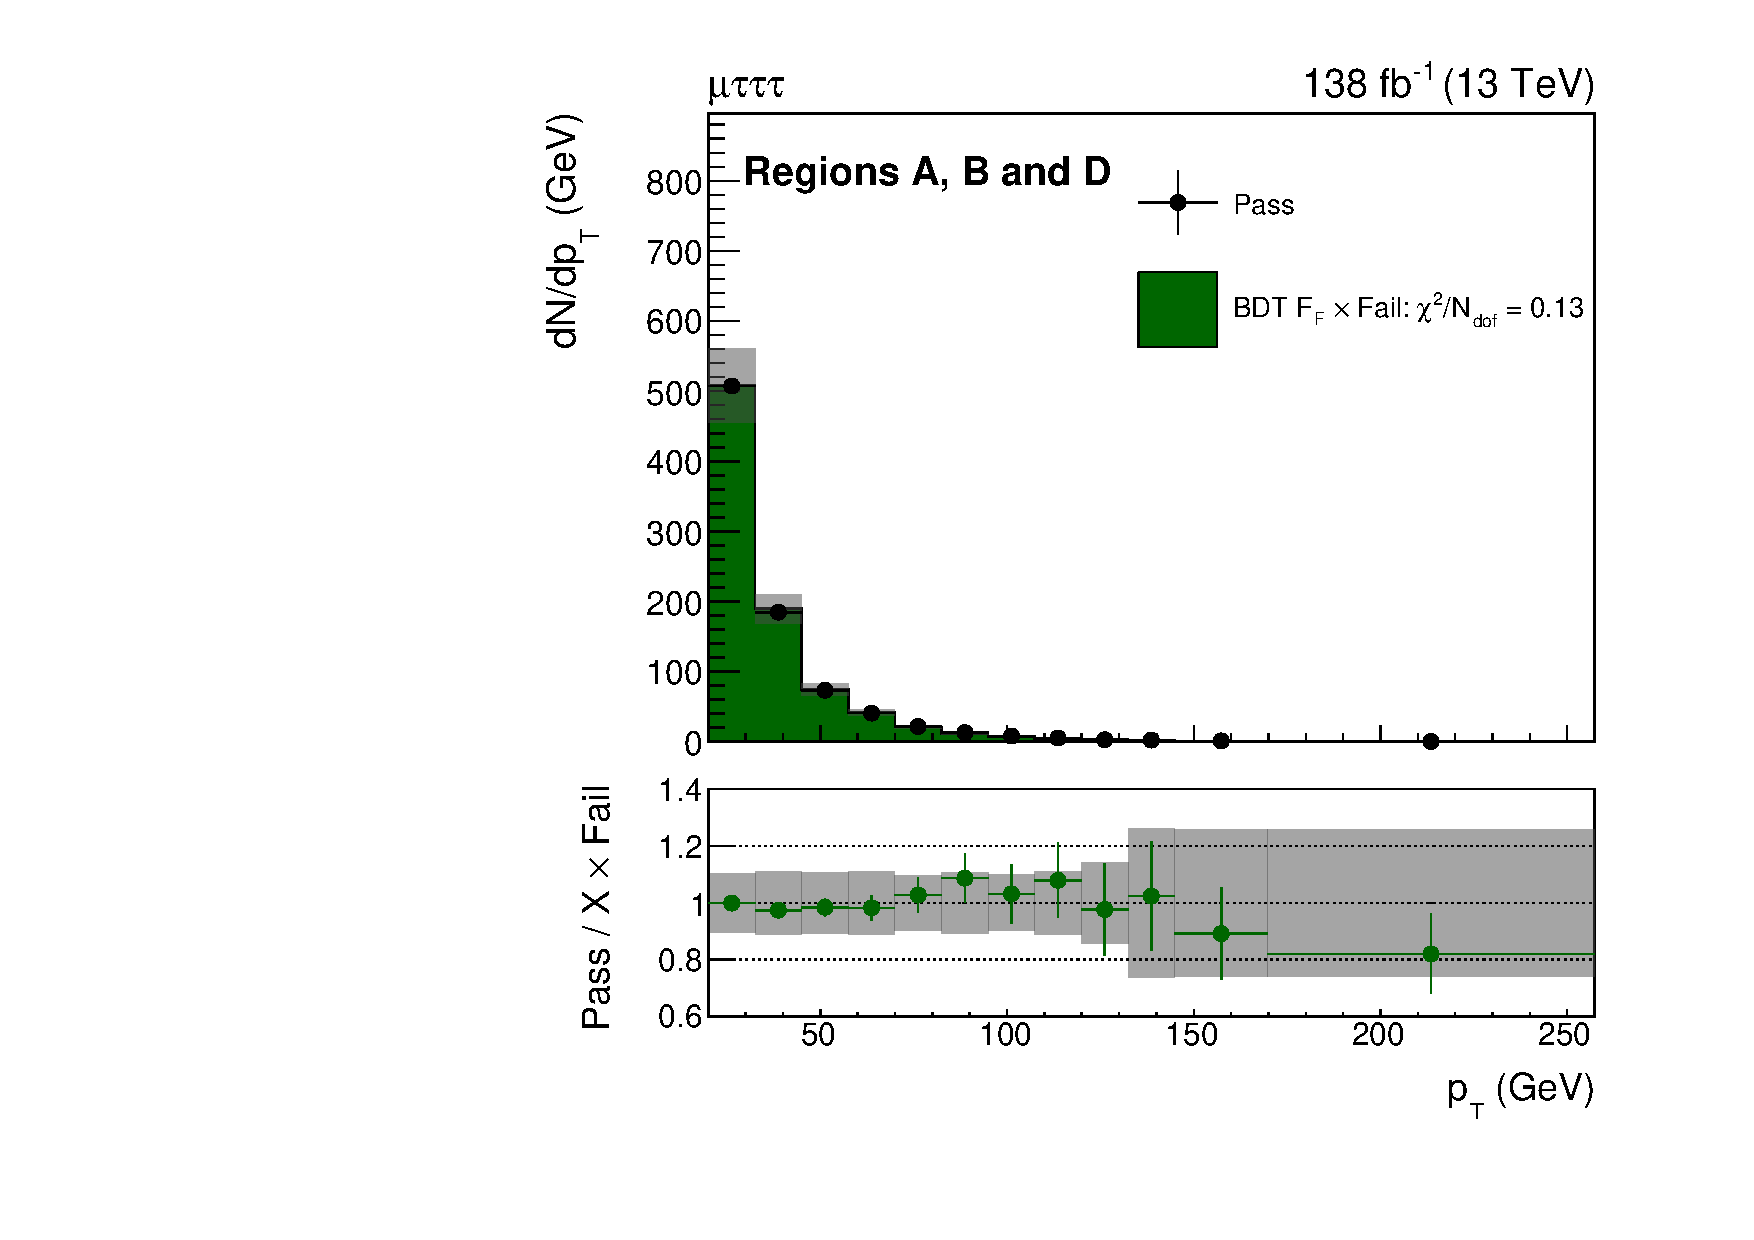
\includegraphics[width=0.45\textwidth]{Figures/closure_plot_pt_1_all_mttt_all_years_all.pdf}}
    \subfloat[]{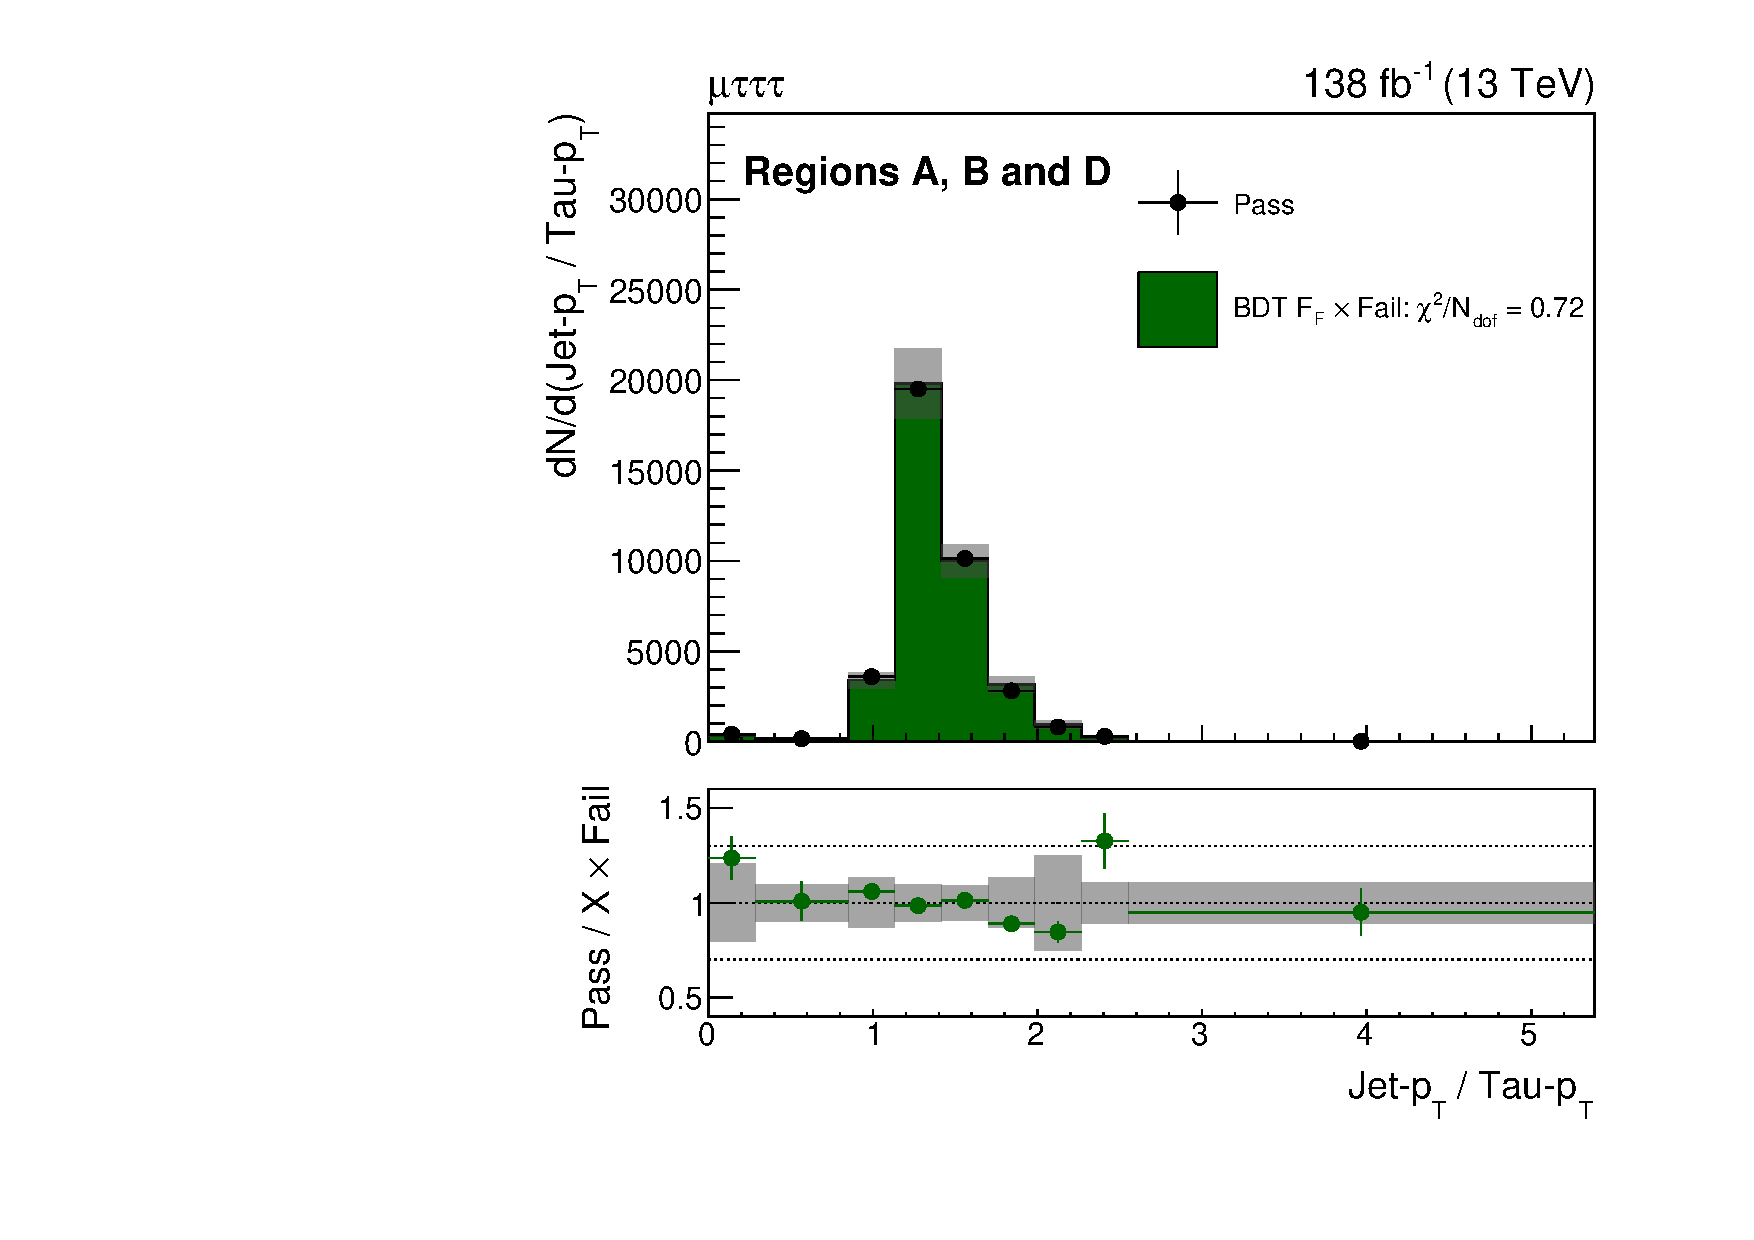
\includegraphics[width=0.45\textwidth]{Figures/closure_plot_jet_pt_1_divide_pt_1_all_mttt_all_years_all.pdf}} \\
    \subfloat[]{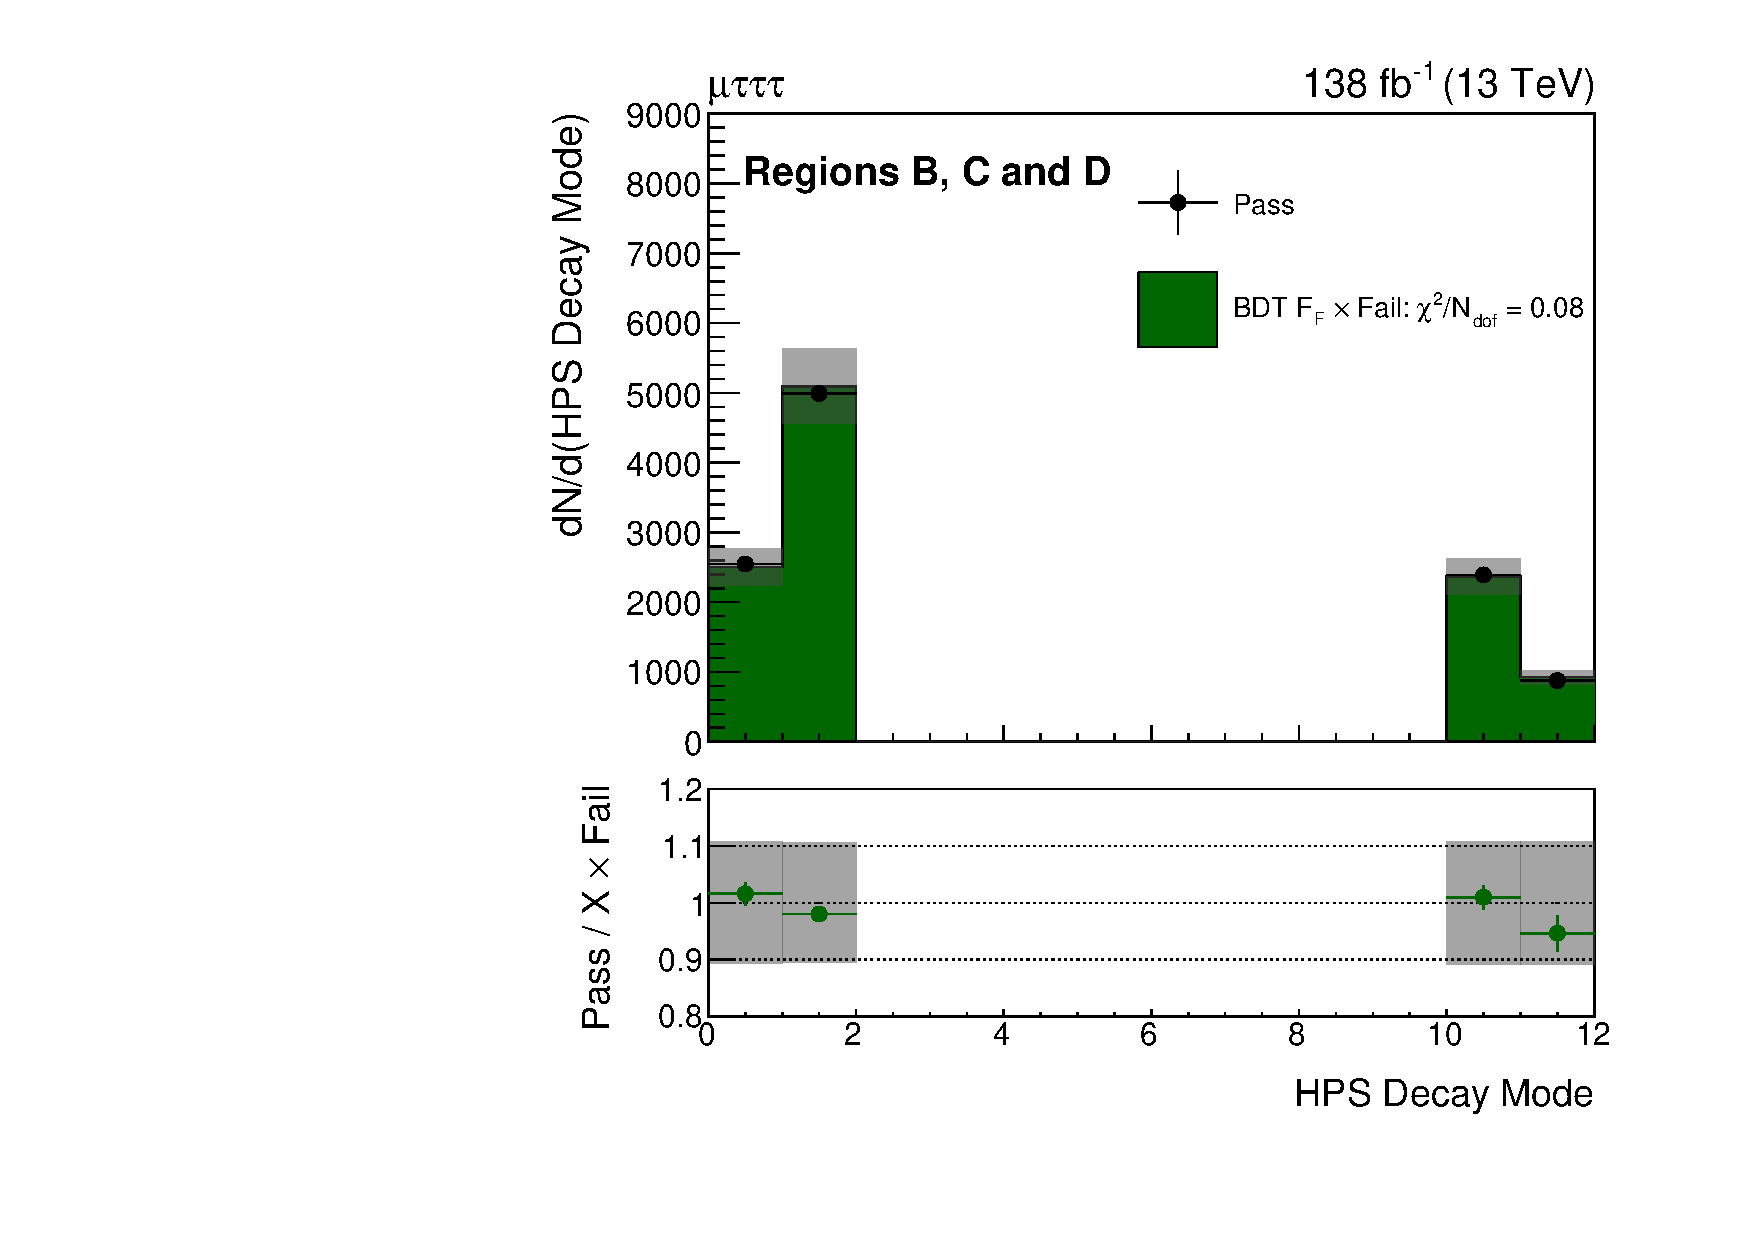
\includegraphics[width=0.45\textwidth]{Figures/closure_plot_tau_decay_mode_1_all_mttt_all_years_all.pdf}}
    \subfloat[]{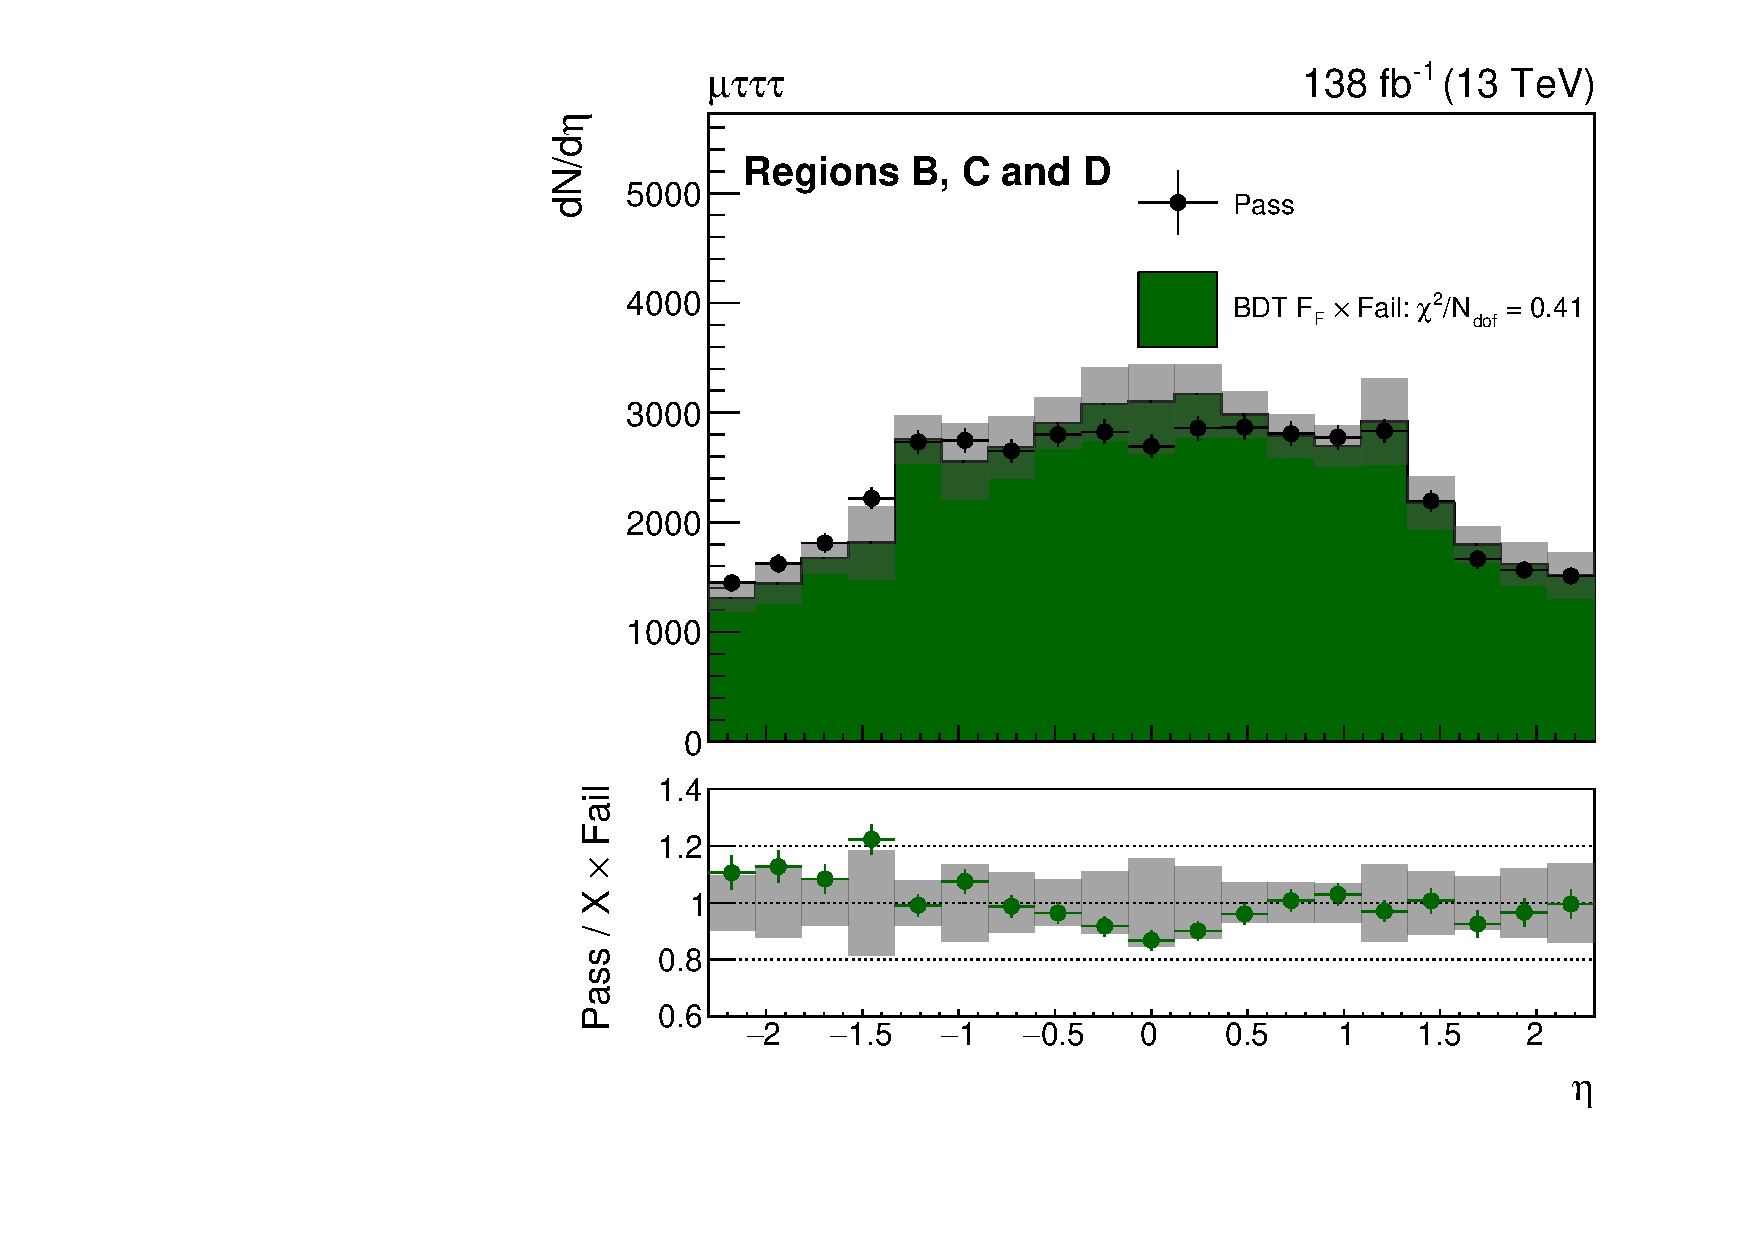
\includegraphics[width=0.45\textwidth]{Figures/closure_plot_eta_1_all_mttt_all_years_all.pdf}}
\caption[Plots of the validation of the ML fake factor fits.]{Comparison of histograms produced using the fake factors applied to the fitted fail $\tauh$ identification region compared to the fitted pass $\tauh$ identification region. The uncertainty bands contain statistical uncertainties and uncertainties derived from the non-closure of the method. The is shown for three of the fitted variable: $\tauh$-$\pT$, the ratio of $\tauh$-$\pT$ to jet-$\pT$, the $\tauh$ HPS decay mode and the $\tauh$-$\eta$. The $\chi^2$ divided by the number of degrees of freedom between the two histograms is also shown.}
\label{fig:4tau_ff_closure}
\end{figure}

\subsection{Applying fake factors}

Fake factors, $F_{F}^{i}$, have now been calculated for each $\tauh$ candidate, $i$, in the event and uncertainties determined on each weight. 
However, it is difficult to generate a full description of any number of \jtth objects in an event.
Taking channels with two $\tauh$ candidates as the simplest example, if the \jtth background is determined purely off the leading $\tauh$ candidate, then events where the leading $\tauh$ is genuine and the sub-leading $\tauh$ is a jet, are missed.
Similarly, the situation can be flipped if the sub-leading $\tauh$ is chosen to determine the \jtth fake background.
A third option can be tried where both $\tauh$ candidates are used to determine the background.
However, this will only model events where both $\tauh$ candidates are jets and not where there is a single \jtth object. 
It is seen that if the first two attempts at calculating this background from individual candidates are added and the contribution from both $\tauh$ candidates is subtracted, all possible numbers of \jtth objects in the event are accounted for, as shown in Table~\ref{tab:apply_ff}. \\

\begin{table}[H]
\centering
\begin{tabular}{|l|ccc|}
\hline
Region    & $\tauh^1 (\tau) \tauh^2 (j)$ & $\tauh^1 (j) \tauh^2 (\tau)$ & $\tauh^1 (j) \tauh^2 (j)$ \\
\hline
\hline
$R_{1}$ (from $\tauh^1$)     & 0                            & 1                            & 1                         \\
$R_{2}$ (from $\tauh^2$)     & 1                            & 0                            & 1                         \\
$R_{12}$ (from both)         & 0                            & 0                            & 1                         \\
\hline
$R_{1} +R_{2} - R_{12}$      & 1                            & 1                            & 1       \\                  
\hline
\end{tabular}
\caption[Regions modelled by the fake factor method using different $\tauh$ objects.]{Regions modelled by the fake factor method when using the leading $\tauh$ ($\tauh^1$), the sub-leading $\tauh$ ($\tauh^2$) and both, to model the jet $\rightarrow \tauh$ background and whether that specific object is a genuine $\tau$ lepton ($\tau$) or a jet ($j$). Also shown is a combination of three regions to fully model all possible combinations. }
\label{tab:apply_ff}
\end{table}

This logic is extended to all channels with one exception.
The $\tau_h \tau_h \tau_h \tau_h$ channel application region would have overlap with the $\tau_h \tau_h \tau_h$ signal region using this common method. 
Therefore, the formula is adjusted to avoid this region.
If the overlapped regions are removed from the equation, the scale of the triple and quadruple regions needed to be adjusted to account for this.
The caveat to this is that events where there is only one \jtth candidate are not accounted for.
As the majority of the background events in this channel come from \ac{QCD} with many \jtth candidates, this contribution is deemed negligible.
The formulae for the total \jtth backgrounds in each channel are shown below. \\

\begin{enumerate}[i)]
\item $\mu\mu\tauh\tauh$, $ee\tauh\tauh$ and $e\mu\tauh\tauh$
\begin{equation}
R_1 + R_2 - R_{12}
\end{equation}

\item $\mu\tauh\tauh\tauh$, $e\tauh\tauh\tauh$ and $\tauh\tauh\tauh$
\begin{equation}
R_1 + R_2 + R_3 - R_{12} - R_{13} - R_{23} + R_{234}
\end{equation}

\item $\tauh\tauh\tauh\tauh$
\begin{align}
\begin{split}
&R_{12} + R_{13} + R_{14} + R_{23} + R_{24} + R_{34} \\
&- 2(R_{123} + R_{124} + R_{134} + R_{234}) + 3R_{1234}
\end{split}
\end{align}
\end{enumerate}
 
\section{Uncertainty model}

The uncertainty model follows the schemes detailed in Section~\ref{sec:uncerts} for the statistical uncertainties and systematic uncertainties for light leptons, jets, leptons misidentified as hadronic taus, MET, luminosity and prefiring.
Updates and additions to the previous uncertainty model are shown below. \\

\subsubsection{Hadronic taus}
An improvement is made to the $\tauh$ identification uncertainty correlation scheme applied to simulated events.
The fit used to derive scale factors for the $\tauh$ \ac{MC} events consists of both statistical and systematic uncertainties.
In the previous search, the identification uncertainties were correlated across decay mode and the era of dat taking despite the statistical components of each fit begin orthogonal.
Therefore, for this search, the uncertainty scheme contains correlated and decorrelated parts across the \ac{HPS} decay mode and the era of data taking.
The double-$\tauh$ trigger uncertainties remain unchanged. \\

\subsubsection{Jets misidentified as hadronic taus}
The backgrounds with jets misidentified as $\tauh$ are estimated from data with the \ac{ML} $\FF$ method. 
There are different sources of uncertainty related to this method. 
All uncertainties are uncorrelated across decay channels, except in the $\tauh\tauh\tauh\tauh$ and $\tauh\tauh\tauh$ where the same fit is used, so uncertainties are correlated. \\

The initial uncertainties come from the removal of the non \jtth backgrounds from the fitting region and this is split into two types.
Firstly, an uncertainty is placed on the non-closure of the \ac{BDT} subtraction method, this is done by comparing the distributions in each variable fit using standard histogram subtraction with the \ac{BDT} subtraction method, and the largest shift is taken for each event. This is done separately in the pass and fail $\tauh$ identification regions.
The second uncertainty to do with purifying the fitting region is motivated by any \ac{MC} mismodelling of the non \jtth objects predicted.
This is shifted up and down by 10\%, to represent any \ac{MC} mismodelling, and the \ac{BDT} subtraction method and the reweighting are repeated with the differing datasets. \\

The second source of uncertainties comes from the \ac{BDT} reweighter fit.
In a similar way to the subtraction method, an uncertainty is placed on the non-closure of the fit, comparing reweighted events in the fail $\tauh$ identification region to the pass $\tauh$ identification region.
Further uncertainties are placed on the assumption of the variables used to separate the signal region from the fitting region.
The assumption is that the fake factors would be identical no matter what combination of these variables is used.
Therefore, the uncertainties are placed by taking the largest shift when changing these variables whilst getting the output to the fit.
These are decorrelated in each combination of the separating variables.

\subsubsection{Background process-specific uncertainties}
Specific uncertainties are placed on the di-Z simulated events due to the application of K factors.
Due to the size of the differences between \ac{NNLO} and lower order predictions for the cross-sections, an uncertainty is placed on the size of these yields utilising the K factors derived.

\subsubsection{Signal process-specific uncertainties}
Parton distribution functions, $\alpha_s$ and $\mu_{R}$/$\mu_{F}$ scale variations are applied on an event-by-event basis to the signal samples.
The normalisation of these uncertainties are approximately 6\%, 1\% and 2\% respectively. 
However, these yields are factored out for the model-independent search, where the cross-section (times branching ratios) is searched for.

\section{Signal extraction}

The statistical interpretations of the results are done as described in Section~\ref{sec:sig_ext}, but with different signal scaling functions, $g$, and parameters of interest, $\mu$.
The two interpretations of the analysis, as stated at the beginning of the chapter, have different parameters of interest and scaling functions. \\

Firstly, the model-independent search uses a linear scaling function, $g(\mu)=\mu$, and a parameter of interest that represents the cross-section of the $Z^{*}\rightarrow \phi A$ multiplied by the branching fractions of $\phi\rightarrow\tau\tau$ and $\PA\rightarrow\tau\tau$.
Secondly, the interpretation in the type X \ac{2HDM} model is done by testing each point in the parameter space, whether that is $m_{A}$-$\tan\beta$ for the alignment scenario or $\cos(\beta-\alpha)$-$\tan\beta$ for scenarios of the remaining parameters. 
This is done by scaling the samples to the predicted cross-sections times branching ratios at that point in the parameter space and defining a single rate parameter that can only take the values 1 (type X \ac{2HDM}) and 0 (\ac{SM}) with $g(\mu)=\mu$.

\subsection{Postfit plots}

Figure~\ref{fig:4tau_postfit} shows the distributions of the $m_{T}^{\text{tot}}$ discriminator, after a background-only fit to data, in every bin used in the fit.
For visualisation, categories with similar event numbers in each bin are displayed on the same plot.
A stacked background of events is shown, separated into three groups: events with 1 or more \jtth objects, events where all $\tauh$ candidates are reconstructed correctly, and the remaining events where only light leptons are misidentified as $\tauh$ and not jets.
An example signal hypothesis is also shown for a mass hypothesis of $m_A = 160$ GeV and $m_{\phi} = 200$ GeV scaled to 0.01 pb, which is approximately three times smaller than the predicted cross-section for this process. \\

There are no upward deviations of the number of events observed, that would be consistent with any mass hypotheses for the signal model searched for.
The combined results are consistent with a background-only fit to data.
Within this combined fit, individual bins and categories such as the $\emu\tauhtauh$ \texttt{SS Leptons}, have small deficits of events observed in comparison to events expected.
The background prediction yield in this category from the $\FF$ method is checked with a comparison to \ac{MC} for the non-\ac{QCD} prediction.
The background estimations are compatible when the estimation of the fraction of \ac{QCD} events from the charge inverted region is taken into account, further validating the $\FF$ background prediction in this category.


\begin{figure}[!hbtp]
\centering
    \subfloat[]{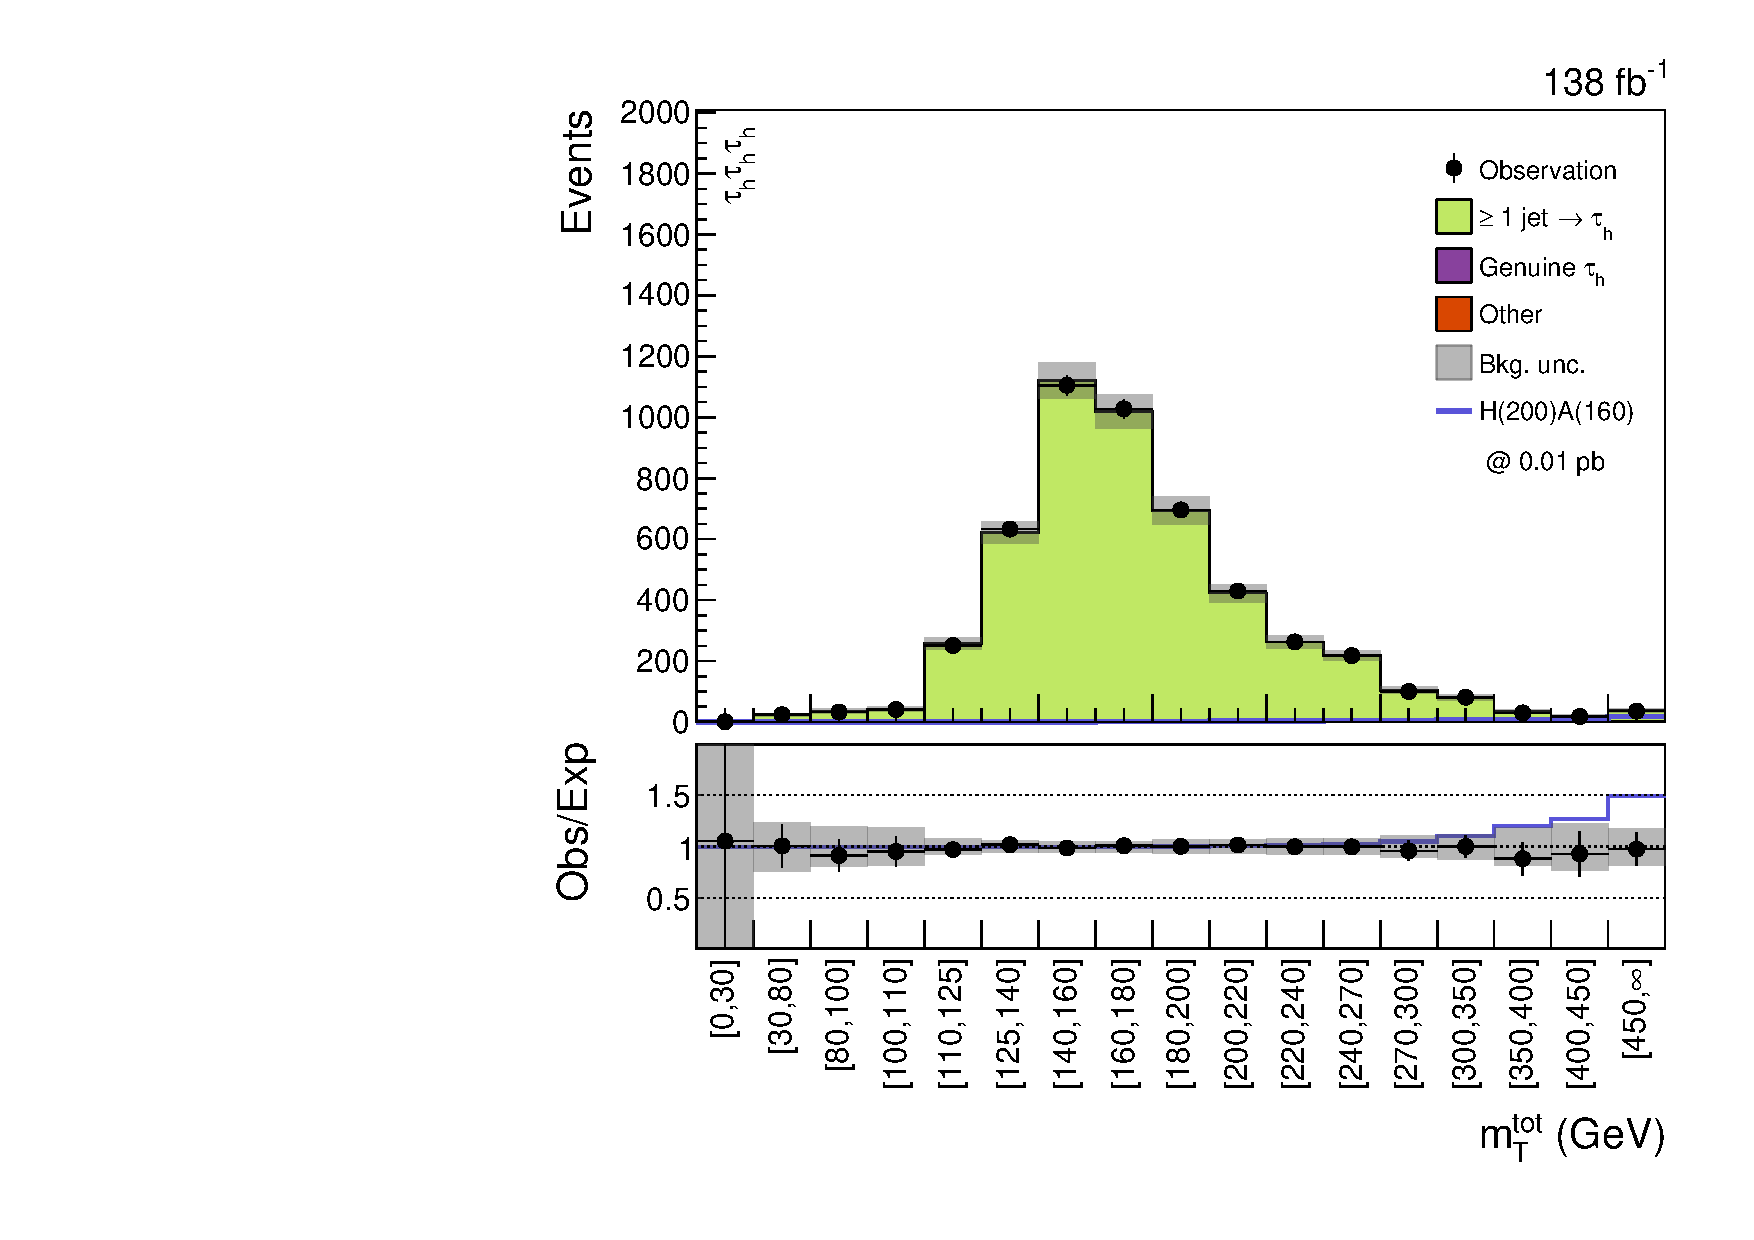
\includegraphics[width=0.5\textwidth]{Figures/postfit_plots_combined_postfit_high_stat.pdf}}
    \subfloat[]{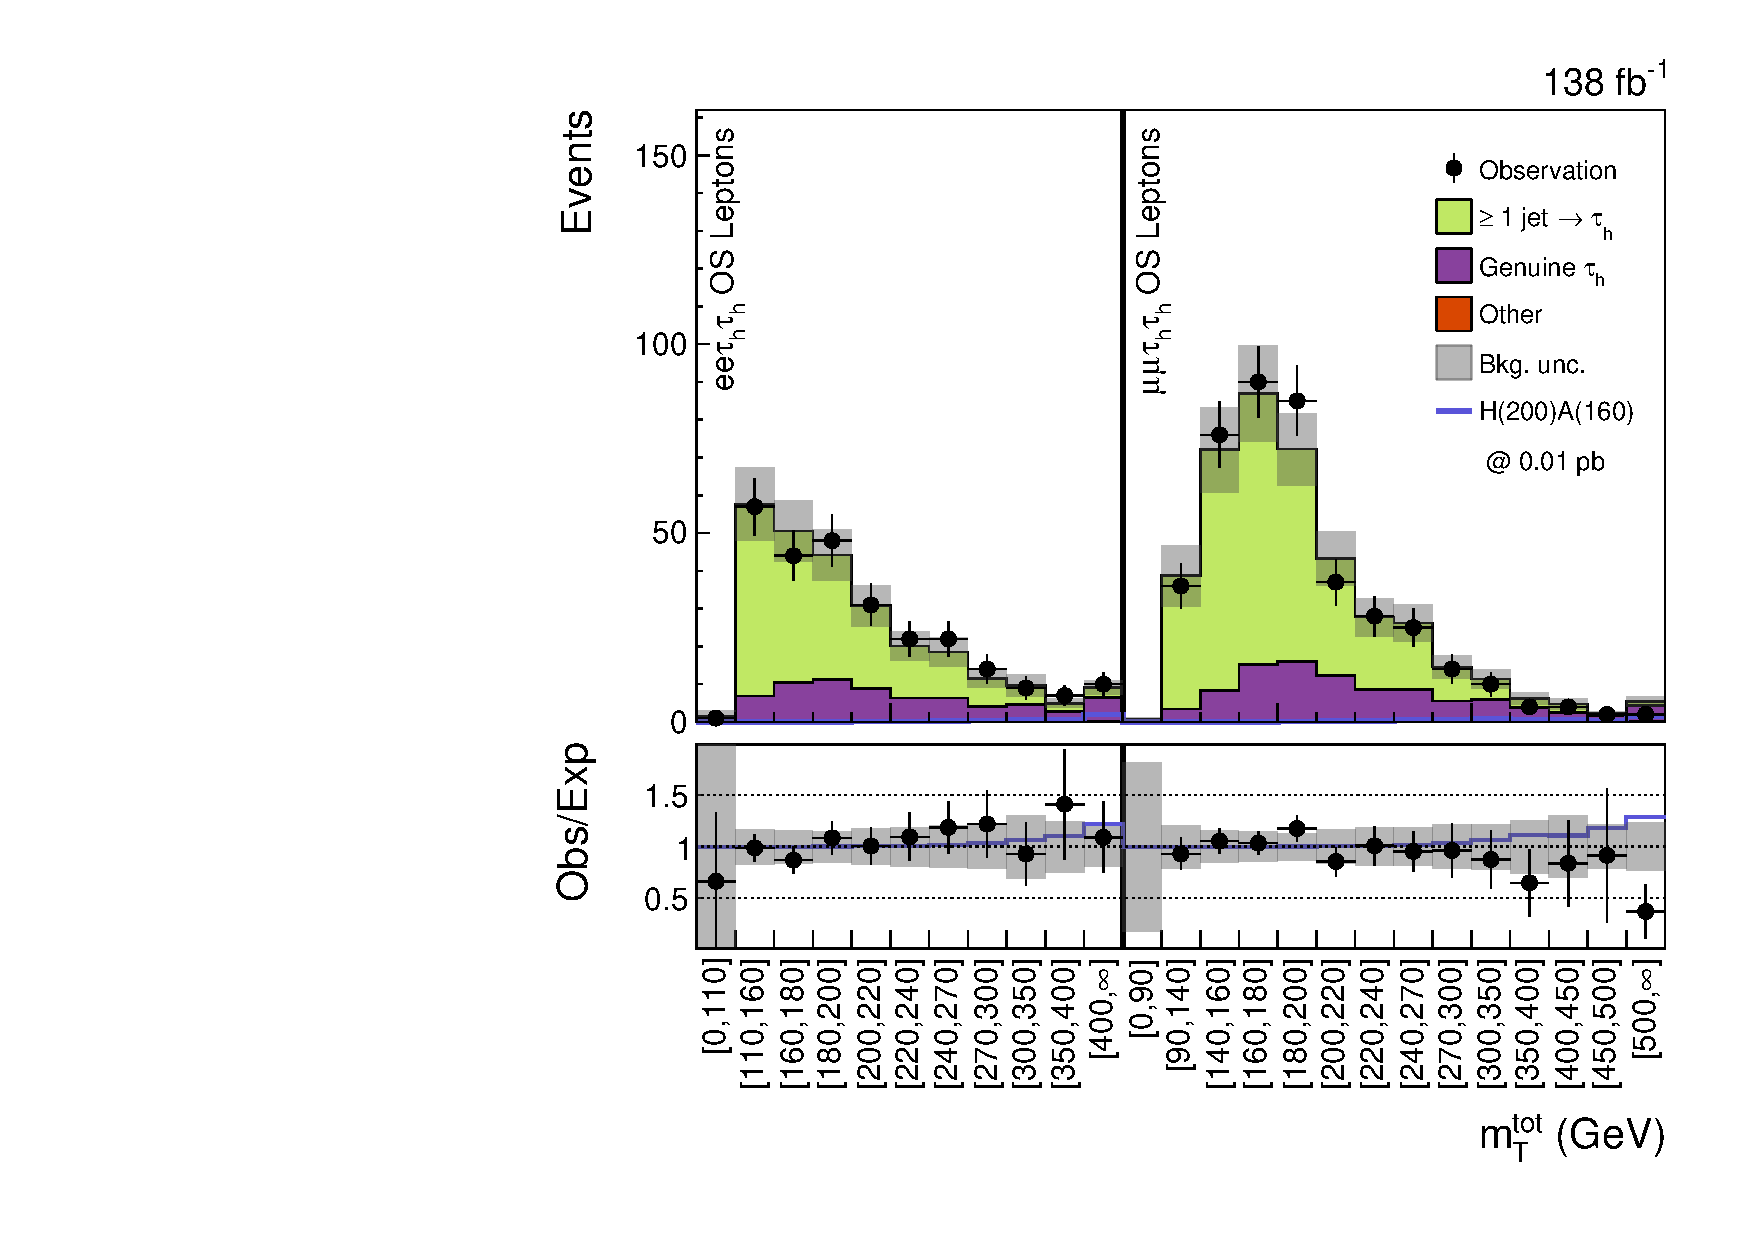
\includegraphics[width=0.5\textwidth]{Figures/postfit_plots_combined_postfit_med_stat.pdf}} \\
    \subfloat[]{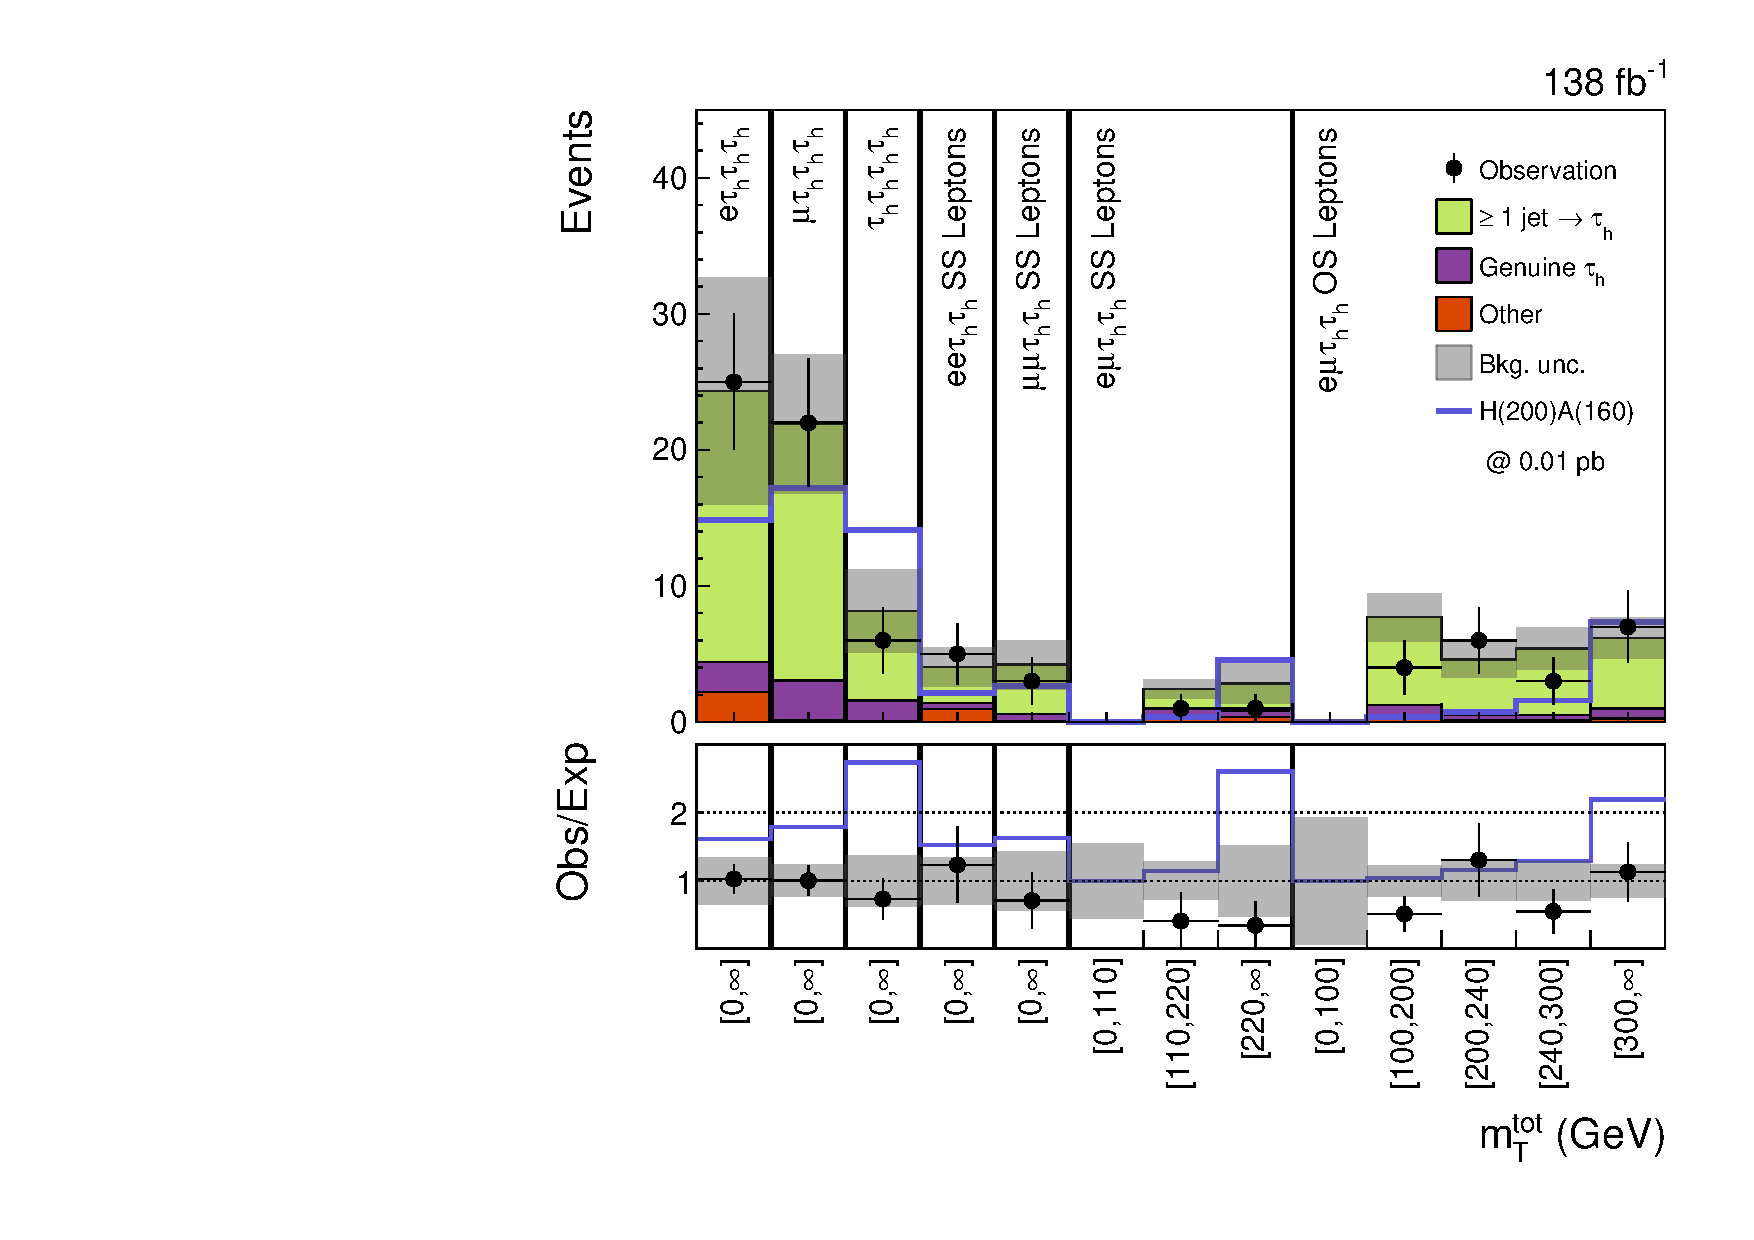
\includegraphics[width=0.5\textwidth]{Figures/postfit_plots_combined_postfit_low_stat.pdf}}
\caption[Plots of the $m_{T}^\text{tot}$ distributions in the $\tau\tau\tau\tau$ channels and categories.]{Distributions of $m_{T}^\text{tot}$ in the high (a), medium (b) and low (c) statistic categories. As the bin sizes vary drastically between channels, the bin sizes are kept constant and the bin intervals are shown on the x-axis. The high statistic categories consist of only the $\tauh\tauh\tauh$ channel, the medium statistic categories include the $ee\tauhtauh$ and $\mu\mu\tauhtauh$ \texttt{OS Leptons} categories, and the low statistic categories show the $e\tauh\tauh\tauh$, $\mu\tauh\tauh\tauh$, $\tauh\tauh\tauh\tauh$,  $ee\tauhtauh$ \texttt{SS Leptons}, $\mu\mu\tauhtauh$ \texttt{SS Leptons}, $e\mu\tauhtauh$ \texttt{SS Leptons} and $e\mu\tauhtauh$ \texttt{OS Leptons} channels and categories. The solid histograms show the stacked background predictions after a background-only fit to the data. The $m_{\phi}=200$ GeV and $m_{A}=160$ GeV signal scaled to 0.01 pb is also shown by a blue line for illustrative purposes.}
\label{fig:4tau_postfit}
\end{figure}


\section{Model-independent results}

\subsection{Limits}

95\% \ac{CL} limits are set on the cross-section for two additional neutral Higgs bosons produced via an off-shell Z boson multiplied by the branching fraction of each additional boson decaying to $\tau$ lepton pairs and are shown in Figure~\ref{fig:4tau_mi}.
To show this for all 72 mass hypotheses, the limits on higher masses of the $\PA$ boson are scaled to larger negative powers of 10, as indicated on the plot.
The observed limit falls between the lower 1 and 2$\sigma$ bands of the expected result.
This is consistent with the distributions observed in Figure~\ref{fig:4tau_postfit}, as the small deficits in sensitive channels lead to a strengthening of the limit.
The observed limit in comparison to the expected limit is relatively consistent across the signal mass range.
This is because of the degeneracy of the signal hypothesis in the sensitive category bins fit.
Therefore, the strongest constraints on different mass hypotheses mostly arise from the same bins.
The observed limits vary from 20 fb at the lowest mass hypothesis of $m_A = 60$ GeV and $m_{\phi} = 100$ GeV, to 1.4 fb at the highest mass hypothesis of $m_A = 160$ GeV and $m_{\phi} = 300$ GeV.
It is worth noting that each of the observed limits is well below the predicted cross-sections calculated and shown in Figure~\ref{fig:4tau_xs}, indicating excellent sensitivity to the type X \ac{2HDM} in the alignment scenario. \\

Figure~\ref{fig:4tau_limit_comparison} shows the effect of individual decay channels, by showing the expected 95\% \ac{CL} limit on fits to each decay channel separately for an $m_{A} = 100$ GeV scenario.
It is observed from this, that the dominant search channels, across the whole $m_{\phi}$ range, are the $\tauh\tauh\tauh\tauh$, $\mu\tauh\tauh\tauh$ and $e\mu\tauh\tauh$.
The $\tauh\tauh\tauh$ channel can significantly contribute to the combined limit at higher values of $m_{\phi}$, as the distribution of events in $m_{T}^{\text{tot}}$ peaks higher and so can be more easily separated from the \jtth backgrounds.
The remaining channels contribute less to the combined limit.
For the $e\tauh\tauh\tauh$ channel, more electrons and jets misidentified as $\tauh$ candidates are present due to worse rejection power for the processes that contribute, and for the $ee\tauh\tauh$ and $\mu\mu\tauh\tauh$ channels the low branching fractions from four $\tau$ leptons and difficult background separation where the light leptons have opposite charge, make it difficult to get a high signal over background acceptance.

\begin{figure}[!hbtp]
\centering
    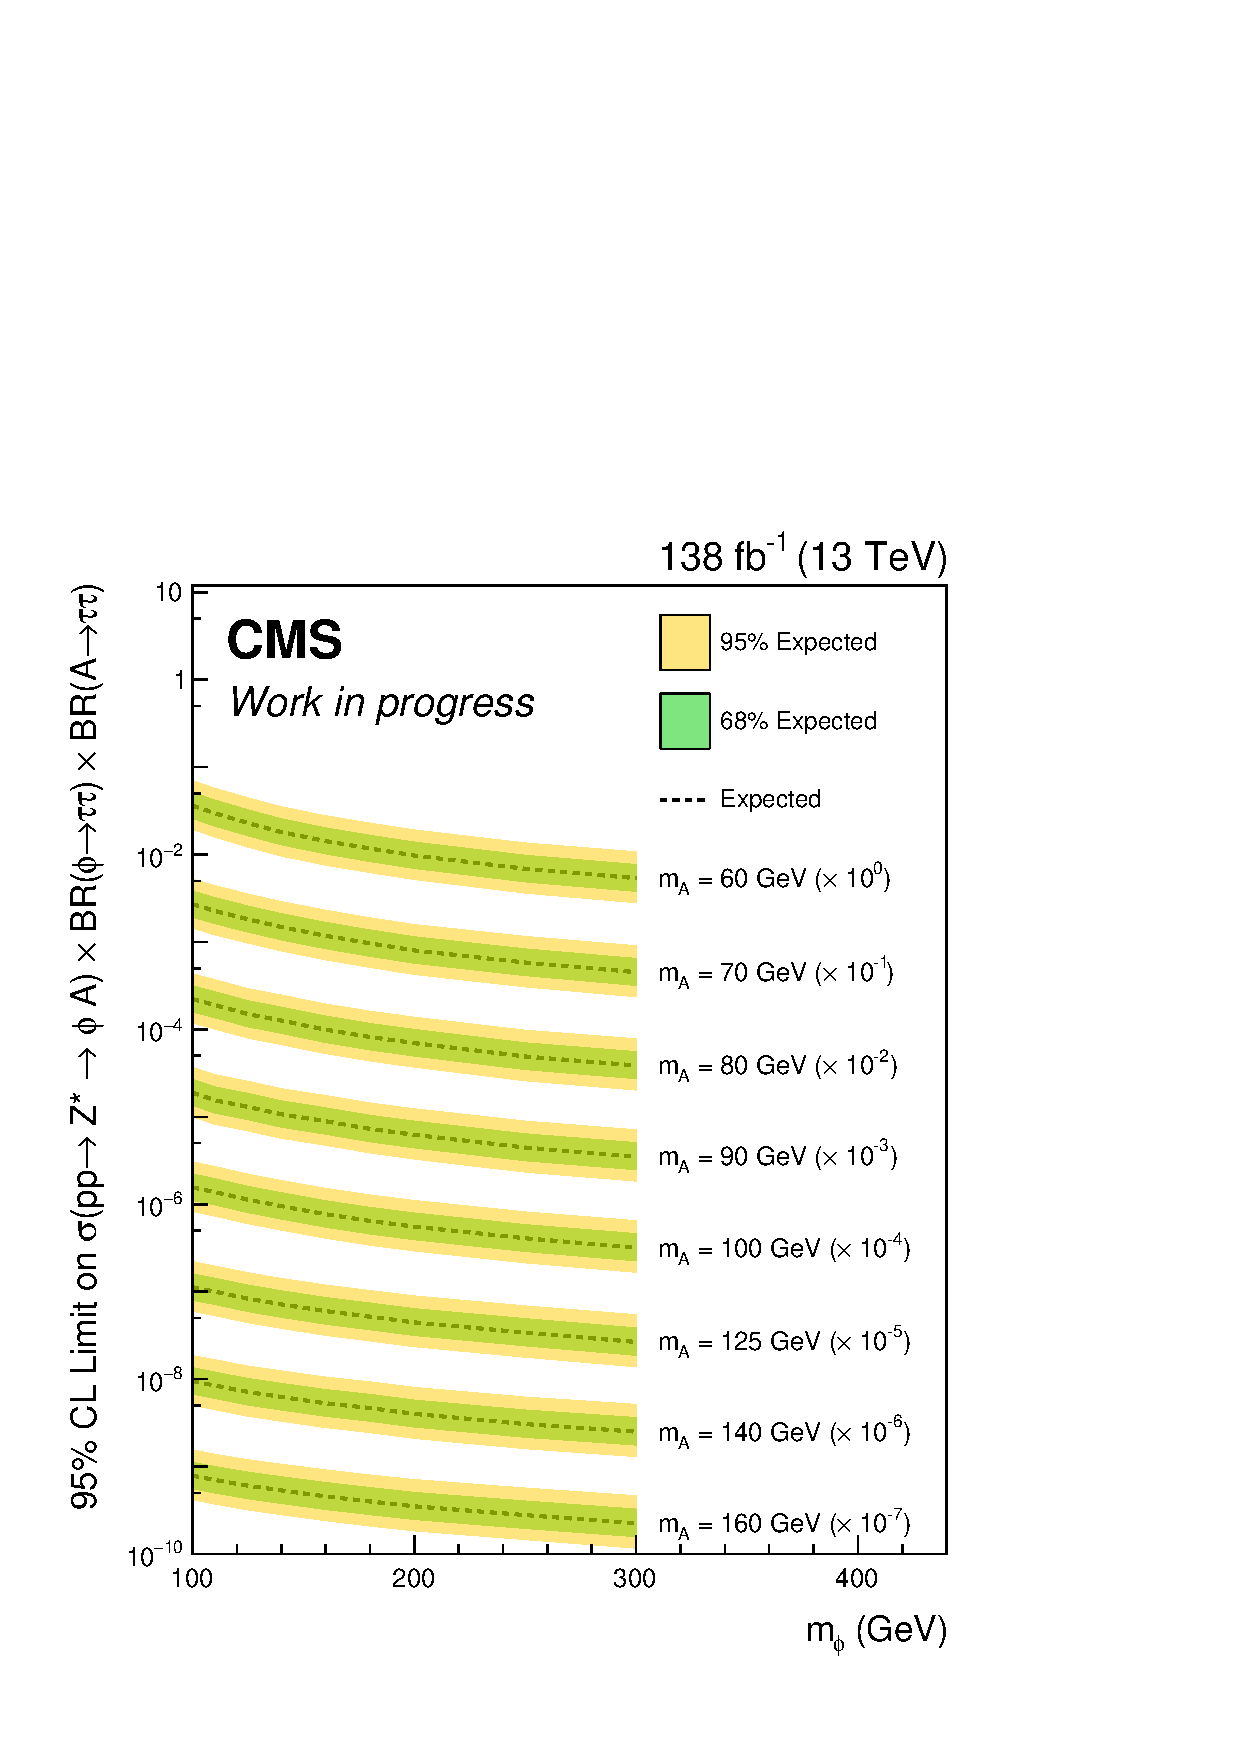
\includegraphics[width=0.8\textwidth]{Figures/model_independent_limit_all.pdf}
\caption[Plot of the model-independent limits on cross-section of the production from an off-shell Z boson multiplied by the branching fractions of $\phi$ and A to $\tau$ pairs.]{Expected (dashed line) and observed (solid line and dots) 95\% CL upper limits on the product of the cross-sections and branching fractions for the decay of both additional Higgs bosons into $\tau$ leptons. Different $m_{A}$ hypotheses are scaled by different orders of magnitudes (written on the plot) to make mass points distinguishable. The dark green and bright yellow bands indicate the central 68\% and 95\% intervals for the expected exclusion limit.}
\label{fig:4tau_mi}
\end{figure}

\subsection{Compatibility}

Similarly to in Section~\ref{sec:sig_and_compat}, the compatibility of the best-fit signal cross-section multiplied by branching fractions in each decay channel is determined, and these are shown in Figure~\ref{fig:4tau_ccc} for a mass hypothesis of $m_{\phi}=m_{A}=100$ GeV for this search.
For this fit the signal strength in each channel is allowed to go negative, although unphysical, to show the data effects in each channel.
The best-fit signal strength of the combined fit is between 1 and 2$\sigma$ below zero.
Four categories fit a signal strength slightly below zero, but the combined fit is mostly dominated by the downward fluctuations of the $e\mu\tauh\tauh$ channel.
The results in each channel are consistent with the zero value within 2$\sigma$.
These conclusions are consistent across any mass hypotheses, again due to the degenerate nature of the signal shapes in the fitted bins.

\section{Model-dependent limits}

The 95\% \ac{CL} exclusion contours, for the type X \ac{2HDM} alignment scenario in the $m_A$-$\tan\beta$ phase space, are shown in Figure~\ref{fig:4tau_md} for two $m_{\phi}$ scenarios of 100 and 200 GeV.
These exclusion limits are \say{top-down} as the cross-sections are unchanged in $\tan\beta$ and the branching fractions to $\tau$ leptons are enhanced as $\tan\beta$ increases.
The cross-section and branching ratios are calculated as described in Section~\ref{sec:4tau_signal_modelling}.
In all cases, as previously observed for the model-independent interpretation, the observed limit lies between the downwards 1 and 2$\sigma$ expected bands. \\


\begin{figure}[!hbtp]
\centering
    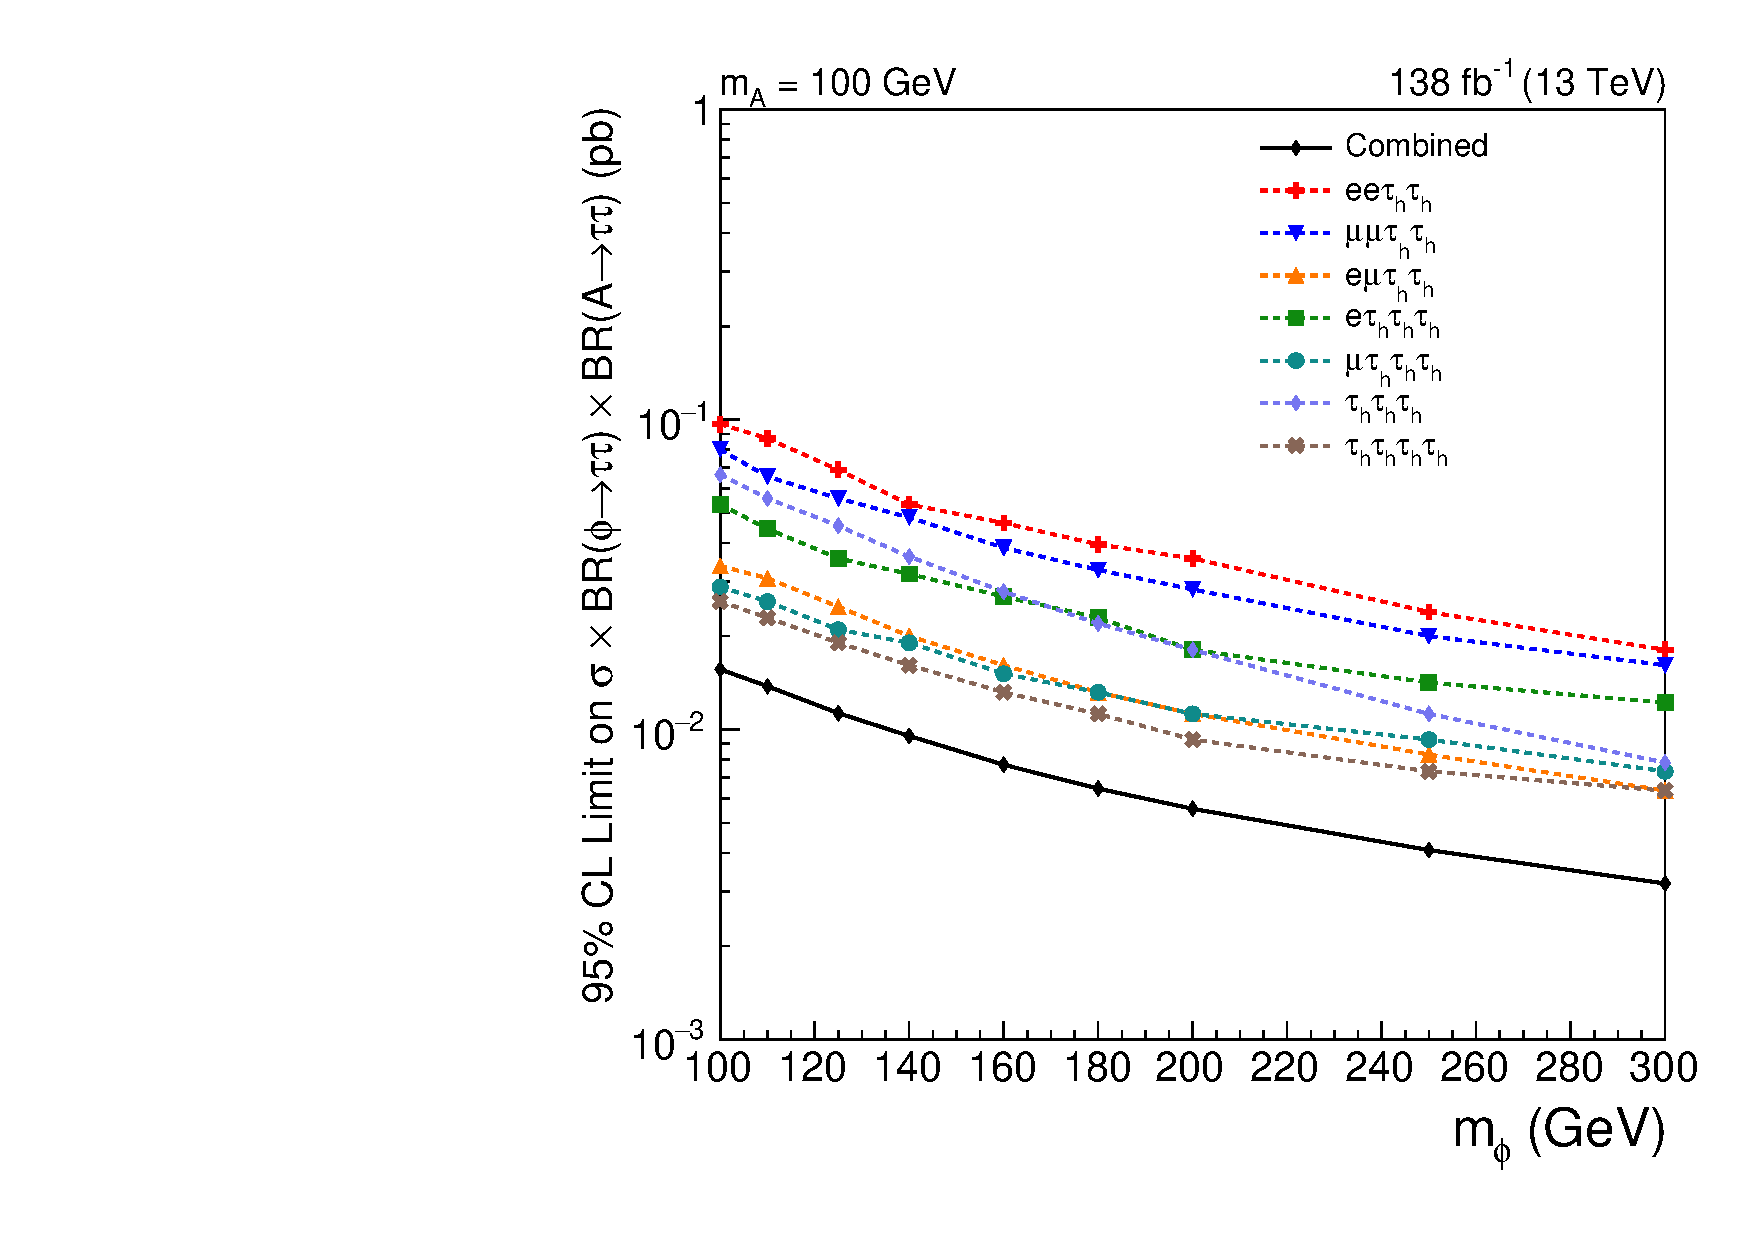
\includegraphics[width=0.6\textwidth]{Figures/limit_comparison_4tau.pdf}
\caption[Plot of the expected model-independent limits split by the $\tau\tau\tau\tau$ decay channels.]{Comparison of the expected 95\% CL upper limits on the product of the cross-sections and branching fractions for the decay into $\tau$ leptons, split by the $\tau\tau\tau\tau$ decay products fit individually.}
\label{fig:4tau_limit_comparison}
\end{figure}

\begin{figure}[!hbtp]
\centering
    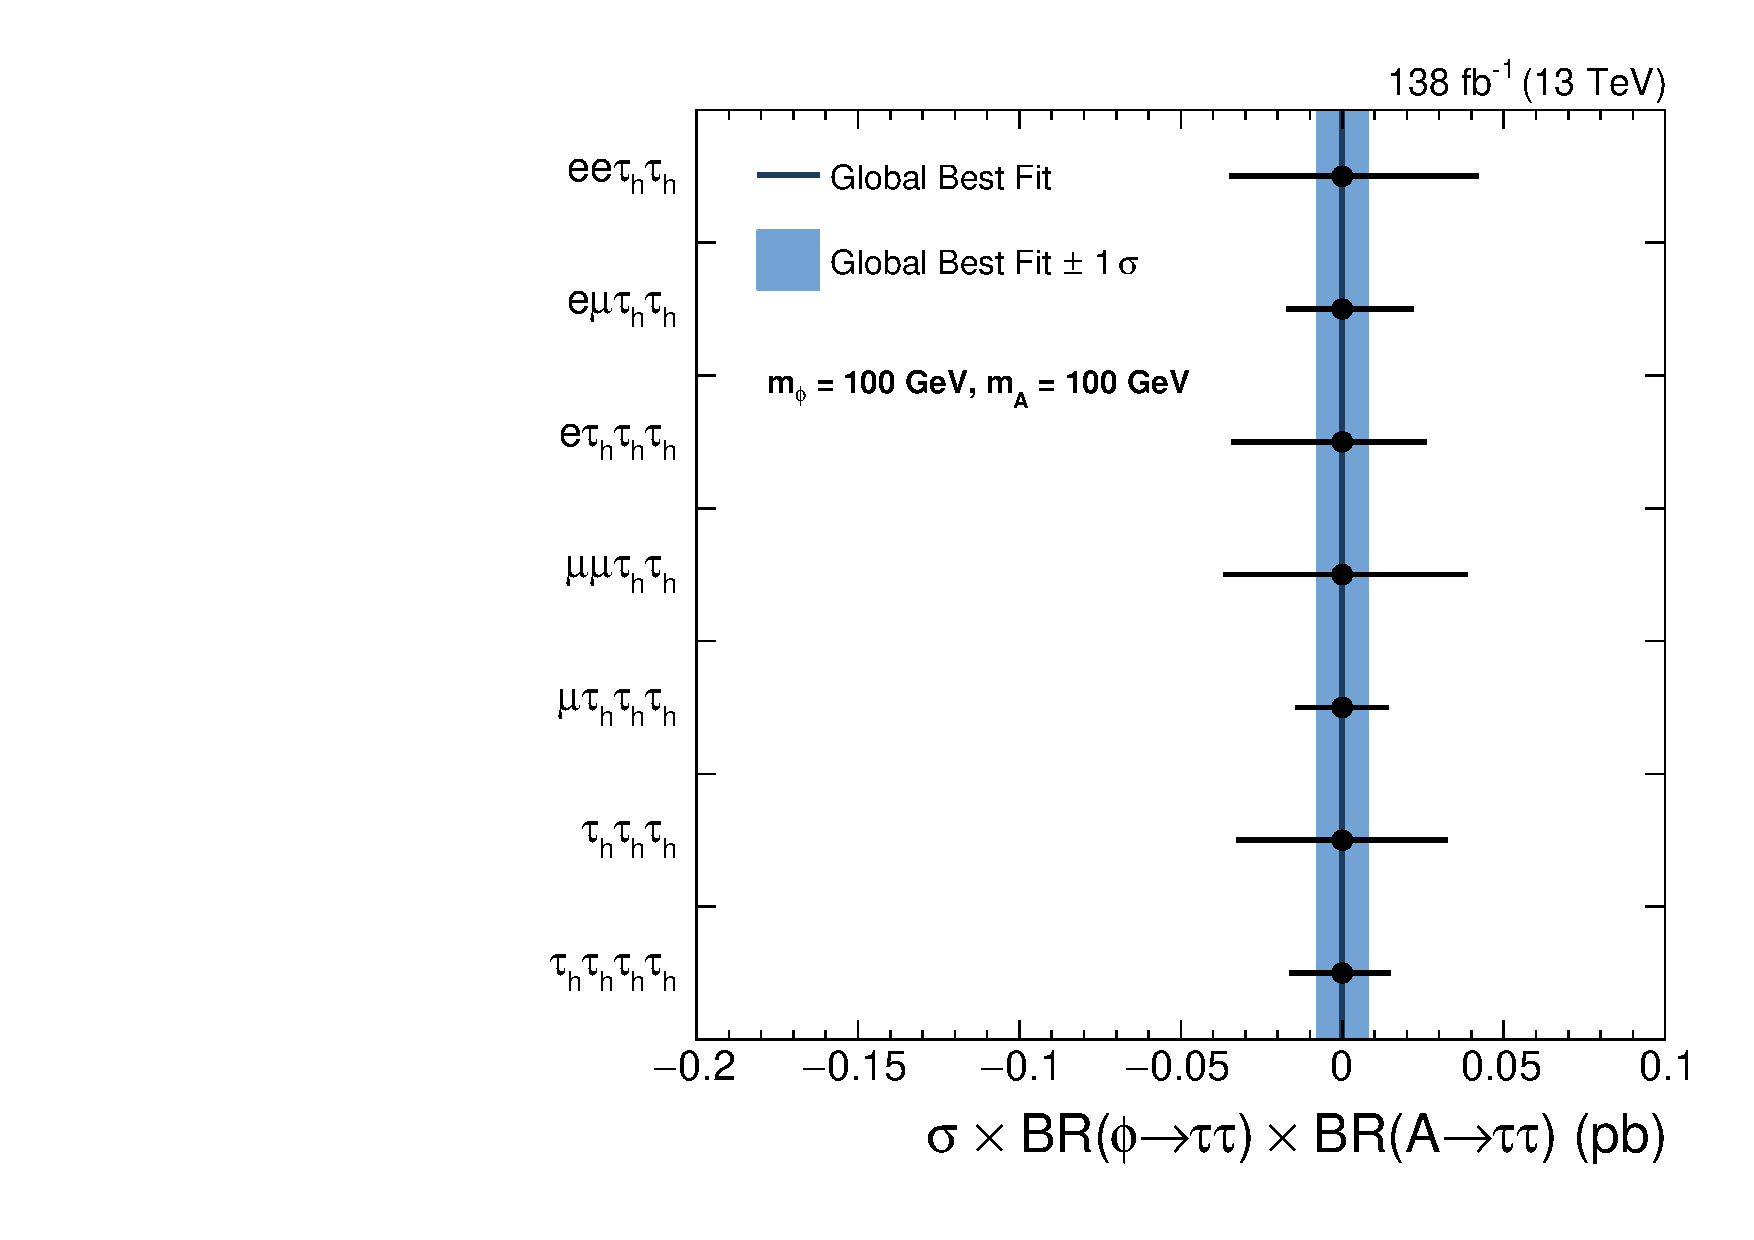
\includegraphics[width=0.6\textwidth]{Figures/ChannelCompatibilityCheck_FitResults_mphi100mA100_channel.pdf}
\caption[Plot of the compatibility of the model-independent results.]{Compatibility plots for the $m_{A}=100$ GeV and $m_{\phi}=100$ GeV mass scenario in analysis decay channels. In each case, the fitted signal strength is decoupled in the bin shown on the plot. The combined best-fit value and its 1$\sigma$ variation are shown by the blue line and band respectively. The black dashed line indicates a signal strength of zero.}
\label{fig:4tau_ccc}
\end{figure}

The $m_{\phi} = 100$ GeV scenario has a moderately flat observed $\tan\beta$ limit between 1.2-1.5, across the $m_{A}$ range.
The very slight weakening of the limit at high values of $m_{A}$ values is because the $A\rightarrow Z\Ph$ decay becomes more kinematically feasible and so the $A\rightarrow\tau\tau$ branching fraction has to compete with this process.
The $\PA\rightarrow Z\Ph$ decay will become dominant if $m_{A}$ is raised much beyond the 160 GeV threshold set in this analysis.
The $m_{\phi} = 200$ GeV scenario's observed limit is weaker at lower values of $m_{A}$, with $\tan\beta$ values ranging from 10 to 1.6 between $m_{A} = 60$ and 125 GeV.
This weakening at lower values of $m_{A}$ happens as the $\PH\rightarrow Z\PA$ decay becomes more kinematically feasible in this region and so competes with $\PH\rightarrow\tau\tau$ for the branching fraction.
This was not present in the $m_{\phi}=100$ GeV scenario as the $\phi$ boson is not heavy enough.
The limit then flattens for the remainder of the $m_{A}$ phase space shown, as the $\PH\rightarrow Z\PA$ and $\PA\rightarrow Zh$ decays only minimally hinder the $\tau\tau$ branching fractions of $\phi$ and $\PA$. \\

Although not shown here, the limits for intermediate $\phi$ masses see similar trends at low $m_{A}$, where the further the $\phi$ and $\PA$ masses are separated the weaker the limit, within this mass range.
At higher values of $m_\phi$ than 200 GeV, it becomes difficult to find stable theories across the $m_{A}$ range. 
This is because if $m_\phi$ and $m_{A}$ are too separated, the values of $\lambda_i$ as shown in Equation~\ref{eqn:lag_2hdm}, can become non-perturbative~\cite{Jueid:2021avn}.
Within the $m_{A}$ allowed regions for this region, the limits follow the same trend as seen at lower values of $m_{\phi}$. \\

\begin{figure}[!hbtp]
\centering
    \subfloat[]{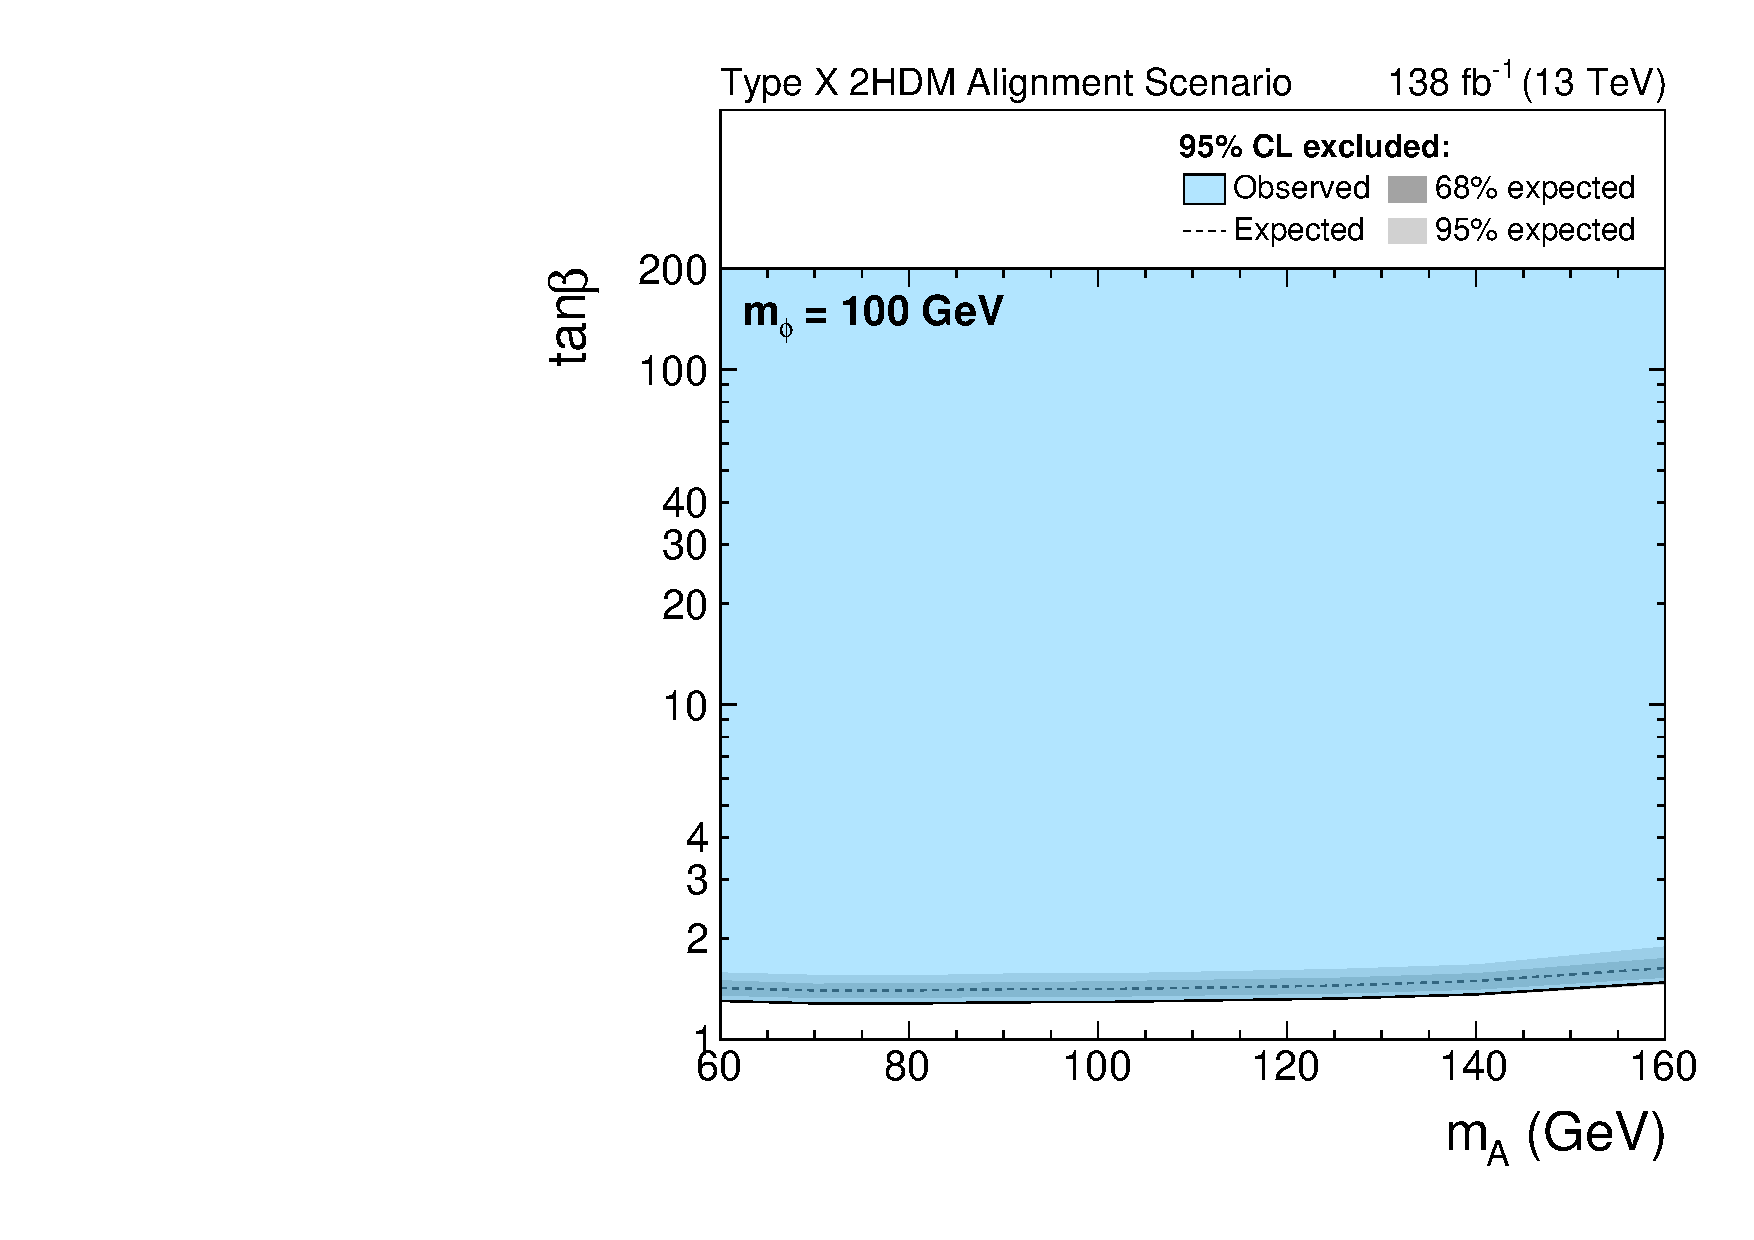
\includegraphics[width=0.65\textwidth]{Figures/md_mphi100.pdf}} \\
    \subfloat[]{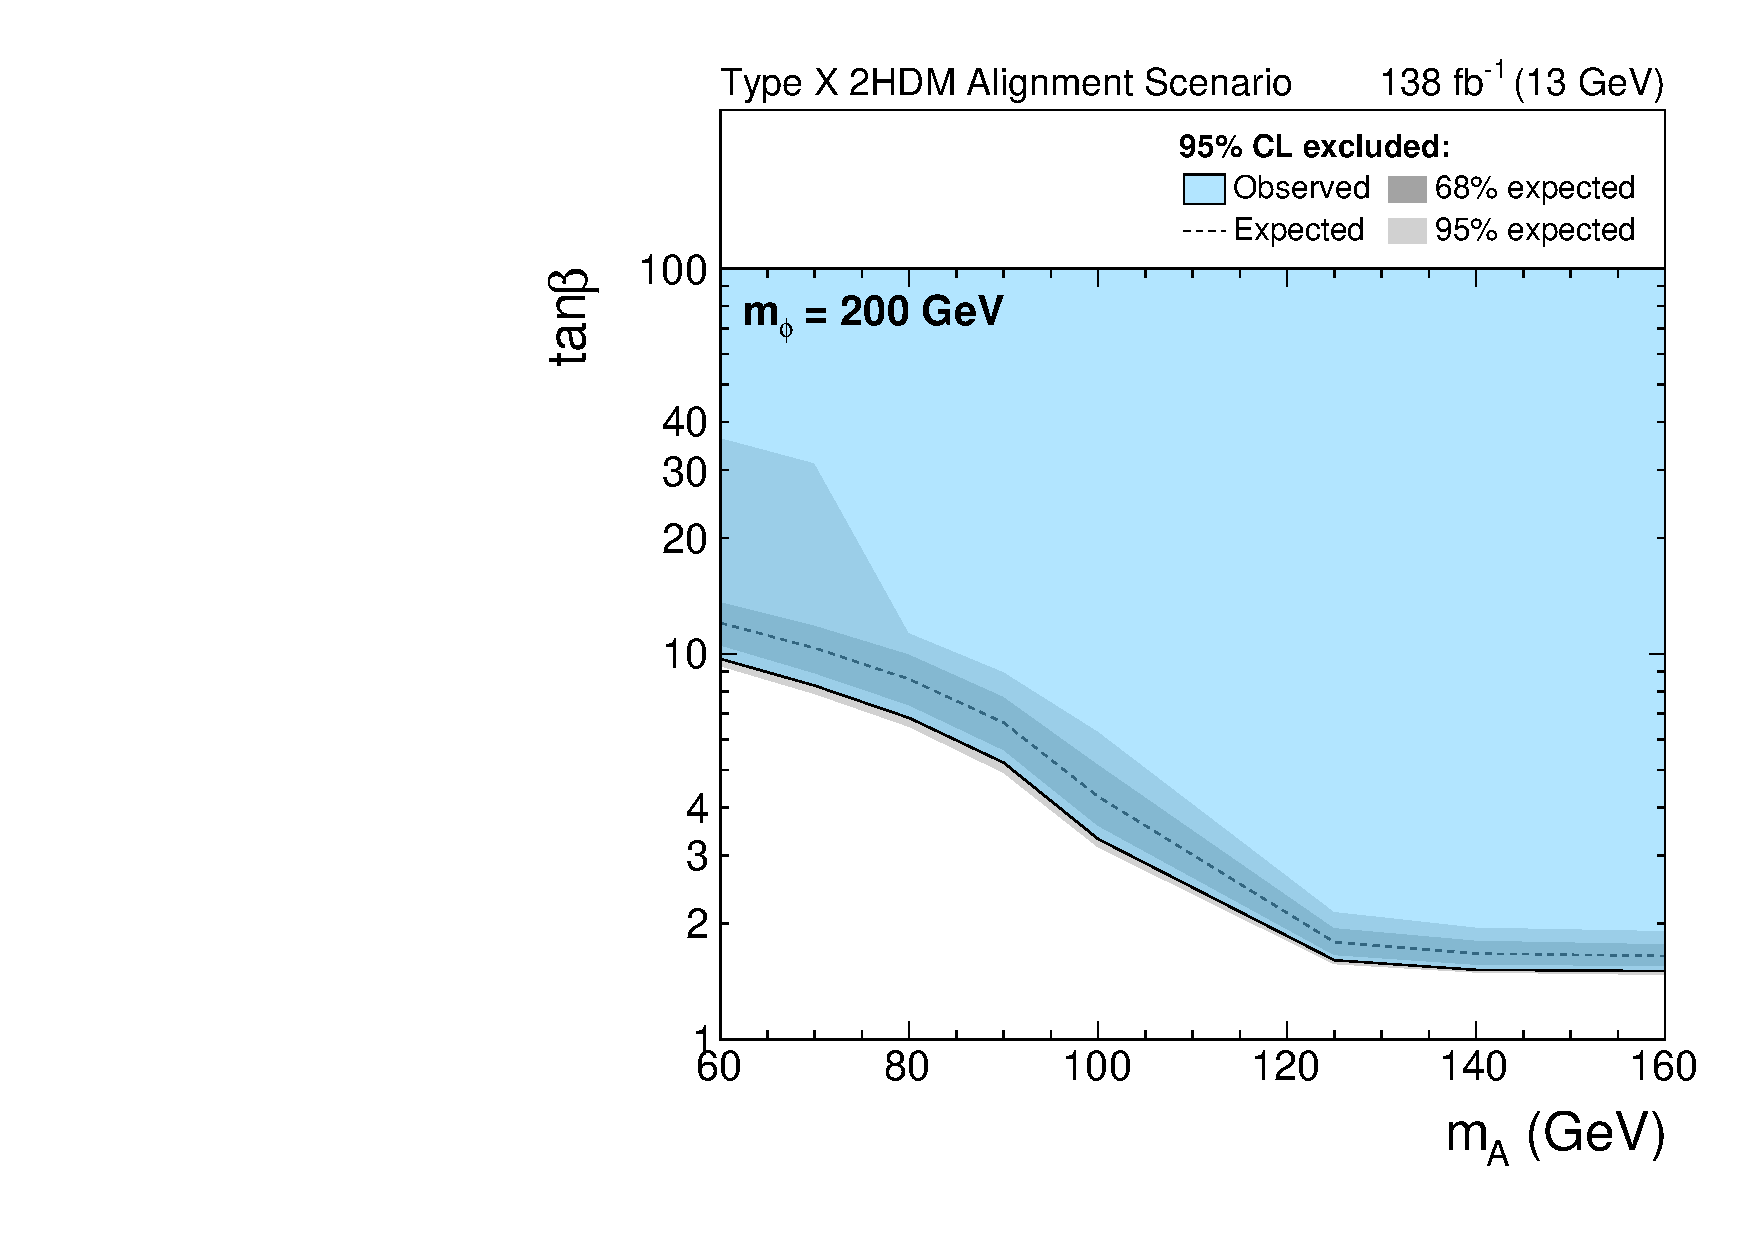
\includegraphics[width=0.65\textwidth]{Figures/md_mphi200.pdf}} 
\caption[Plots of the model-dependent limits in the type X 2HDM alignment scenario.]{Expected and observed 95\% CL exclusion contours on the $m_{A}$-$\tan\beta$ phase space in the type X 2HDM alignment scenario for $m_{\phi}$ scenarios of 100 GeV (a) and 200 GeV (b). The exclusion limit only on background expectation is shown as a dashed black line, the dark and bright grey bands show the 68\% and 95\% intervals of the expected exclusion and the observed exclusion contour is shown by the blue area.}
\label{fig:4tau_md}
\end{figure}

95\% \ac{CL} limits are also set outside of the alignment scenario.
This is done by varying relevant alignment parameter, $\cos(\beta-\alpha)$ or $\sin(\beta-\alpha)$ depending on $m_\phi$, with respect to $\tan\beta$ for the individual mass hypothesis.
Two of these are shown in Figure~\ref{fig:4tau_cosbma} for the mass scenario of $m_{\phi} = 200$ GeV and $m_{A} = 100$ GeV, as well as $m_{\phi} = 200$ GeV and $m_{A} = 160$.
The observed limit lies in the equivalent place compared to the expected as seen in all limit setting for this analysis.
The alignment limit at these mass points is equivalent to the limit set at $\cos(\beta-\alpha) = 0$.
The shapes of the limits represent the region where the loss of cross-section and branching ratio for $\phi$, out of the alignment scenario and at lower $\tan\beta$, is too large that the theory cannot be excluded.
The shapes are symmetric in $\cos(\beta-\alpha)$ as no sign dependence is measurable from this process.
The widening and narrowing of the limit band in $\tan\beta$ is due to the shape of the branching fractions of $\phi$, as shown in Figure~\ref{fig:4tau_br_2d}.
The widest constraint from this search on $|\cos(\beta-\alpha)|$ is at approximately 0.5 at a $\tan\beta$ around 20.

\begin{figure}[!hbtp]
\centering
    \subfloat[]{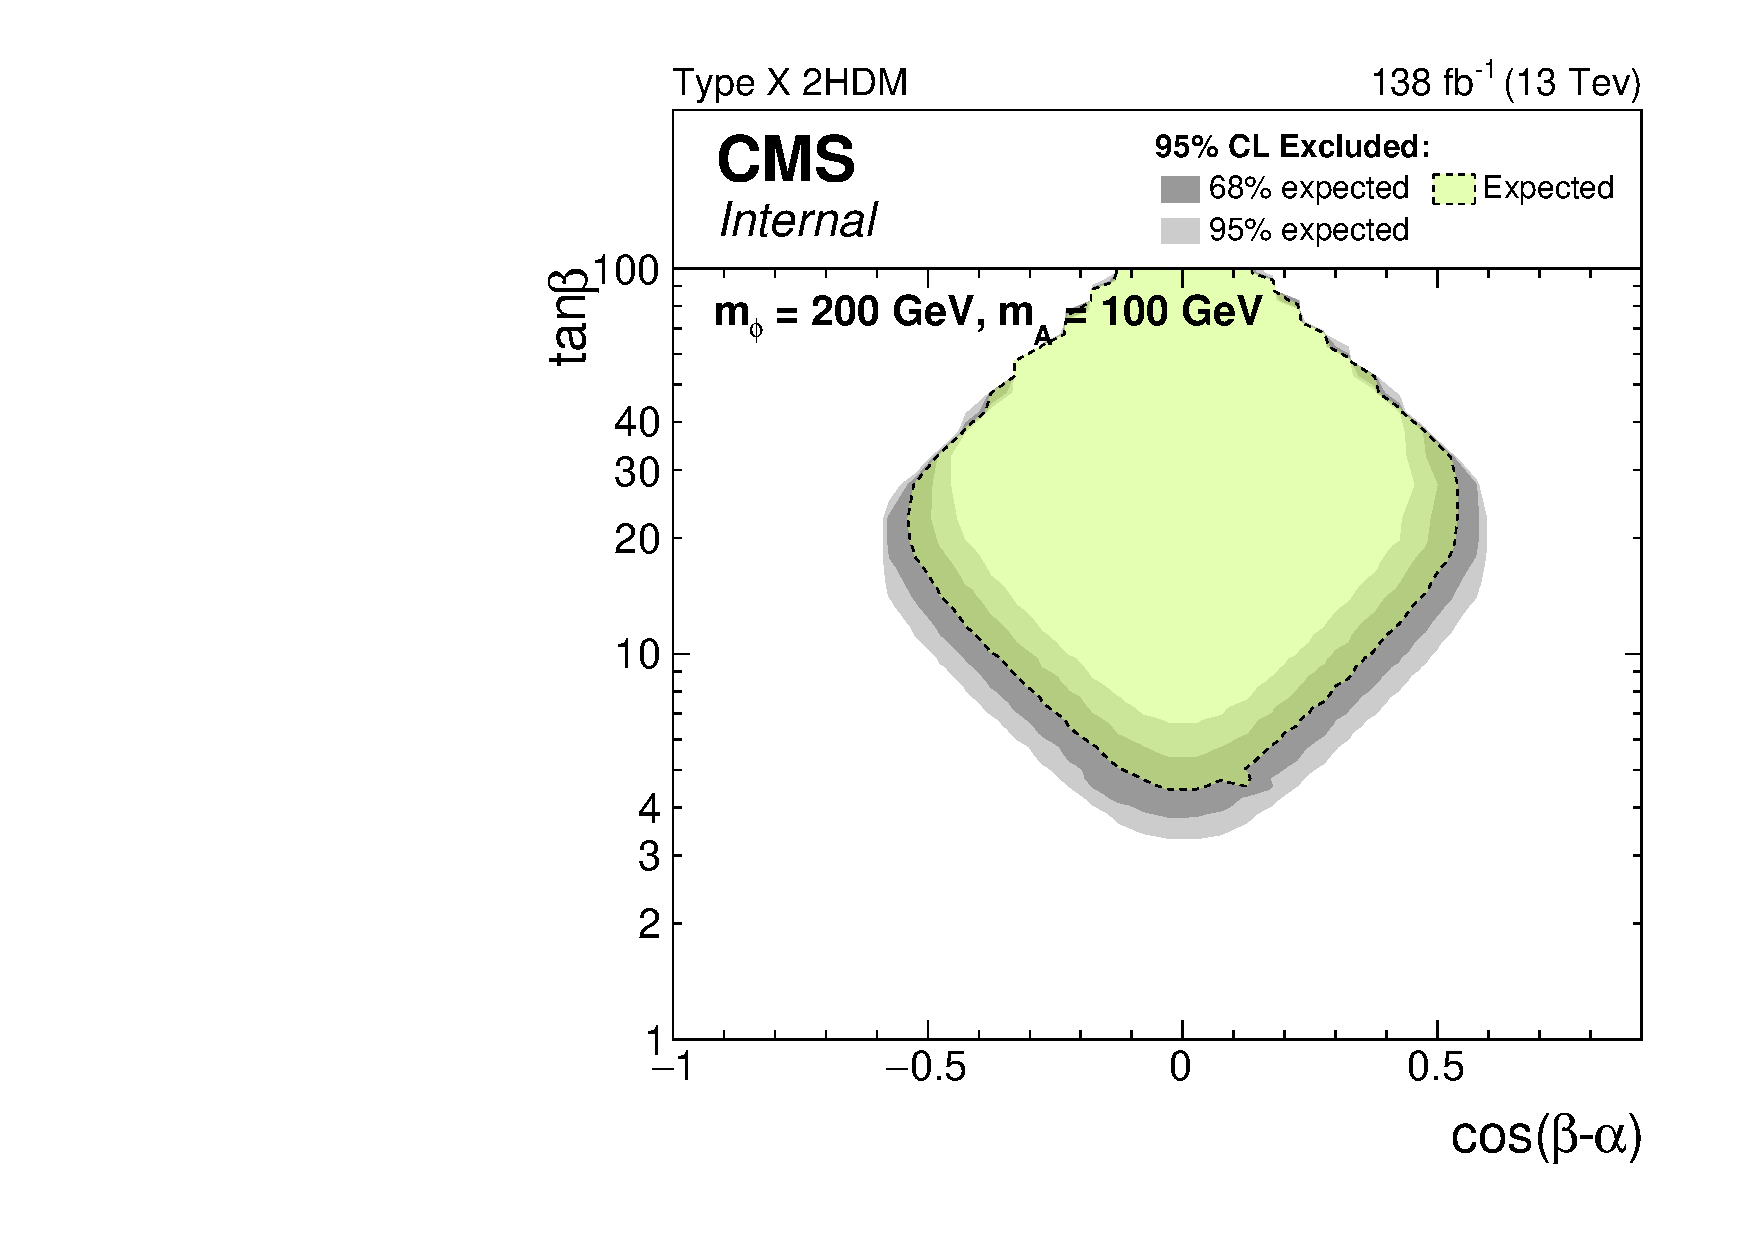
\includegraphics[width=0.65\textwidth]{Figures/csbma_phi200A100.pdf}} \\
    \subfloat[]{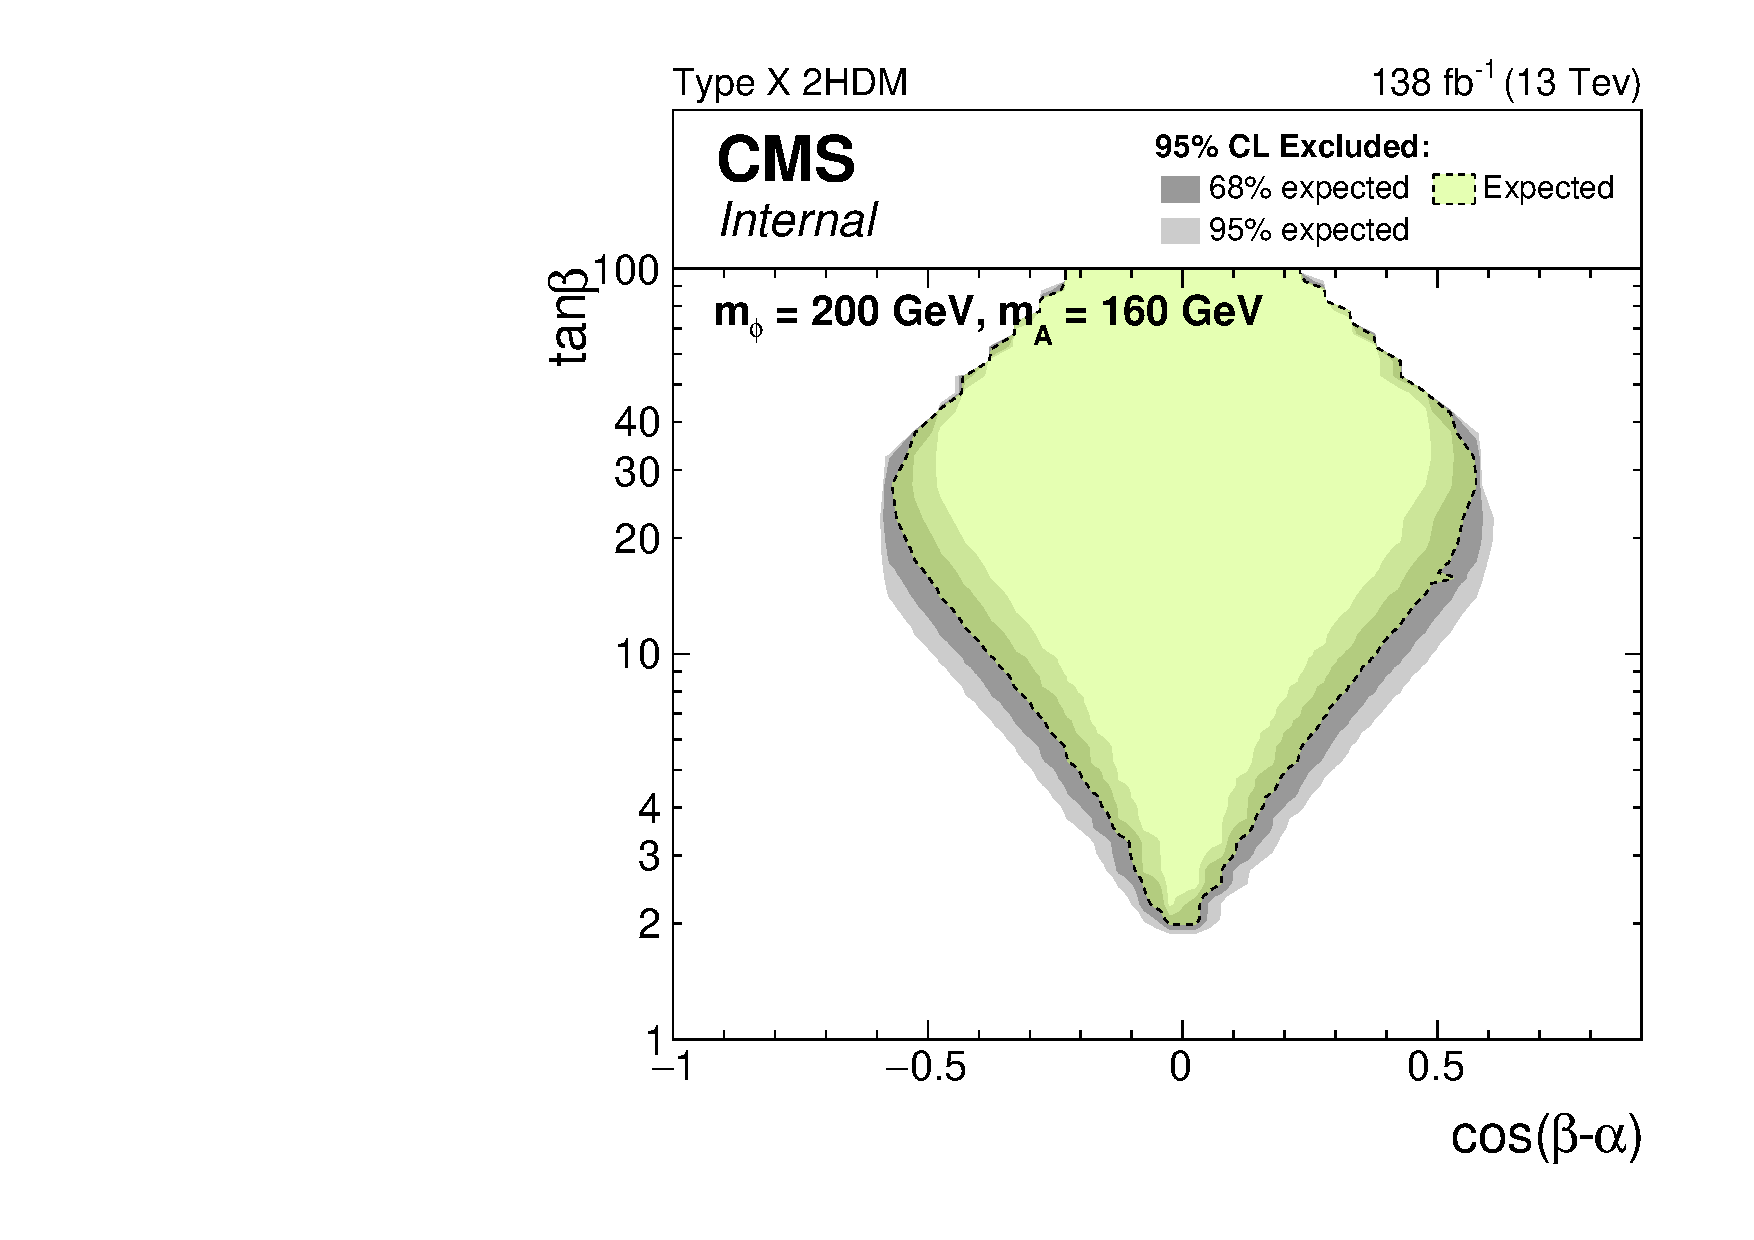
\includegraphics[width=0.65\textwidth]{Figures/csbma_phi200A160.pdf}} 
\caption[Plots of the model-dependent limits in the type X 2HDM, out of the alignment scenario.]{Expected and observed 95\% CL exclusion contours on the $\cos(\beta-\alpha)$-$\tan\beta$ phase space in the type X 2HDM alignment scenario with $m_{\phi}$ equal to 200 GeV and $m_{A}$ scenarios of 100 GeV (a) and 160 GeV (b). The exclusion limit only on background expectation is shown as a dashed black line, the dark and bright grey bands show the 68\% and 95\% intervals of the expected exclusion and the observed exclusion contour is shown by the blue area.}
\label{fig:4tau_cosbma}
\end{figure}
